% -*- Mode:TeX -*-

%% IMPORTANT: The official thesis specifications are available at:
%%            http://libraries.mit.edu/archives/thesis-specs/
%%
%%            Please verify your thesis' formatting and copyright
%%            assignment before submission. If you notice any
%%            discrepancies between these templates and the 
%%            MIT Libraries' specs, please let us know
%%            by e-mailing thesis@mit.edu

%% The documentclass options along with the pagestyle can be used to generate
%% a technical report, a draft copy, or a regular thesis. You may need to
%% re-specify the pagestyle after you \include cover.tex. For more
%% information, see the first few lines of mitthesis.cls. 

%\documentclass[12pt,vi,twoside]{mitthesis}
%%
%%  If you want your thesis copyright to you instead of MIT, use the
%%  ``vi'' option, as above.
%%
%\documentclass[12pt,twoside,leftblank]{mitthesis}
%%
%% If you want blank pages before new chapters to be labelled ``This
%% Page Intentionally Left Blank'', use the ``leftblank'' option, as
%% above. 

%aps,prd,longbibliography]%{revtex4-1}
%CHANGE IT TO TWO SIDE!!!! FOR FORMAL PRINTING$
%\documentclass[12pt,twoside,vi]{mitthesis}
\documentclass[12pt,oneside,vi]{mitthesis}

\usepackage{lgrind}
\usepackage{tabularx}
%% These have been added at the request of the MIT Libraries, because
%% some PDF conversions mess up the ligatures.  -LB, 1/22/2014
\usepackage{cmap}
\usepackage{float}
\usepackage{xcolor}
\usepackage{wrapfig}
\usepackage{graphicx}
\usepackage{geometry}
\usepackage{longtable}

\usepackage[page,toc,titletoc,title]{appendix}

\usepackage{amsmath} % for \boxed and \smash[b] macros
\usepackage{booktabs}% for \midrule and \cmidrule macro
\usepackage{braket}
\usepackage[compat=1.1.0]{tikz-feynman}
\usepackage{siunitx}  % Used for formatting numbers

\usepackage{lmodern}
\usepackage{xpatch}
\usepackage{xcolor}
\usepackage{graphicx}
\usepackage{geometry}
\usepackage{listings}
%\usepackage{tocbibind}
\usepackage{xpatch}
\usepackage{slashed}
\usepackage{adjustbox}
\usepackage{xcolor}
\usepackage{textcomp}
%\usepackage{gensymb} %causes issues with degree command
\usepackage{tocloft}
\usepackage{float}
%\usepackage{notoccite}
%\usepackage[style=authoryear]{biblatex}
\usepackage[backend=biber, citestyle=authoryear, bibstyle=numeric, sortcites, sorting=nty, backref, natbib, hyperref]{biblatex}
%\usepackage[style=phys]{biblatex}
%use below if not biblatex
%\bibliographystyle{apsrev}
%\bibliographystyle{unsrtnat}
%\usepackage[square,numbers]{natbib}
\addbibresource{Chapters/Postamble/bib/references.bib}

\usepackage{caption}
\usepackage{multirow}
\usepackage{subfig}
%\captionsetup[subfloat]{position=top,
%  farskip=10pt,topadjust=0pt,captionskip=10pt,
%  nearskip=10pt,margin=10pt}


\DeclareCiteCommand{\cite}
  {\usebibmacro{prenote}}
  {\usebibmacro{citeindex}%
   \printtext[bibhyperref]{\usebibmacro{cite}}}
  {\multicitedelim}
  {\usebibmacro{postnote}}

\DeclareCiteCommand*{\cite}
  {\usebibmacro{prenote}}
  {\usebibmacro{citeindex}%
   \printtext[bibhyperref]{\usebibmacro{citeyear}}}
  {\multicitedelim}
  {\usebibmacro{postnote}}

\DeclareCiteCommand{\parencite}[\mkbibparens]
  {\usebibmacro{prenote}}
  {\usebibmacro{citeindex}%
    \printtext[bibhyperref]{\usebibmacro{cite}}}
  {\multicitedelim}
  {\usebibmacro{postnote}}

\DeclareCiteCommand*{\parencite}[\mkbibparens]
  {\usebibmacro{prenote}}
  {\usebibmacro{citeindex}%
    \printtext[bibhyperref]{\usebibmacro{citeyear}}}
  {\multicitedelim}
  {\usebibmacro{postnote}}

\DeclareCiteCommand{\footcite}[\mkbibfootnote]
  {\usebibmacro{prenote}}
  {\usebibmacro{citeindex}%
  \printtext[bibhyperref]{ \usebibmacro{cite}}}
  {\multicitedelim}
  {\usebibmacro{postnote}}

\DeclareCiteCommand{\footcitetext}[\mkbibfootnotetext]
  {\usebibmacro{prenote}}
  {\usebibmacro{citeindex}%
   \printtext[bibhyperref]{\usebibmacro{cite}}}
  {\multicitedelim}
  {\usebibmacro{postnote}}

\DeclareCiteCommand{\textcite}
  {\boolfalse{cbx:parens}}
  {\usebibmacro{citeindex}%
   \printtext[bibhyperref]{\usebibmacro{textcite}}}
  {\ifbool{cbx:parens}
     {\bibcloseparen\global\boolfalse{cbx:parens}}
     {}%
   \multicitedelim}
  {\usebibmacro{textcite:postnote}}







%include if want to check unused referneces and uncomment nocite{*}
%\usepackage{refcheck}


\usepackage{tikz}
\usetikzlibrary{arrows,shapes.geometric,positioning,fit,backgrounds,calc, arrows.meta,chains,shapes.arrows}

\makeatletter
\tikzset{west above/.code=\tikz@lib@place@handle@{#1}{south west}{0}{1}{north west}{1}}
\tikzset{west below/.code=\tikz@lib@place@handle@{#1}{north west}{0}{-1}{south west}{1}}
\tikzset{east above/.code=\tikz@lib@place@handle@{#1}{south east}{0}{1}{north east}{1}}
\tikzset{east below/.code=\tikz@lib@place@handle@{#1}{north east}{0}{-1}{south east}{1}}
\makeatother

\newcommand\headercell[1]{%
   \smash[b]{\begin{tabular}[t]{@{}c@{}} #1 \end{tabular}}}
\usepackage[colorlinks = true,
            linkcolor = blue,
            urlcolor  = blue,
            citecolor = blue,
            anchorcolor = blue]{hyperref}

\newcommand{\Lumi}{\ensuremath{\textcolor{gray}{ \mathcal{L}}}}
\newcommand{\Lumispace}{\ensuremath{\textcolor{gray}{ \mathcal{L} }}}

\newcommand{\Lumiint}{\ensuremath{\textcolor{gray}{ \mathcal{L}_{int}}} }

\newcommand{\counts}{\ensuremath{\textcolor{red}{N_{exp}}}}



\newcommand{\Nexp}{$N_{\text{exp}}$}
\newcommand{\Ntruth}{$N_{\text{truth}}$}
\newcommand{\Nsim}{$N_{\text{sim}}$}
\newcommand{\Ngen}{$N_{\text{gen}}$}

\newcommand{\xsec}{cross section }
\newcommand{\xsecs}{cross sections }
\newcommand{\Xsec}{Cross section }
\newcommand{\Xsecs}{Cross sections }
\newcommand{\xsecp}{cross section. }
\newcommand{\xsecsp}{cross sections. }
\newcommand{\Xsecp}{Cross section. }
\newcommand{\Xsecsp}{Cross sections. }
\newcommand{\dvpip}{DV$\pi^0$P }

\newcommand{\figref}[1]{Fig.~\ref{#1}}
\newcommand{\tabref}[1]{Table~\ref{#1}}
\newcommand{\chref}[1]{(Ch.~\ref{#1})}
\newcommand{\secref}[1]{(sec.~\ref{#1})}
\newcommand{\Secref}[1]{(Sec.~\ref{#1})}

\newcommand{\appref}[1]{(app.~\ref{#1})}
\newcommand{\Appref}[1]{(App.~\ref{#1})}




%For scaled data reduction drawing:
%normal cube
\newcommand{\Depth}{10}
\newcommand{\Height}{10}
\newcommand{\Width}{10}

% smaller cube
\newcommand{\smallDepth}{1.25}
\newcommand{\smallHeight}{1.25}
\newcommand{\smallWidth}{1.25}

% even smaller cube
\newcommand{\evenSmallerDepth}{0.134}
\newcommand{\evenSmallerHeight}{0.134}
\newcommand{\evenSmallerWidth}{0.134}

% larger cube
\newcommand{\largerDepth}{2.94}
\newcommand{\largerHeight}{2.94}
\newcommand{\largerWidth}{2.94}

% even smaller cube
\newcommand{\tinyDepth}{0.08}
\newcommand{\tinyHeight}{0.08}
\newcommand{\tinyWidth}{0.08}


\usepackage{adjustbox}


%labelandremeber from https://tex.stackexchange.com/questions/459508/how-can-i-repeat-a-formula-without-copying-it
\newcommand\labelAndRemember[2]
  {\expandafter\gdef\csname labeled:#1\endcsname{#2}%
   \label{#1}#2}
\newcommand\recallLabel[1]
   {\csname labeled:#1\endcsname\tag{\ref{#1}}}

%\usepackage[square,numbers,sort&compress]{natbib}

\setcounter{tocdepth}{2}
\setcounter{secnumdepth}{5}

%\bibliographystyle{ieeetr}
%\usepackage{natbib}
%\setcitestyle{numbers}
%\usepackage{apacite}
%\bibliographystyle{apacite}

\usepackage[T1]{fontenc}
\pagestyle{plain}


\definecolor{britishracinggreen}{rgb}{0.0, 0.26, 0.15}
\definecolor{burgundy}{rgb}{0.5, 0.0, 0.13}


% Chiral Even GPDs
\newcommand{\GPDH}{\textcolor{lightred}{${H}$}}
\newcommand{\GPDHEQ}{\textcolor{lightred}{{H}}}
\newcommand{\GPDE}{\textcolor{lightgreen}{${E}$}}
\newcommand{\GPDEEQ}{\textcolor{lightgreen}{{E}}}
\newcommand{\GPDHtilde}{\textcolor{lightorange}{$\tilde{H}$}}
\newcommand{\GPDHtildeEQ}{\textcolor{lightorange}{\tilde{H}}}
\newcommand{\GPDEtilde}{\textcolor{lightblue}{$\tilde{E}$}}
\newcommand{\GPDEtildeEQ}{\textcolor{lightblue}{\tilde{E}}}

%Chiral Odd GPDs
\newcommand{\GPDHT}{\textcolor{darkred}{$H_T$}}
\newcommand{\GPDHTEQ}{\textcolor{darkred}{H_T}}
\newcommand{\GPDET}{\textcolor{darkgreen}{$E_T$}}
\newcommand{\GPDETEQ}{\textcolor{darkgreen}{E_T}}
\newcommand{\GPDHTtilde}{\textcolor{darkorange}{$\tilde{H}_T$}}
\newcommand{\GPDHTtildeEQ}{\textcolor{darkorange}{\tilde{H}_T}}
\newcommand{\GPDETtilde}{\textcolor{darkblue}{$\tilde{E}_T$}}
\newcommand{\GPDETtildeEQ}{\textcolor{darkblue}{\tilde{E}_T}}
\newcommand{\GPDETbar}{\textcolor{mypurp}{$\bar{E}_T$}}
\newcommand{\GPDETbarEQ}{\textcolor{mypurp}{\bar{E}_T}}
\usepackage{fancyhdr}



%%%%%% COMMENT THIS SECTION OUT IF YOU DON'T WANT TOC LINK IN EACH PAGE
\fancyhead{} % clear all header fields
\renewcommand{\headrulewidth}{0pt} % no line in header area
\fancyfoot{} % clear all footer fields
%\fancyfoot[LE,RO]{\thepage}           % page number in "outer" position of footer line
%\fancyfoot[C]{\thepage \quad \quad \hyperlink{page.5}{TOC} \quad \quad Flow: \ref{fig:ProcessFlowchart}}
% With TOC
\fancyfoot[C]{\thepage \quad \quad \hyperlink{page.5}{ToC}}
%plain:
%\fancyfoot[C]{\thepage}

%\fancyhf{}
%\fancyhead[RO]{\textsc{\nouppercase{\newlinetospace{{\leftmark}}\quad\thepage}}}

\newcommand{\listequationsname}{List of Equations}
\newcommand{\myequations}[1]{\addcontentsline{equ}{myequations}{\protect\numberline{\theequation}\quad \quad #1}\par}

\newcommand{\listtodo}{List of To Do Items}
\newcommand{\mytodo}[1]{\addcontentsline{todo}{mytodo}{\protect\numberline{\theequation}\quad \quad #1}\par}

\newcommand{\todo}[1]{\iflong \textcolor{red}{#1} \mytodo{#1} \else \fi}

\newcommand{\sci}[1]{$\times 10^{#1}$}

\newcommand{\Moller}{ M\"oller }



\usepackage{siunitx}


%% This bit allows you to either specify only the files which you wish to
%% process, or `all' to process all files which you \include.
%% Krishna Sethuraman (1990).

%\typein [\files]{Enter file names to process, (chap1,chap2 ...), or `all' to process all files:}
%\def\all{all}
%\ifx\files\all \typeout{Including all files.} \else %\typeout{Including only \files.} \includeonly{\files} \fi

\definecolor{mygreen}{RGB}{14, 176, 9}
\definecolor{correctionfactors}{RGB}{11, 122, 25}

\definecolor{myyellow}{RGB}{204, 204, 10}
\definecolor{mypink}{RGB}{255, 51, 255}
\definecolor{mypurp}{RGB}{153, 21, 255}
\definecolor{lightred}{RGB}{255, 132, 145}
\definecolor{darkred}{RGB}{225, 0, 0}
\definecolor{lightorange}{RGB}{255, 200, 84}
\definecolor{darkorange}{RGB}{225, 150, 0}
\definecolor{lightgreen}{RGB}{85, 255, 91}
\definecolor{darkgreen}{RGB}{0, 170, 6}
\definecolor{lightblue}{RGB}{88, 200, 255}
\definecolor{darkblue}{RGB}{0, 81, 203}
\definecolor{sigmaT}{RGB}{0, 0, 0}
\definecolor{sigmaL}{RGB}{0, 0, 0}
\definecolor{sigmaLT}{RGB}{252, 3, 3}
\definecolor{sigmaTT}{RGB}{3, 32, 252}


%This is to have multiple URLs in the bibliography be cited correctly
%This must be placed after any packages like url or hyperrref
%Code from https://tex.stackexchange.com/questions/57865/how-to-use-multiple-urls-for-one-bibtex-reference
\renewbibmacro*{url}{\printfield[url]{urlraw}}

\let\URL\url
\makeatletter
\def\url{\begingroup \catcode`\%=12\catcode`\#=12\relax\printurl}
\def\printurl#1{\@URL#1 \@nil\endgroup}
\def\@URL#1 #2\@nil{\URL{#1}\ifx\relax#2\relax \else; \url{#2\relax}\fi}
\makeatother

\begin{document}

\newif\iflong

%Turn todo section on /off
%on:
%\longtrue
%off: 
\longfalse
 
%  \iflong \lipsum[1] \else short version \fi


%%%%%%%%%%%%%%%%%%%%%%%%%%%%%%%%%%%%%%%%%%%%%%%%%%%% PREAMBLE %%%%%%%%%%%%%%%%%%%%%%%%%%%%%%%%%%%%%%%%%%%%%%%%%%%%%%%%%%%

% NOTE:
% These templates make an effort to conform to the MIT Thesis specifications,
% however the specifications can change. We recommend that you verify the
% layout of your title page with your thesis advisor and/or the MIT 
% Libraries before printing your final copy.

\title{Measurement of the Deeply Virtual Neutral Pion Electroproduction Cross Section at the Thomas Jefferson National Accelerator Facility at 10.6 GeV}
%bragtitle
%\title{Constraining Generalized Parton Distributions for Proton Tomography Through Measurement of the Deeply Virtual Neutral Pion Electroproduction Cross Section at the Thomas Jefferson National Accelerator Facility at 10.6 GeV with Unbinned Iterative Bayesian Unfolding}

\author{Robert Johnston}
% If you wish to list your previous degrees on the cover page, use the 
% previous degrees command:
%       \prevdegrees{A.A., Harvard University (1985)}
% You can use the \\ command to list multiple previous degrees
%       \prevdegrees{B.S., University of California (1978) \\
%                    S.M., Massachusetts Institute of Technology (1981)}
\department{Department of Physics}

% If the thesis is for two degrees simultaneously, list them both
% separated by \and like this:
% \degree{Doctor of Philosophy \and Master of Science}
\degree{Interdisciplinary PhD in Physics and Statistics}

% As of the 2007-08 academic year, valid degree months are September, 
% February, or June.  The default is June.
\degreemonth{August}
\degreeyear{2023}
%\degreemonth{\textcolor{red}{CONFIDENTIAL}}
%\degreeyear{\textcolor{red}{DRAFT}}
\thesisdate{August, 2023}

%% By default, the thesis will be copyrighted to MIT.  If you need to copyright
%% the thesis to yourself, just specify the `vi' documentclass option.  If for
%% some reason you want to exactly specify the copyright notice text, you can
%% use the \copyrightnoticetext command.  
%\copyrightnoticetext{\copyright IBM, 1990.  Do not open till Xmas.}

% If there is more than one supervisor, use the \supervisor command
% once for each.
\supervisor{Richard Milner}{Professor of Physics}

% This is the department committee chairman, not the thesis committee
% chairman.  You should replace this with your Department's Committee
% Chairman.
\chairman{Lindley Winslow}{Associate Department Head of Physics}

% Make the titlepage based on the above information.  If you need
% something special and can't use the standard form, you can specify
% the exact text of the titlepage yourself.  Put it in a titlepage
% environment and leave blank lines where you want vertical space.
% The spaces will be adjusted to fill the entire page.  The dotted
% lines for the signatures are made with the \signature command.
\maketitle

% The abstractpage environment sets up everything on the page except
% the text itself.  The title and other header material are put at the
% top of the page, and the supervisors are listed at the bottom.  A
% new page is begun both before and after.  Of course, an abstract may
% be more than one page itself.  If you need more control over the
% format of the page, you can use the abstract environment, which puts
% the word "Abstract" at the beginning and single spaces its text.

%% You can either \input (*not* \include) your abstract file, or you can put
%% the text of the abstract directly between the \begin{abstractpage} and
%% \end{abstractpage} commands.

% First copy: start a new page, and save the page number.
\cleardoublepage
% Uncomment the next line if you do NOT want a page number on your
% abstract and acknowledgments pages.
% \pagestyle{empty}
\setcounter{savepage}{\thepage}
\begin{abstractpage}
% $Log: abstract.tex,v $
% Revision 1.1  93/05/14  14:56:25  starflt
% Initial revision
% 
% Revision 1.1  90/05/04  10:41:01  lwvanels
% Initial revision
% 
%
%% The text of your abstract and nothing else (other than comments) goes here.
%% It will be single-spaced and the rest of the text that is supposed to go on
%% the abstract page will be generated by the abstractpage environment.  This
%% file should be \input (not \include 'd) from cover.tex.



%{\Huge $\braket{\Psi | \Phi}$}
%{\fontsize{180}{240} \selectfont  $\braket{\Psi | \Phi}$}

Deeply virtual exclusive reactions provide unique channels to study both transverse and longitudinal properties of the nucleon simultaneously, allowing for a 3D image of nucleon substructure. This presentation will discuss work towards extracting an absolute cross section for one such exclusive process, deeply virtual neutral pion production, using 10.6 GeV electron scattering data off a proton target from the CLAS12 experiment in Jefferson Lab Hall B . This measurement is important as exclusive meson production has unique access to the chiral odd Generalized Parton Distributions, and is also a background for other exclusive processes such as Deeply Virtual Compton Scattering, making the determination of this cross section crucial for other exclusive analyses.

\end{abstractpage}

\clearpage

\iflong{\section*{Acknowledgments}

Richard Milner is an outstanding research advisor and I am deeply grateful to have carried out this effort as part of his group. 
Janet Conrad and Will Detmold for being on committee

The list of people who have been part of path towards this result is, to me, more impressive than the result itself. I am not able to thank everyone here (the list is over 150 people, and that is still likely an underestimate)


JLab/JSA Graduate Fellowship and APS DNP Travel Fund for providing support for
my Ph.D. study and dissemination and the FRANK FIRST YEAR FELLOWS




Grateful for Richard to allow me time to work on these problems

Alan Guth	
Alex Diaz	
All JLab hockey guys	
Andrew Cantwell	
Andrew Cantwell for liking every single one of my posts	
Andrey Kim	
Anna Maria Convertino	
Axel Schmidt	
Benedikt Maier	
Bolek	
Brandon BDOTFRESH	
Brandon Clary	
Brandon Kriesten	
Brett Estrella	
Calvin Mealer	That big guy that threatened to eat me
Cathy 	
Cathy Modica	
Charles Epstein	
Chiara	
Chris Tschalaer	
Chris Vidal	
Christoph Paus	
Chuckwloka doctor	
Coach Deli	
Coby Unger	
Cole Smith	
Connor Walsh	
Dan Carman	
Dan Lacross	
David Lawerence	
David Riser	
Derek Glazier	
Doug Hasell	
Ed Pancoast	
Efrain Segarra	
Eileene Milner	Spelling
Elsye Luc	
Elton Smith	
Ernie Ihloff	
Eugene Pasyuk	
Field Rose Rogers	
Florian Hauenstein	
Francois-Xavier Girod	
Frank Taylor	
Fridericke Jentoft	
Gagik Gavalian	
Garnette	
Haley	
Harut Avadkian	
Hayami	
Igor Korover	
Inky Johnson	
Ivica Friščić	
Jack McGlashing	
Jake Reed	
Jan Berneauer	
Jan Berneaur	
Jen	
Jim Kelsey	
Joe Griffin, for pulling me through stats	
Joe the UMass Lab technician	
Jon / people from BUTPC	
Kandice Carter at JLab publications	
Karen Dow	
Karen Down	
Kyle Shields	
Kyungseon Joo	
Latifa Elouadrhiri	
Laura Hild at JLab scicomp	
Lauren Saragosa	
Lee (the guy that died)	
Lindley WInslow	
Logiduice	
Loyd Waites	
Mac Mestayer	
Madavin	
Marco Battaglieri	
Marco Contalbrigo	
Matt Pietrek	
Matt Pietrek	
Matt Sheerer	
Maurizio Ungaro	
Maurizio Ungaro	
Max Goncharov	
Maxime Defurne,	
McEvoy	
Mike Williams	
Mis Kish	
Mr Fuhr	
Mr Noon	
Mr Phillips	
Mr Pineda	
Mr Thompson	
Mrs. Messina	
Mrs. Rice	
Nathan Baltzell	
Nick Buzinsky	
Nick Cambi	
Nick Koulopoulos	
Nick Markov	
Or Hen	
Patrick Moran	
Paul Acosta	
Paul Stoler	
Peter FIsher	
Phil Regollet	
Possum	
Raffaella de Vita	
Richard Milner	
Rory Miskimen	
Ross Corliss	
Sangbaek Lee	
Sangbaek Lee	
Seth Loyd	
Skylar Whitney	
Snr Mastandrea	
Stan Weisser	
Stefan Diehl	
Stepan Stepanyan	
Steve Steadman	
Sydney MIller	
Tami Paluca	
The Two SURA host people	
Thomas Frank 	First Year fellows
Tom Boettcher	
Valery Kubarovsky	
Veronique Ziegler	
Volker Burket	
Wasalu Jaco	
Xiangdong Ji	
Xiaqing Lee	
Yimin Wang	
Yunjie Yang	
Yury Polansky	
Zhangqier Wang	

\fi


 
% Some departments (e.g. 5) require an additional signature page.  See
% signature.tex for more information and uncomment the following line if
% applicable.
% % -*- Mode:TeX -*-
%
% Some departments (e.g. Chemistry) require an additional cover page
% with signatures of the thesis committee.  Please check with your
% thesis advisor or other appropriate person to determine if such a 
% page is required for your thesis.  
%
% If you choose not to use the "titlepage" environment, a \newpage
% commands, and several \vspace{\fill} commands may be necessary to
% achieve the required spacing.  The \signature command is defined in
% the "mitthesis" class
%
% The following sample appears courtesy of Ben Kaduk <kaduk@mit.edu> and
% was used in his June 2012 doctoral thesis in Chemistry. 

\begin{titlepage}
\begin{large}
This doctoral thesis has been examined by a Committee of the Department
of Chemistry as follows:

\signature{Professor Jianshu Cao}{Chairman, Thesis Committee \\
   Professor of Chemistry}

\signature{Professor Troy Van Voorhis}{Thesis Supervisor \\
   Associate Professor of Chemistry}

\signature{Professor Robert W. Field}{Member, Thesis Committee \\
   Haslam and Dewey Professor of Chemistry}
\end{large}
\end{titlepage}




%%%%% CHANGE THIS TO MESS WITH HEADER / FOOTER STUFF
%\pagestyle{plain}
\pagestyle{fancy}


\tableofcontents

\clearpage
\phantomsection
\addcontentsline{toc}{chapter}{\listfigurename}
\listoffigures

\clearpage
\phantomsection
\addcontentsline{toc}{chapter}{\listtablename}
\listoftables


\clearpage
\phantomsection
\newlistof{myequations}{equ}{\quad \listequationsname}
\addcontentsline{toc}{chapter}{   \listequationsname}
\listofmyequations


\iflong{
\clearpage
\phantomsection
\newlistof{mytodo}{todo}{\quad \listtodo}
\addcontentsline{toc}{chapter}{      \listtodo}
\listofmytodo
}
\else \fi

%\xpretocmd{\listofmytodo}{\addcontentsline{toc}{chapter}{\listtodo}}{}{}
%\xpretocmd{\listofmyequations}{\addcontentsline{toc}{chapter}{\listequationsname}}{}{}



%



%%%%%%%%%%%%%%%%%%%%%%%%%%%%%%%%%%%%%%%%%%%%%%%%%%%%%%% BODY %%%%%%%%%%%%%%%%%%%%%%%%%%%%%%%%%%%%%%%%%%%%%%%%%%%%%%%%%%%%


\chapter{Introduction} \label{Chapter:Intro}
    \section{Exploring Structure through Scattering}\label{ch1:sec1:background}

Humanity interested in the structure of reality, atomic theory, subatomic, subnuclear, structure of this thesis.  The rest of this chapter discusses these advancments, and describes the theoretical background for this experiment. Chapter 2 descriptes the experiment, CHapter 5 the analysis, etc. Chapter 8 summarizes this work and discusses how this analysis will proceed in the near future and a path for future experiments. The appendix includes numerous technical details and upplemental plots.

As we increase the resolution (resolve features over smaller spatial distances), what we see is dependent on what resolution scale we are at. An exception to this case is if we are investigating point-like particles, which would have an identical response across all resolution scales

GPDs combine the kinematics of both elastic form factors and parton distributions. Andrey references 5, 6, and 7

\subsection{Discovery of the Proton}
Yimin has good references for this part
\subsection{Electron as a Nucleon Probe}

Include discussion of wavelength and momentum transfer (but in practice, limiting factor to resolution is lens system %https://advanced-microscopy.utah.edu/education/electron-micro/%

1961 hofstadter nobel prize (Andrey reference 1)
Andrey refrence 2 Friedman Kendall Tayleor scaling

Andrey thesis good write ups

Sangbaek:
proton has properties
Describe with QFT, words about QCD
role of experiment in studying proton structure
- proton discovery
- neutron discovery
- pointlike consitutents
- development of quark model
- scaling behavior and asymptotic freedom
- details about scattering experiments from first principles
- words about elastic scattering (mott scattering)
- Plot of elastic form factors, discussion of Ge and Gm, Rosenbluth formula
- Mention TPEX
- discussion of inelastic scattering
- Structure funcitons
- Discussion of spin and sum rules

Now discussion of DVEP:
GPDs, Wigner functions
relationships all the way around
some annoying math
Handbag diagram
Lepton hadron plane
Status of experiments and future (EIC mapping)




%Maybe someone will tell you to include something about the standard model



invariant mass is W 




Understanding the structure of matter has been a fundamental research pursuit for centuries. 


Proton not a point mass - it has structure



    \subsection{Structure of our World}
    - atomic theory
    - discovery of proton / nucleon
    - proton structure measurements
    - lepton scattering experiments, HERA, etc


\section{Theoretical Background}
    Discussion of Form Factors and genralized proton structure, Wigner Functions
    
    \subsection{GPDs and Deeply Virtual Scattering}

          The cross section for DV$\pi^0$P has been theoretically linked to GPDs, which describe the 3D structure of the nucleon.

    
     \begin{equation}\label{DVPiPXCrossSection}
           \frac{d^4\sigma_{\gamma^*p \rightarrow p'\pi^0}}{dQ^2dx_Bdtd\phi_{\pi}} =
         \Gamma (Q^2, x_B, E)
         \frac{1}{2\pi}
         \left\{ \left(  \textcolor{sigmaT}{\frac{d\sigma_T}{dt}}+\epsilon  \textcolor{sigmaL}{\frac{d\sigma_L}{dt}} \right)+
         \epsilon cos(2\phi)  \textcolor{sigmaTT}{\frac{d\sigma_{TT}}{dt}} + 
         \sqrt{2\epsilon(1+\epsilon)} cos(\phi)  \textcolor{sigmaLT}{\frac{d\sigma_{LT}}{dt}} \right\}
     \end{equation}
     
    There are 8 GPDs, 4 correspond to helicity conserving (chiral even) processes and 4 correspond to are helicity flipping (chiral odd) processes: \GPDH,  \GPDE,  \GPDHtilde,  and \GPDEtilde for chiral even, and \GPDHT,  \GPDET,  \GPDHTtilde, and \GPDETtilde \\
\GPDETbar = 2*\GPDHTtilde+\GPDET is commonly used

    
    \begin{table}[H]
        \centering
        \begin{tabular}{@{} *{4}{c} @{}}
                \headercell{Nucleon \\ Polarization} & \multicolumn{3}{c@{}}{Quark Polarization}\\
                \cmidrule(l){2-4}
                & U & \textcolor{white}{lllll}L & T    \\ 
                \midrule
                  U  & \GPDH &                                   &  \GPDETbar \\
                  L  &                    &  \textcolor{white}{llll}\GPDHtilde &                                   \\
                  T  & \GPDE &                                   &  \GPDHT,\GPDHTtilde \\
            \end{tabular}\\
            
    \end{table}
    


    
    Why do the scrtucture combine in the way they do with the coefficents of cos phi terms and epsilons?
    
    And the structure functions can be written as:

    \begin{equation}
         \textcolor{sigmaL}{\frac{d\sigma_{L}}{dt}} = 
        \frac{4\pi\alpha}{kQ^2}\left\{ \left( 1 - \xi^2 \right) 
        \lvert \langle \GPDHtildeEQ \rangle \rvert ^2 
        -2\xi^2 \Re \left[  \langle \GPDHtildeEQ \rangle ^* \langle \GPDEtildeEQ \rangle    \right] - \frac{t'}{4m^2}\xi^2
        \lvert \langle \GPDEtildeEQ \rangle \rvert ^2  \right\}
    \end{equation} 
  
    \begin{equation}
        \textcolor{sigmaT}{\frac{d\sigma_{T}}{dt}} = 
        \frac{2\pi\alpha \mu_{\pi}^2}{kQ^4}
        \left\{ \left( 1 - \xi^2 \right) 
        \lvert \langle \GPDHTEQ \rangle \rvert ^2
        - \frac{t'}{8m^2}
        \lvert \langle \GPDETbarEQ \rangle \rvert ^2  \right\}    
    \end{equation} 
    
    \begin{equation}
        \textcolor{sigmaLT}{\frac{d\sigma_{LT}}{dt}} = 
        \frac{4\pi\alpha \mu_{\pi}}{\sqrt{2}kQ^3}
        \xi\sqrt{1-\xi^2}
        \frac{\sqrt{-t'}}{2m}
        \Re \left\{ 
         \langle \GPDHTEQ \rangle ^*
        \langle \GPDEtildeEQ \rangle   
        \right\}
     \end{equation} 
    
    
    \begin{equation}
        \textcolor{sigmaTT}{\frac{d\sigma_{TT}}{dt}} = 
        \frac{4\pi\alpha \mu_{\pi}^2}{kQ^4}
        \frac{-t'}{16m^2}
        \langle \GPDETbarEQ \rangle^2   
    \end{equation} 
        
    

    and epsilon is... 
    
    and t' stands for.. t - $t_0$ where $t_0 = \frac{-4m^2\xi^2}{1-\xi^2}$
    
    
    Where the skewness parameter is $\xi = \frac{x_B}{2-x_B}$ or whatever
    

    The bracket $\langle \tilde{F} \rangle$ is the convolution of a GPD and an appropriate subprocess amplitude:
    $
    \langle \tilde{F} \rangle =  \Sigma_{\lambda} \int_{-1}^{1} d\bar{x}H_{0\lambda,0\lambda}\left( \bar{x}, \xi, Q^2, t=0  \right)\tilde{F}\left( \bar{x}, \xi, Q^2, t  \right)\   
    $ 


    Where $\lambda$ is the unobserved helicites of the partons participaing in the subprocess
    
    
    
    
    And k is the phase space factor given as 
     \scalebox{0.7}{%
     $           k = 16\pi \left( W^2 -m^2)\sqrt{\Lambda(W^2,-Q^2,m^2)} \right)$ 
    }
    
        Where $\Lambda(W^2,-Q^2,m^2)$ is the Källén function and $\mu_{pi}$ is the reduced pion mass given as 
       \scalebox{0.7}{%
      $         \mu_{\pi^0} = \frac{m^2_{\pi^0}}{m_u+m_d}$ 
    }
    $m_u$ and $m_d$ are respective masses of up and down quarks.


        Include proton pressure distribution plot

      

    \begin{equation}
                 \Gamma (Q^2, x_B, E) = \frac{\alpha}{8\pi} \frac{Q^2}{m^2_pE^2}\frac{1-x_B}{x_B^3}\frac{1}{1-\epsilon}
    \end{equation}
In addition to collinear momentum distribution of partons inside the
nucleon, GPDs also encode the distribution of partons in the plane transverse to
the nucleons momentum in the infinite momentum frame [58]. Moreover, their
relation to energy-momentum tensor (EMT) form factors allow us to access the
EMT densities, the distribution of energy, angular momentum, pressure, and shear
forces inside the nucleon [15].

Only valence quarks contribute electroproduction of uncharged pions.

    \subsection{The Handbag Approach}

    

 DVMP is sensitive to chiral odd GPDs, distinguishing it from DVCS as a GDP probe because why? Because something involving photon helicity and pion helicity, I forget exactly though
 
    \subsection{The Goloskokov-Kroll Model}
    
\section{Overview of Experimental Status}
    \subsection{Previous Experimental Results}


    \subsection{Overview of this Analysis}
    
Hi \cite{Bedlinskiy2014} see more in section ~\ref{ch1:sec1:background}
just a test



\iffalse
    \subsection{Unused}
        The following is from a paper on pi+ production. This formula is equvalent to the normal convetion (not using W as a variable)
        
         \begin{equation}\label{xsec}
             \frac{d^4\sigma_{\gamma^*p \rightarrow p'\pi^0}}{dQ^2W^2dtd\phi_{\pi}} =
             \frac{\alpha (W^2-m^2)}{16\pi^2 E^2_L m^2 Q^2 (1-\epsilon)}
             ((\frac{d\sigma_T}{dt}+\epsilon\frac{d\sigma_L}{dt})+
             \epsilon cos(2\phi) \frac{d\sigma_{TT}}{dt} + \sqrt{2\epsilon(1+\epsilon)}cos(\phi)\frac{d\sigma_{LT}}{dt})
        \end{equation}
        
        Comparing the two, we have a difference in the prefactor of:
        
        0.3894 * 1E6 * $\frac{1}{16\pi(W^2-m_p^2)\sqrt{W^4 + (Q^2)^2+m_p^4+2W^2Q^2-2W^2m_p^2+2Q^2m_p^2}}$
        
        This factor is accounted for by the Kallen function phase space term.
        
        
        
        
        t' stands for.. t - $t_0$ where $t_0 = \frac{-4m^2\xi^2}{1-\xi^2}$
        
           Where the skewness parameter is $\xi = \frac{x_B}{2-x_B}$ 
           
        
        
            Where $\lambda$ is the unobserved helicites of the partons participaing in the subprocess
            
         and epsilon is... 
            
            
            
            
         
               
            And k is the phase space factor given as 
             \scalebox{0.7}{%
             $           k = 16\pi \left( W^2 -m^2)\sqrt{\Lambda(W^2,-Q^2,m^2)} \right)$ 
            }
            
                Where $\Lambda(W^2,-Q^2,m^2)$ is the Källén function and $\mu_{pi}$ is the reduced pion mass given as 
               \scalebox{0.7}{%
              $         \mu_{\pi^0} = \frac{m^2_{\pi^0}}{m_u+m_d}$ 
            }
            $m_u$ and $m_d$ are respective masses of up and down quarks.
            
             Where $\Gamma (Q^2, x_B, E)$ is the virtual photon flux, is 
             \scalebox{0.7}{%
                $         \Gamma (Q^2, x_B, E) = \frac{\alpha}{8\pi} \frac{Q^2}{m^2_pE^2}\frac{1-x_B}{x_B^3}\frac{1}{1-\epsilon}$ 
            }

\fi


\chapter{Experiment and Data Processing} \label{Chapter:Experiment}
       The CLAS12 detector is a large angle spectrometer that generally covers angles from 5 to 130 degrees, spanned by two main detector subsystems - the Forward Detector and the Central Detector.

    Overview of Jefferson Lab
    Why is CLAS12 particularly suited for this measurement?

\section{Accelerator and Beamline}
    The Thomas Jefferson National Accelerator Facility, also called Jefferson Lab (JLab), is one of the 17 National Laboratories in the United States \parencite{DepartmentofEnergy2023DepartmentLaboratories}, and functions mainly to deliver high energy, continuous wave (CW) electron beams to fixed-target nuclear and particle physics experiments. The facility was established in 1984 - initially named the Continuous Electron Beam Accelerator Facility (CEBAF) - and first delivered a 4 GeV electron beam on July 1 1994 to one of its three original detector halls. In 2006 efforts began to upgrade the facility to produce an electron beam up to 12 GeV in energy, which was first successfully delivered in 2015, as well as to construct a fourth detector hall for additional physics experiments\parencite{JeffersonLab2023AboutLab}. JLab is also home to a free-electron laser, capable of 10+ kW CW operation \parencite{Benson2007HighAccelerator}. 

\begin{figure}[ht]
    \centering
    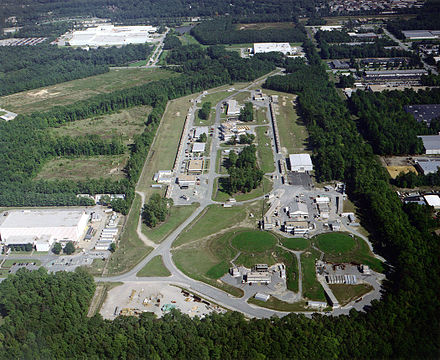
\includegraphics[width=0.8\textwidth]{Chapters/Ch2-Experiment/accel_and_beamline/pics/CEBAF/jlab_wiki.png}
    \caption{An aerial view of the Thomas Jefferson National Accelerator Facility \parencite{Wang2010CEBAFOverview}. Note that this picture was taken before the addition of the fourth detector hall (Hall D).}
    \label{fig:jlab_wiki}
\end{figure}

\subsection{Accelerator Facility}
    
    \figref{fig:jlab_accelerator_layout} shows the overarching scheme of the entire accelerator facility relevant for this experiment. Electrons are produced via the photoelectric effect from a 499 MHz pulsed laser impinges on a Gallium Arsenide photocathode (\figref{fig:gun}). The CEBAF guns operate at 100 kV and accelerate the electrons through a beam chopper (\figref{fig:chopper}) to create the desired beam structure (\figref{fig:structure}) and into the main accelerator circuit, where 1497 MHz superconducting resonator (SRF) cavities provide further acceleration (\figref{fig:klystron}). CEBAF's two $\sim$ 1.1 GV linacs accelerate electrons by consist of 50 cryomodules total, with each cryomodule housing 8 7-cell SRF cavities and the liquid helium necessary to cool them, made possible by JLab's 2K liquid helium refrigerator, the largest in the world as of 2023. The electrons are steered around the curved parts of the track by dipole magnets (\figref{fig:magnets}), making five complete circulations before delivery to the three western experimental halls.
    
    
    \begin{figure}[ht]
        \centering
        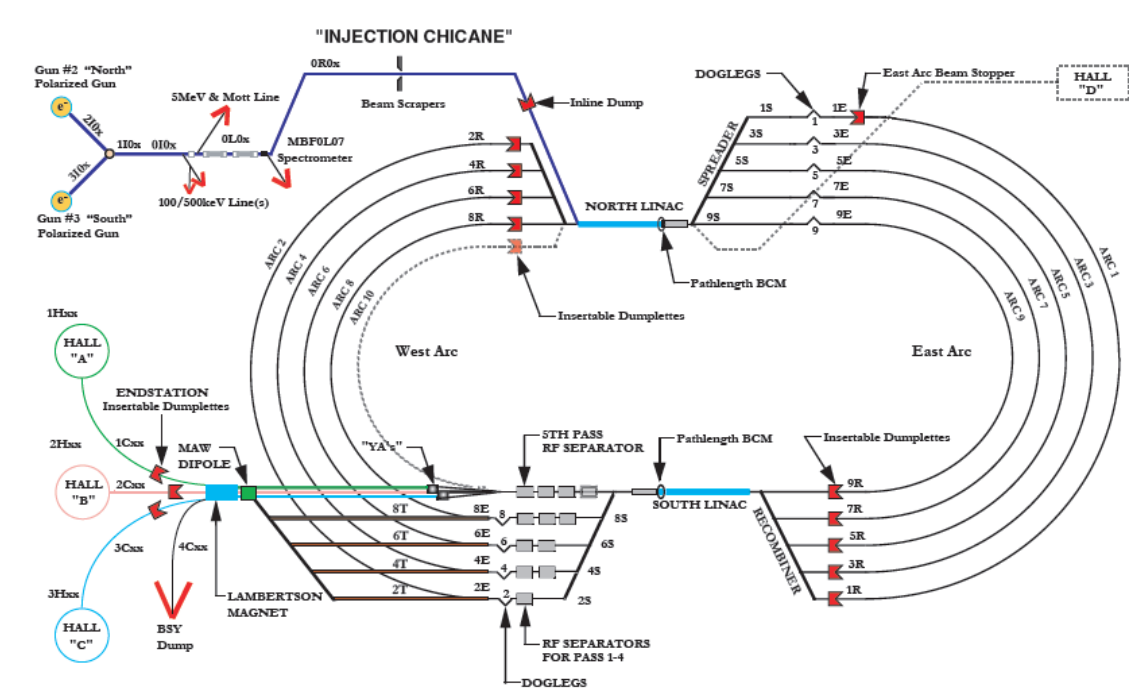
\includegraphics[width=0.8\textwidth]{Chapters/Ch2-Experiment/accel_and_beamline/pics/CEBAF/jlab-accelerator-layout.png}
        \caption{Schematic layout of the CEBAF accelerator at JLab. The racetrack configuration has two linear accelerator portions $\sim$ 1/4 mile long, and is $\sim$ 7/8 mile around \parencite{Wang2010CEBAFOverview}.}
        \label{fig:jlab_accelerator_layout}
    \end{figure}
    
    
    \begin{figure}[htb]
        \begin{minipage}[c]{\linewidth}
            \centering
            \subfloat[]{\label{fig:gun}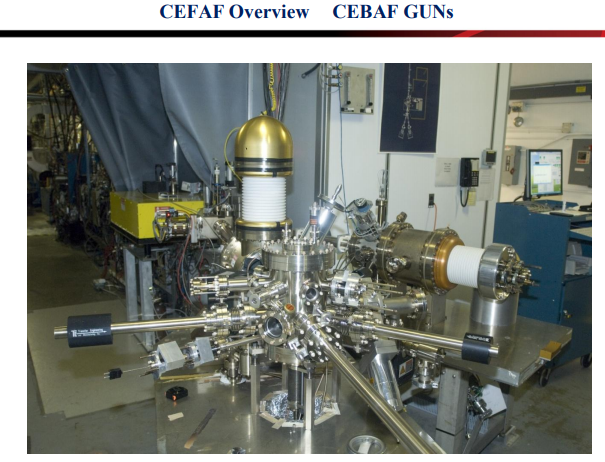
\includegraphics[width=0.3\textwidth]{Chapters/Ch2-Experiment/accel_and_beamline/pics/CEBAF/1_CEBAF-guns.png}}
            \subfloat[]{\label{fig:chopper}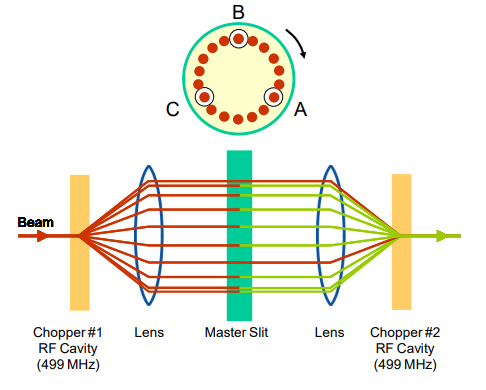
\includegraphics[width=0.3\textwidth]{Chapters/Ch2-Experiment/accel_and_beamline/pics/CEBAF/jlab-chopper.png}}
            \subfloat[]{\label{fig:structure}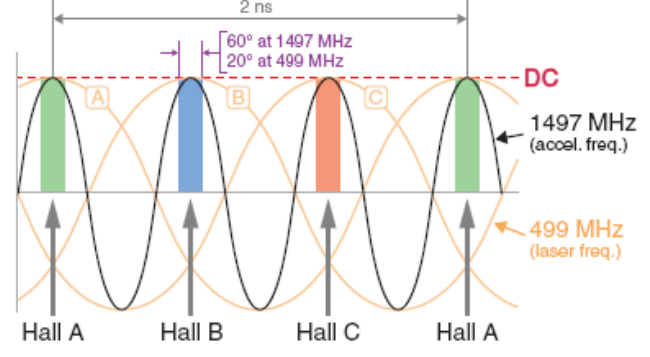
\includegraphics[width=0.3\textwidth]{Chapters/Ch2-Experiment/accel_and_beamline/pics/CEBAF/Jlab-beam-structure.png}}
        \end{minipage}
        \begin{minipage}[c]{\linewidth}
            \centering
            \subfloat[]{\label{fig:klystron}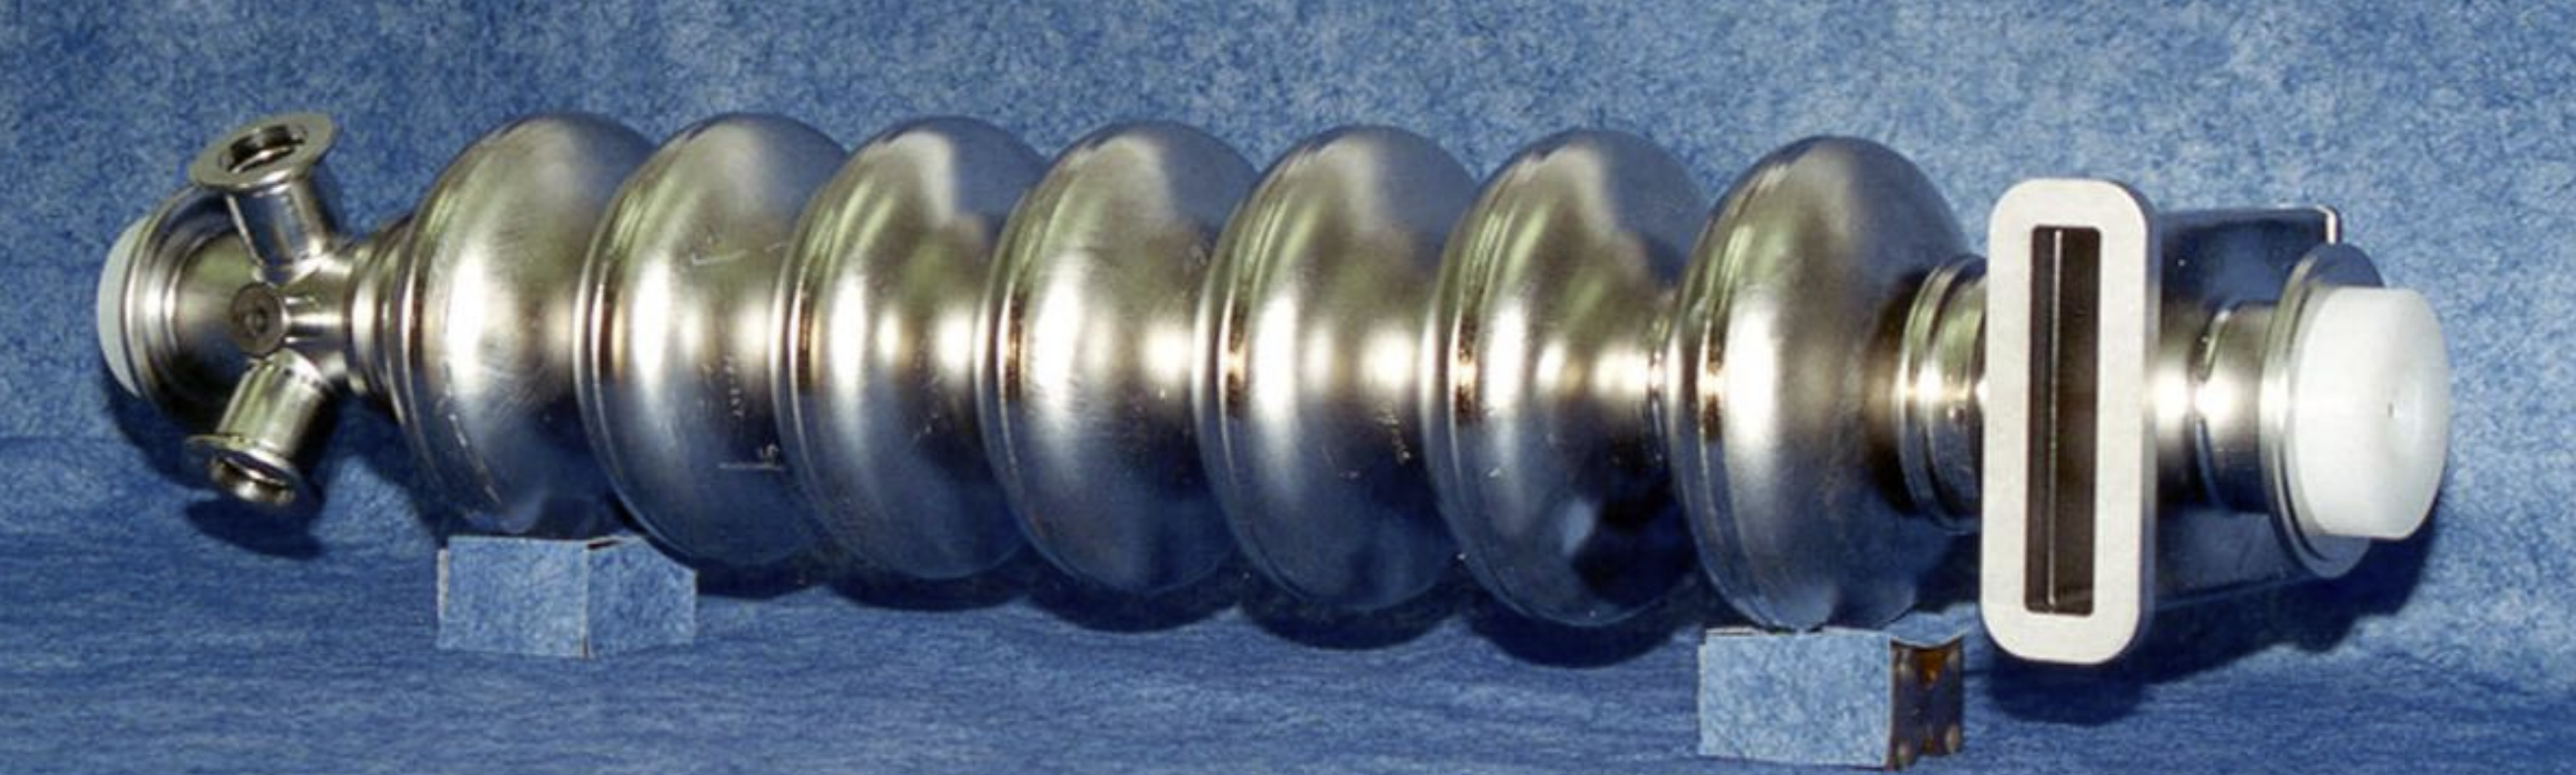
\includegraphics[width=0.4\textwidth]{Chapters/Ch2-Experiment/accel_and_beamline/pics/CEBAF/klystron.png}}
            \subfloat[]{\label{fig:magnets}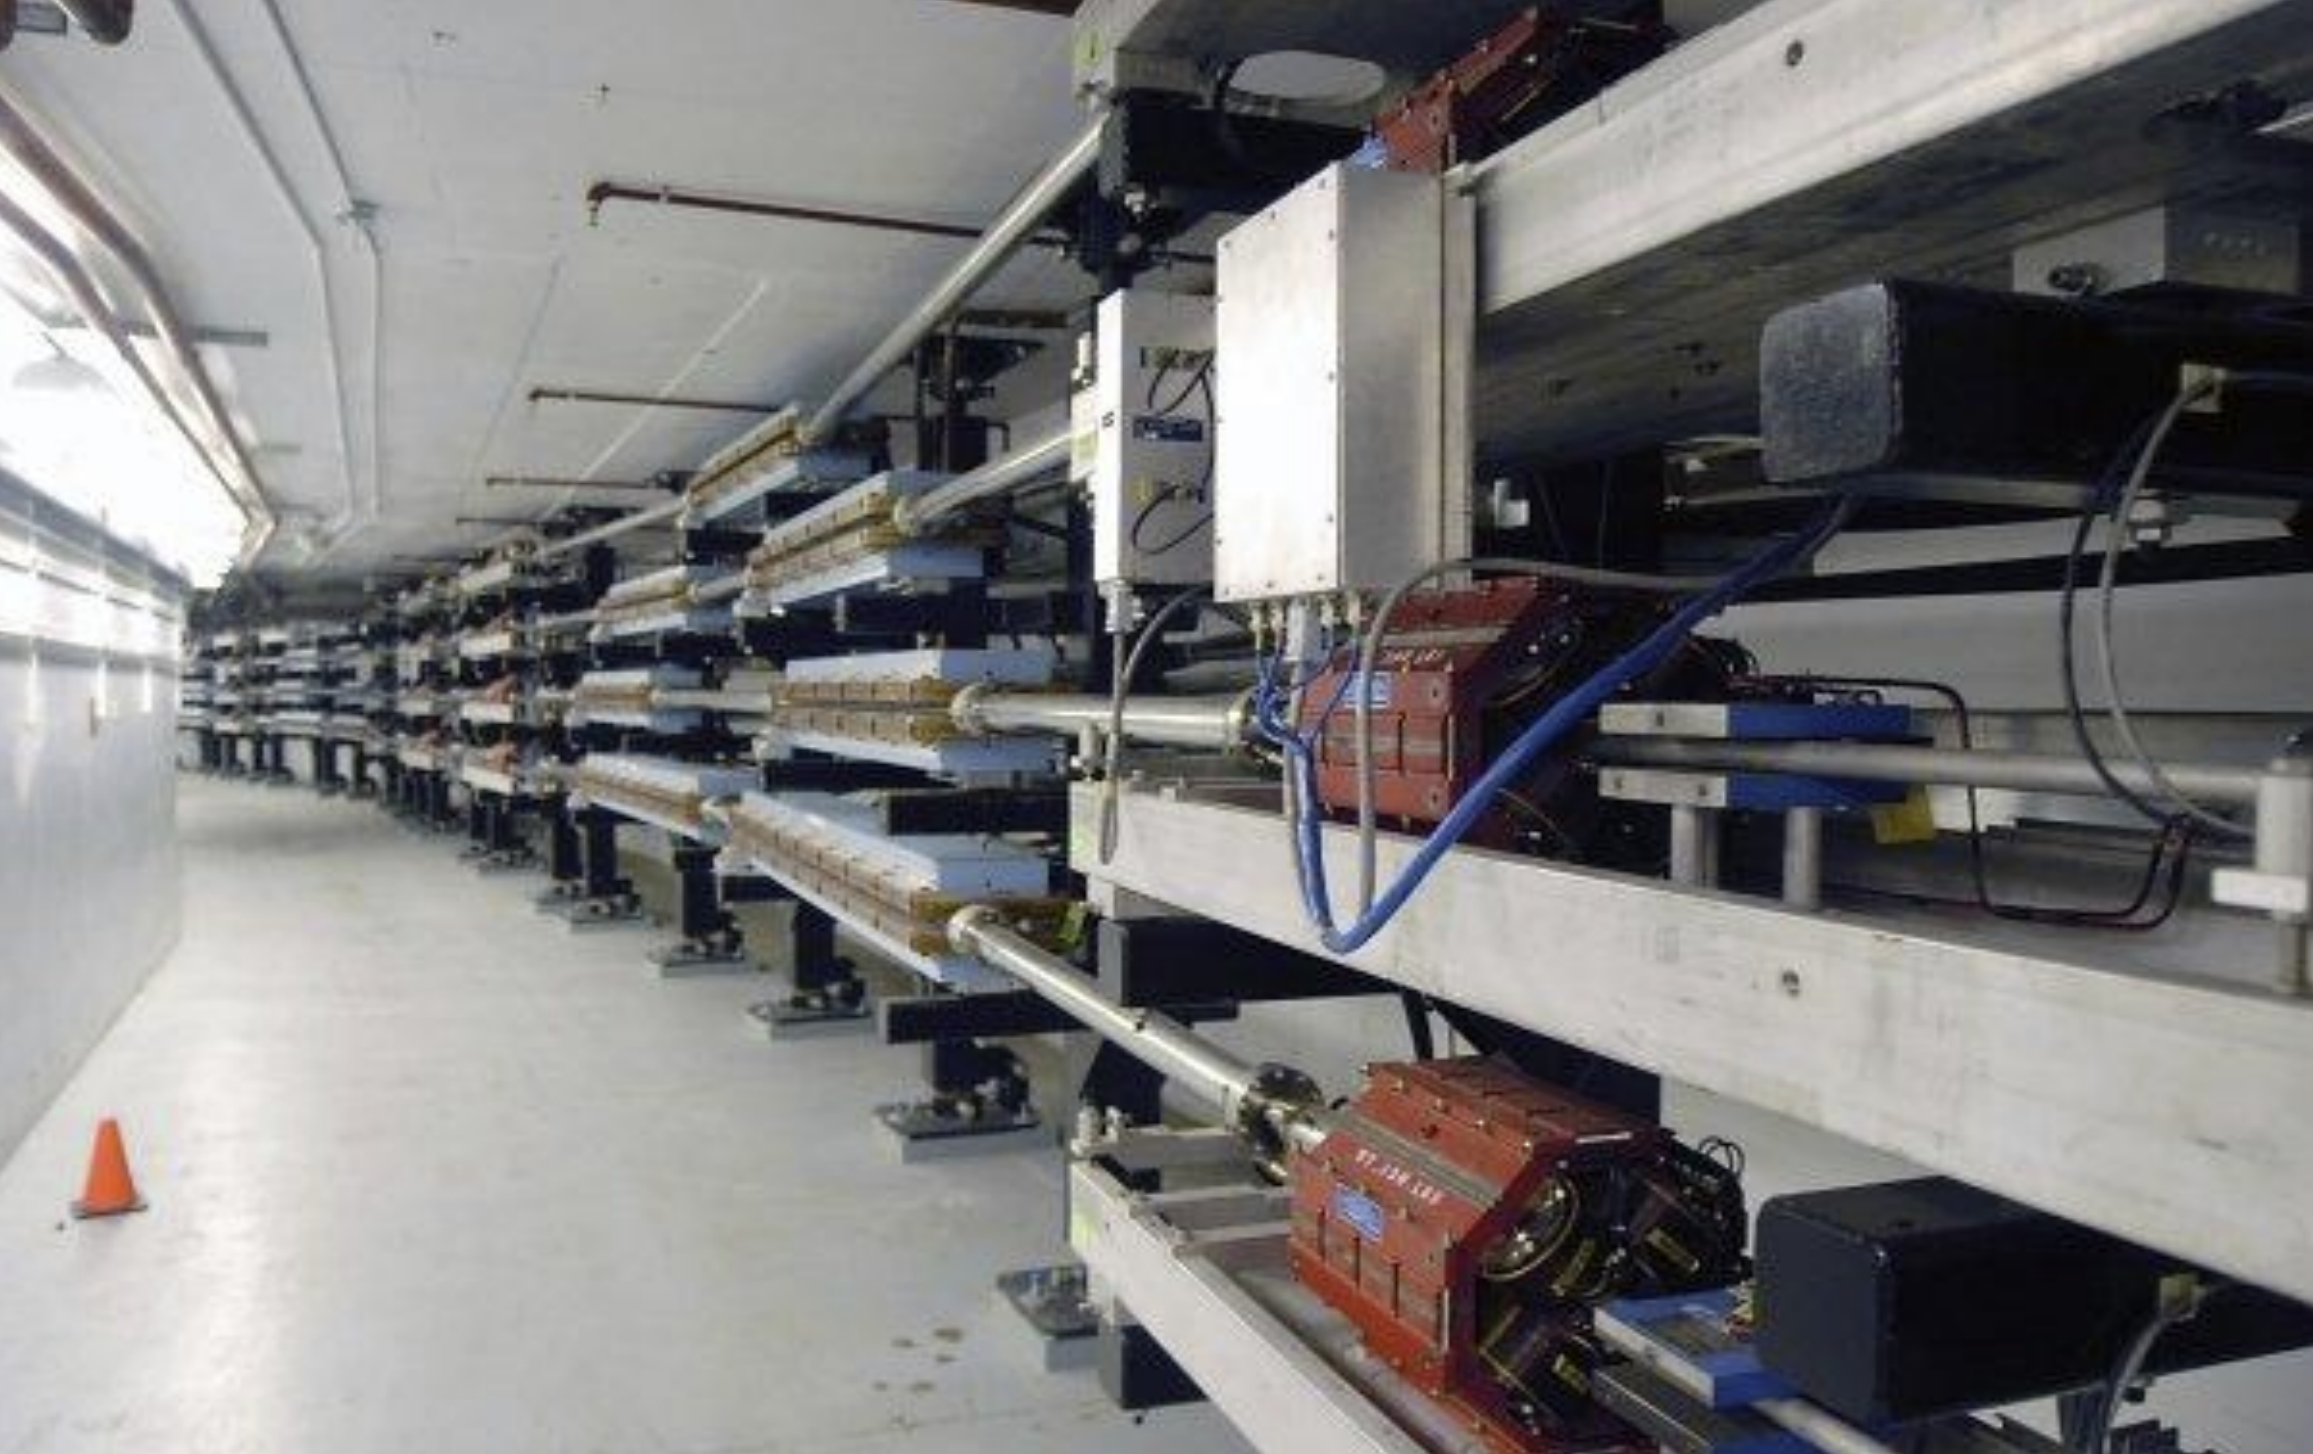
\includegraphics[width=0.4\textwidth]{Chapters/Ch2-Experiment/accel_and_beamline/pics/CEBAF/magnets2.png}}
        \end{minipage}
        \caption{(a) CEBAF guns, (b) Beam chopper, (c) Beam structure, (d) Superconducting resonator, (e) Dipole magnets.}
        \label{fig:JLab}
    \end{figure}
    

\subsection{Hall B Beamline}

    Moller polarimeters
    raster and target
    faraday cup / beamdump

    
    Finally, excess beam is safely managed using beam dumps. 
    
    \begin{figure}[ht]
        \centering
        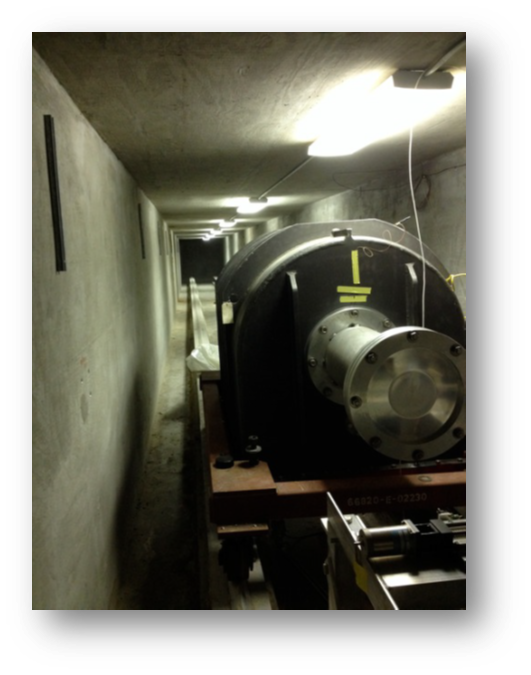
\includegraphics[width=0.8\textwidth]{Chapters/Ch2-Experiment/accel_and_beamline/pics/hallB/beamdump1.png}
        \caption{The first stage of the beam dump system at JLab.}
        \label{fig:beam_dump1}
    \end{figure}
    
    \begin{figure}[ht]
        \centering
        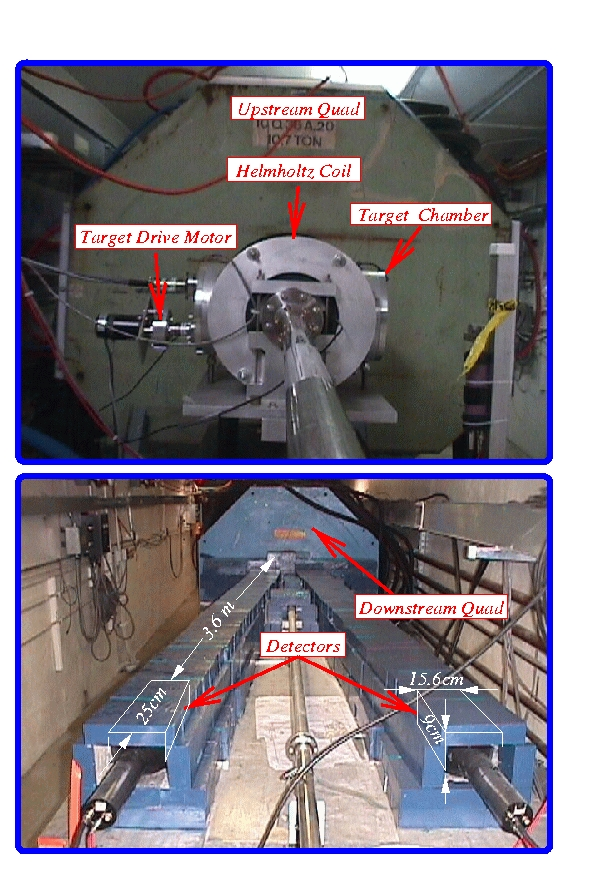
\includegraphics[width=0.8\textwidth]{Chapters/Ch2-Experiment/accel_and_beamline/pics/hallB/hall-b-poll-2.jpg}
        \caption{Moller polarimeters}
        \label{fig:beam_dump1}
    \end{figure}

    
    \begin{figure}[ht]
        \centering
        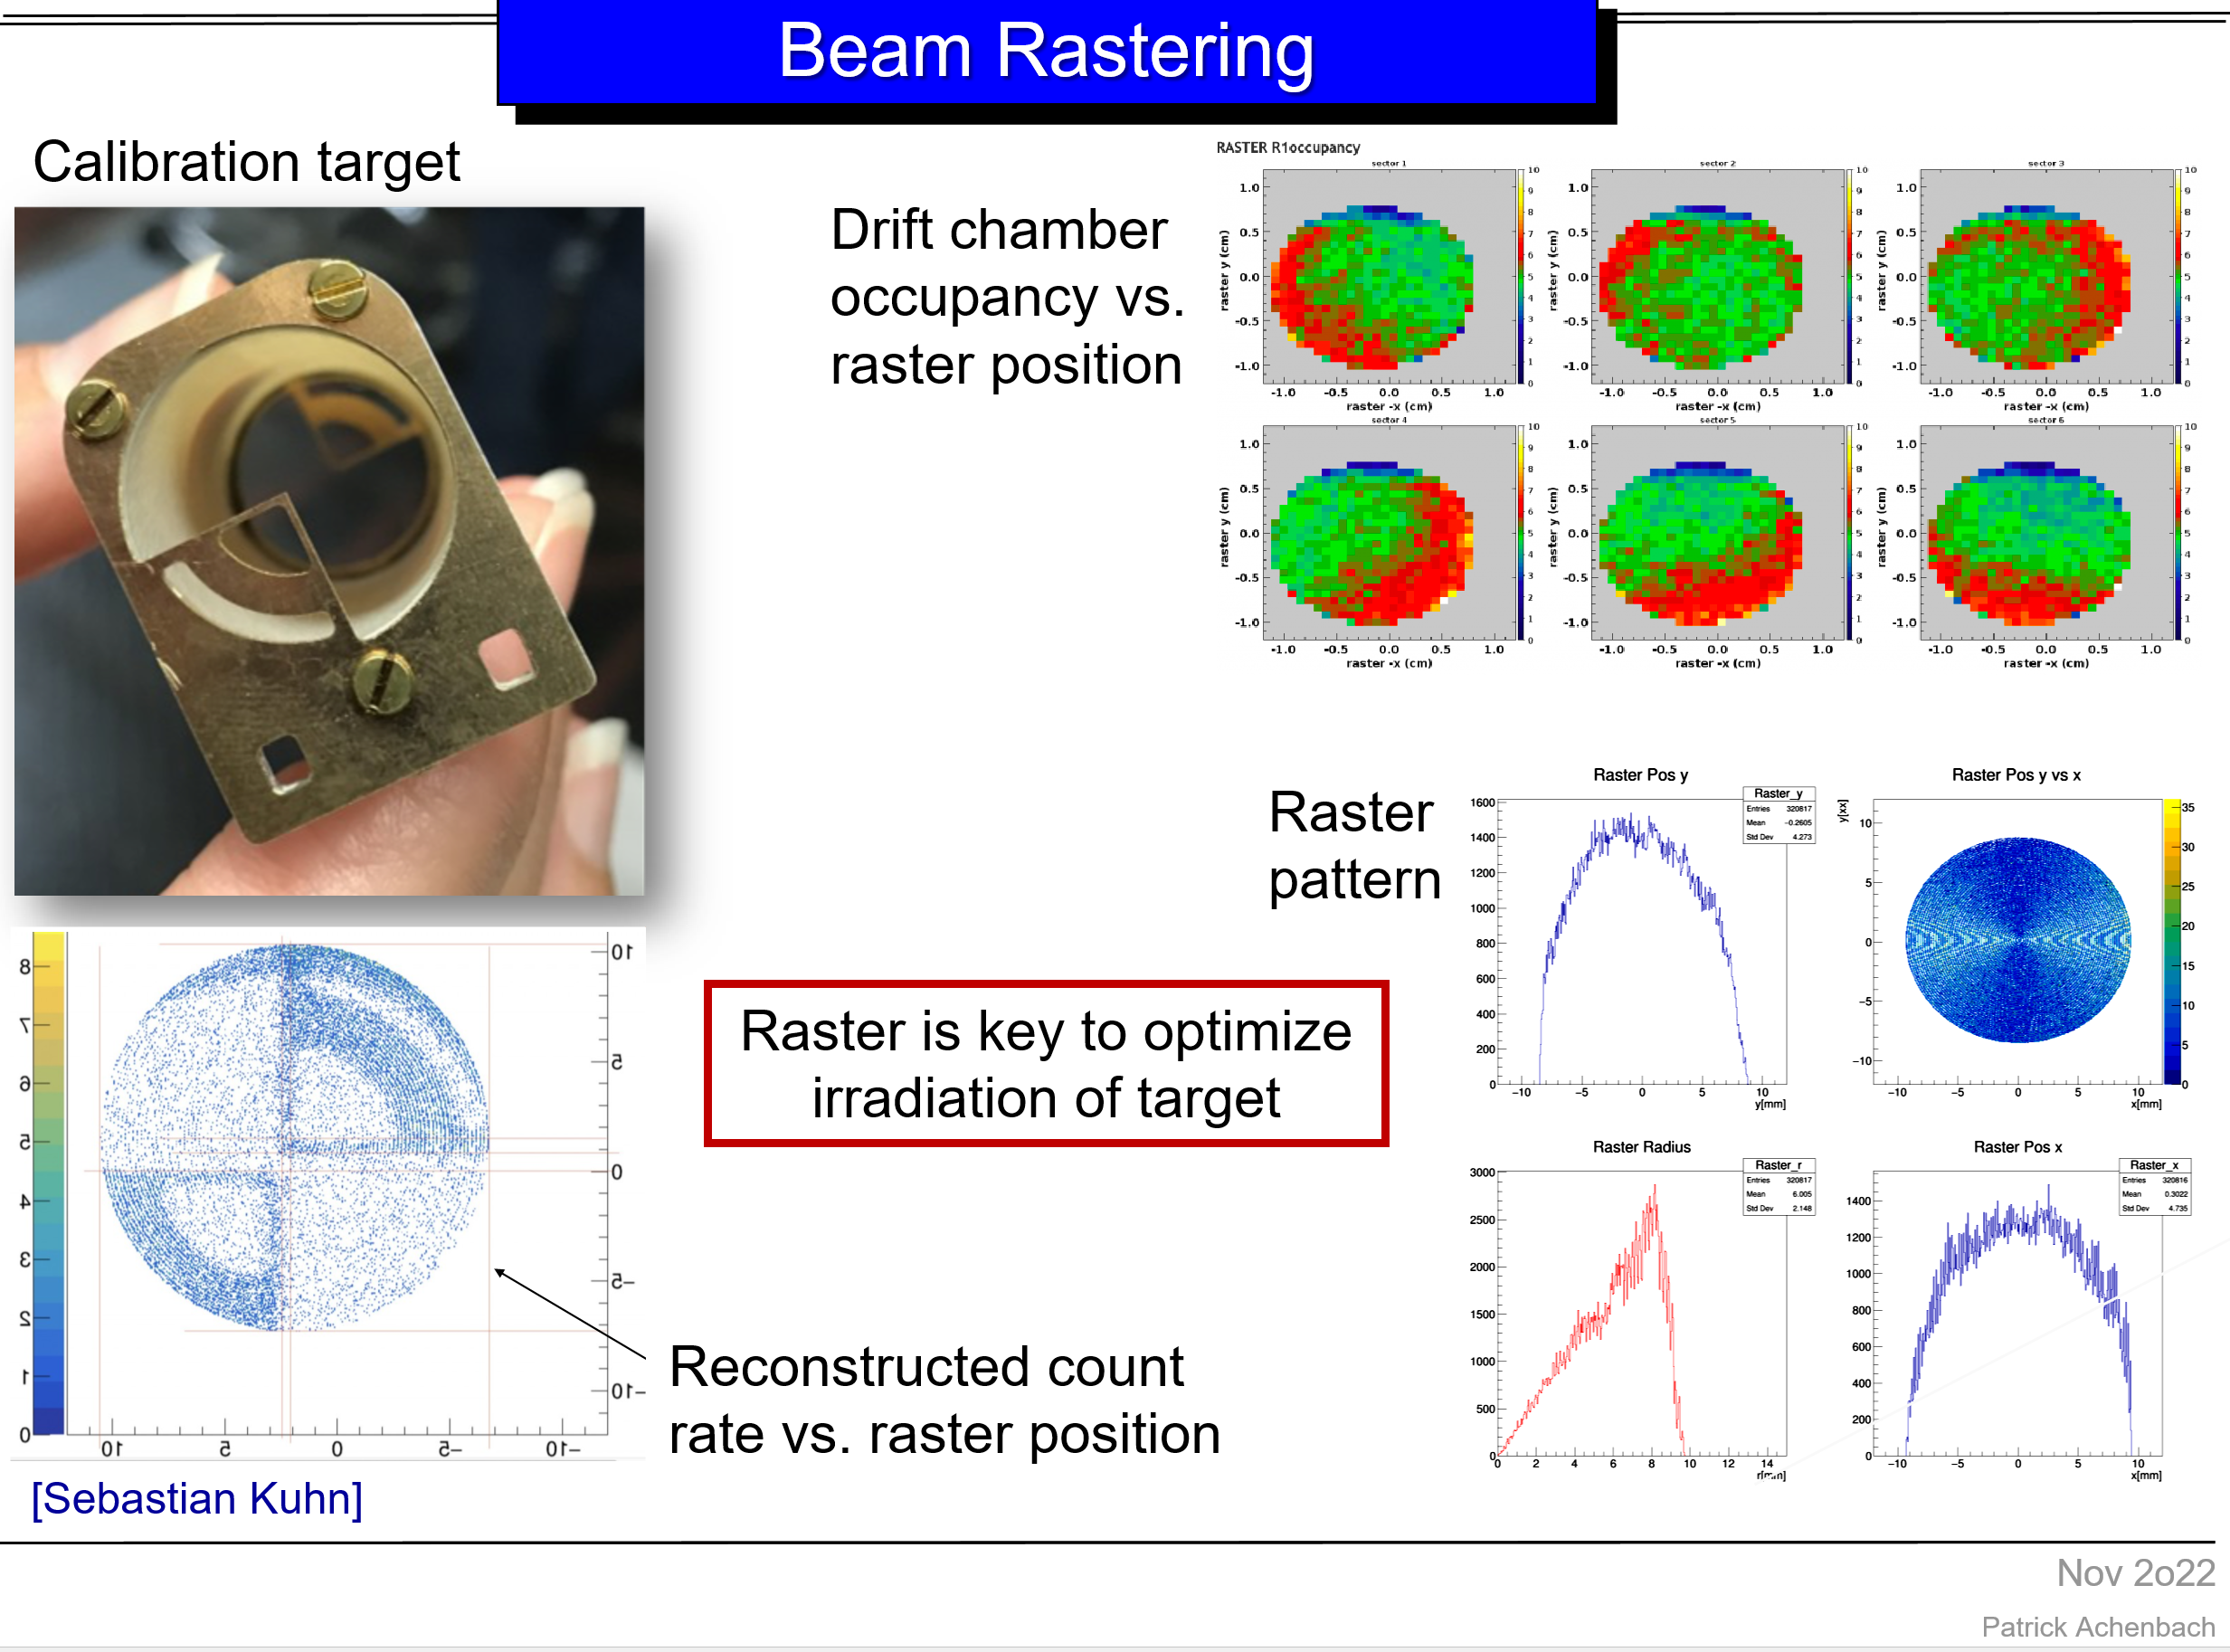
\includegraphics[width=0.8\textwidth]{Chapters/Ch2-Experiment/accel_and_beamline/pics/hallB/beam_rastering.png}
        \caption{The second stage of the beam dump system at JLab.}
        \label{fig:rastering}
    \end{figure}
    
    
    
        in beam dump area, link to own fraday cup paper \cite{Johnston2019RealizationElectrons}
        
    
    For entry into CLAS12, the beamline specs are as follows:\\
                        Beam current: up to 50 nA\\
                        Beam energy spread: $10^-4$\\
                        Beam size: Less than 0.4 mm\\
                        Beam stability: Less than 0.1 mm\\
                        Beam halo: $10^-4$\\
                        Beam polarization: up to 85\%\\
                        
    
    
    
    
    
     As stated, for RGA, the fact that the beam is polarized is not useful, but it is true and is measured by Moller Polarimeters. 
            
                Polarimietry: 
                        Good for beam energies between 100 MeV and 50 GeV. Polarized beam electrons are scat-
                tered from other polarized electrons in a target, usually magnetized foils. Only a small
                fraction of all the target electrons are polarized, so this method has a small analyzing
                power. Analyzing power is exactly calculable in QED. At high beam energies, analyzing
                power and scattering probability both become independently of beam energy. Maximum
                analyzing power is about 80%, maximum is at 90 degrees scattering angle in C.o.M. Trans-
                versely polarized target can be used to measure transverse beam polarization, but analyzing
                power is only about 10%. 90 degrees C.o.M. translates to a small lab angle with each elec-
                tron at half beam energy, so magnets are used to bend these electrons out to detectors.
                These detectors can be, for example lead glass total absorption cherenkov counters.Since
                the two electrons are corellated, can use things like time coincidence to reduce background,
                although for low duty factor accelerators only one electron is required as statistics would
                otherwise be too low.A main background to this process is Mott scattering with the electron
                radiating off energy after scattering, appearing as a Moller electron
                
                The scattering target is either iron or vanadium permendur (iron-cobalt alloy). Only 2 of
                26 electrons in iron have their spins oriented, leading to a total analyzing power of only 6 percent
                and transverse analyzing power of only 1%. Uncertainties in how magnetized the targets
                actually are corresponds to an uncertainty in analyzing power. There are ’easy’ and ’hard’
                magnetization schemes - easy does a soft magnetization, while hard uses a several tesla mag-
                net to saturate the target. In principle, uncertainties on magnetization in the hard scheme
                can be removed by using the Kerr magneto-optic effect, but this has not ever been imple-
                mented. An important correction is due to the Levchuk effect, where due to momentum
                differences between electrons in different shells, electrons scattered off of polarized electrons
                are more likely to be detected than off of unpolarized electrons. Specifically, inner electrons
                are unpolarized and have a large average momenta, so when struck they can fall outside the
                113 TOC
                acceptance of the Moller detectors, while the outer electrons, which are polarized, have a
                small average momentum, and behave as expected. This is up to a 15% effect on polarization
                measurements, and is currently a work in progress.
    
    
                
    
                 Rasterization of some kind
                    \\
                    \indent The hydrogen target in RGA is cooled to 20 K using a He4 evaporation fridge. Can by polarized by dynamic nuclear polarization, driven by a 140 GHz microwave source, can reach 90\% polarization for protons, 40\% for deuterons (both longitudinally polarized). The polarization can be measured by a Q-meter based NMR. 2.5 cm diameter target, extended 5 cm long. \\
                    \indent RGA does not use a polarized target. The beam is polarized, but the target is not, so polarization is not helpful for extracting the 5-fold differential cross section (but it would be if the target was also polarized, and is useful for BSA measurements).
                
       
                Luminosity in CLAS12 is measured from the Faraday Cup and using reference reactions such as elastic scattering. We don't use the Faraday Cup event by event, but we do use it run by run. For beam current measurements, beam position monitors upstream are used - but this is for monitoring on-line, not for analysis.
                           Can manage 175 Watts - 17 nA at 10 GeV. Is used to calibrate beam current, needs a blocker in at higher currents

\cleardoublepage
                                         

\section{CLAS Detectors and Run Conditions}\label{sec:clas12exp}
    The CEBAF Large Acceptance Spectrometer, 12 GeV (CLAS12) detector occupies experimental Hall B at Jefferson Lab. It is an upgrade from its predecessor, the CLAS detector \parencite{Mecking2003TheCLAS}, which operated in the 2000s during the 6 GeV era of JLab and laid the groundwork for the present detector system, which was commissioned in 2018. It covers nearly 4$\pi$ around the target cell, with comprehensive packages of detectors for particle position and energy tracking. It operates with data rates of comparable size to other large-scale, international physics experiments, as shown in \tabref{table:experiments}. Data taking began in 2018 and has an experimental program approved into at least the early 2030s \parencite{Battaglieri2021PresentProgram}.

\iffalse
%Differences between clas and clas12 detectors
CLAS12 acceptances and resolutions are also superior to that of CLAS6. Main differences are:
- RGK has outbending torus vs inbending CLAS6 data
- the distance between the target and the PCal has increased, the FTCal extends to lower angles, and the gap between FTCal and PCal is much smaller than between IC and EC
- proton polar angle was limited to 60 deg in the e1dvcs dataset if my memory is correct
\fi


\begin{table}[h]
    \centering
    \begin{tabular}{l|lccc}
         \headercell{\textbf{Facility}} & \textbf{Experiment} &  \headercell{\textbf{Event Size} \\ \textbf{(kB)}}  &  \headercell{\textbf{L1 Trigger Rate} \\ \textbf{(kHz)}}  &  \headercell{\textbf{Bandwidth to Storage} \\ \textbf{(MB/s)}}      \\ \\ \hline
        JLab & GlueX & 15 & 200 & 300 \\
        JLab & \textcolor{purple}{\textbf{CLAS12}} & \textcolor{purple}{\textbf{20}} & \textcolor{purple}{\textbf{10}} & \textcolor{purple}{\textbf{100}} \\
        LHC & ALICE & 2,500 & 200 & 200 \\
        LHC & ATLAS & 1,500 & 75 & 300 \\
        LHC & CMS & 1,000 & 100 & 100 \\
        LHC & LHCb & 40 & 1,000 & 100 \\
        BNL & STAR & 1,000 & 0.6 & 450 \\
        BNL & PHENIX & 60 & 15 & 450 \\
    \end{tabular}
\caption[Data rates of various physics experiments]{Assorted physics experiments and their typical data rates. Note that exact figures vary by source and run conditions. Adapted from \parencite{DavidLawrence2012TheLab}.}
\label{table:experiments}
\end{table}

\subsection{CLAS12 Detector System}
    The CLAS12 detector \figref{fig:clas12photo} has two major subsystems: the Forward Detector and the Central Detector, as well as a forward tagger (nested inside the forward detector package) and backward angle neutron detector (BAND). 



\begin{figure}[H]
    \centering
    \subfloat[CLAS12 CAD layout.]{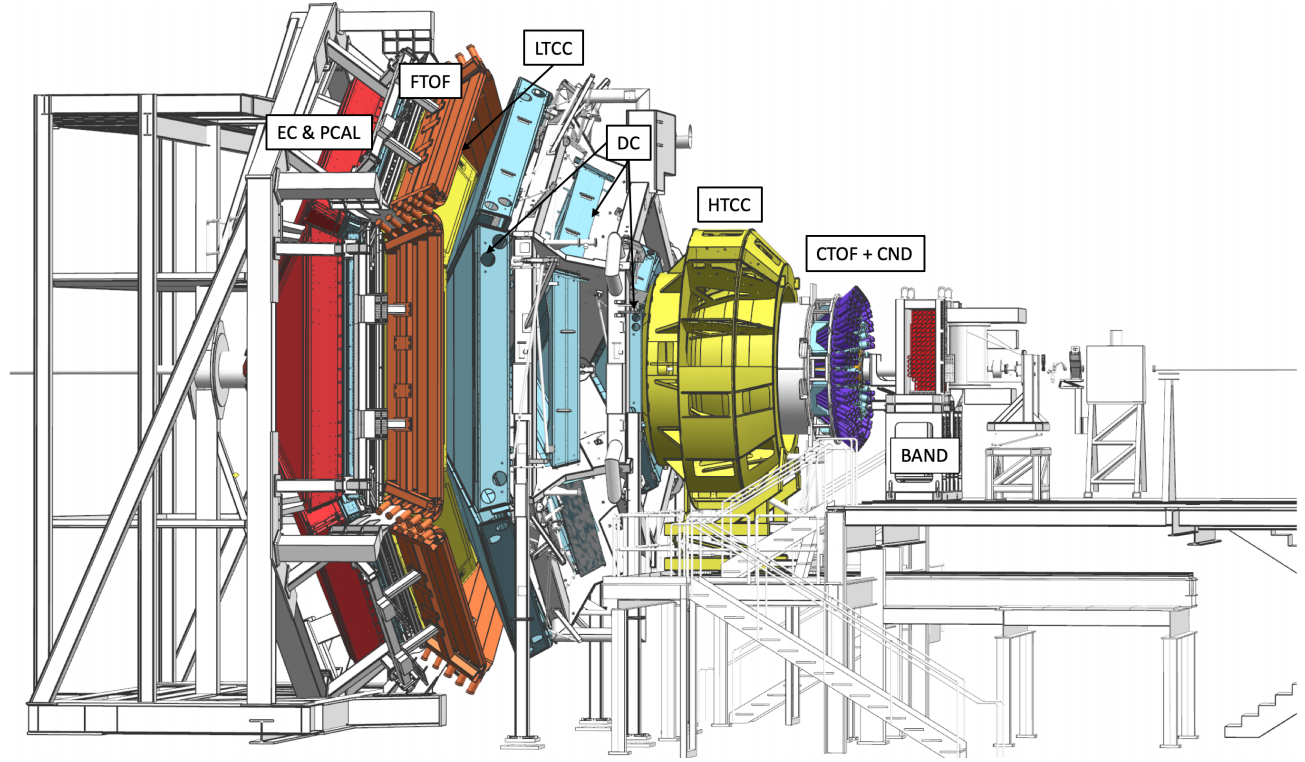
\includegraphics[width=0.45\textwidth]{Chapters/Ch2-Experiment/clas-12-exp/clas-detectors/other/pics/CLAS12.png}\label{fig:clas12}}
    \hfill
    \subfloat[CLAS12, fully installed.]{\includegraphics[width=0.45\textwidth]{Chapters/Ch2-Experiment/clas-12-exp/clas-detectors/other/pics/clas-real.png}\label{fig:clas12spec}}
    \caption[CLAS12 Layout]{CLAS12 layout schematic and photograph, from \parencite{Burkert2020TheLaboratory}.}\label{fig:clas12photo}
\end{figure}



\subsubsection*{Forward Detector}

    The Forward Detector (FD) is a 6-fold azimuthally symmetric segmented system containing several detector packages and a toroidal magnet. The sections follow a counterclockwise numbering convention where S1 corresponds to $[-30^{\circ}, 30^{\circ}]$, as in \figref{fig:fd_sections}. Working from the target downstream, the FD consists of a High Threshold Cherenkov Counter (HTCC) \parencite{Sharabian2020TheCounter}, Low Threshold Cherenkov Counter (LTCC) \parencite{Ungaro2020TheDetector}, the Ring Imaging Cherenkov detector (RICH) \parencite{Contalbrigo2020TheDetector}, Forward Time-of-Flight (FTOF) \parencite{Carman2020TheSystem}, Drift Chambers (DC) \parencite{Mestayer2020TheSystem} embedded in a 3.5 Tesla torodial magnetic field \parencite{Fair2020TheMagnets}, and Electromagnetic Calorimeter (ECal) complex \parencite{Asryan2020TheCalorimeter}.

    The ECal consists of three layers, two of which are from the previous CLAS experiment \parencite{Amarian2001TheCalorimeter}. Those two layers were only sufficient to contain showers with energies below 5 GeV, so a third layer (Pre-shower Calorimeter, PCal) was added to address this issue, as well as introduce the finer grained segmentation necessary to resolve the angle between the two photons of a neutral pion decay, which is of special importance for this process measurement. The FD system covers approximately $5^{\circ}$ to $35^{\circ}$ in polar angle, with one layer of the FTOF (FTOF-2) extending coverage to $45^{\circ}$. 
    
    %Likewise, the FTOF has three layers---FTOF 1a, FTOF 1b, and FTOF 2. The LTCC and the RICH were not used in this measurement.
               
    \begin{figure}[H]
        \centering
        \subfloat[FD sectioning.]{
            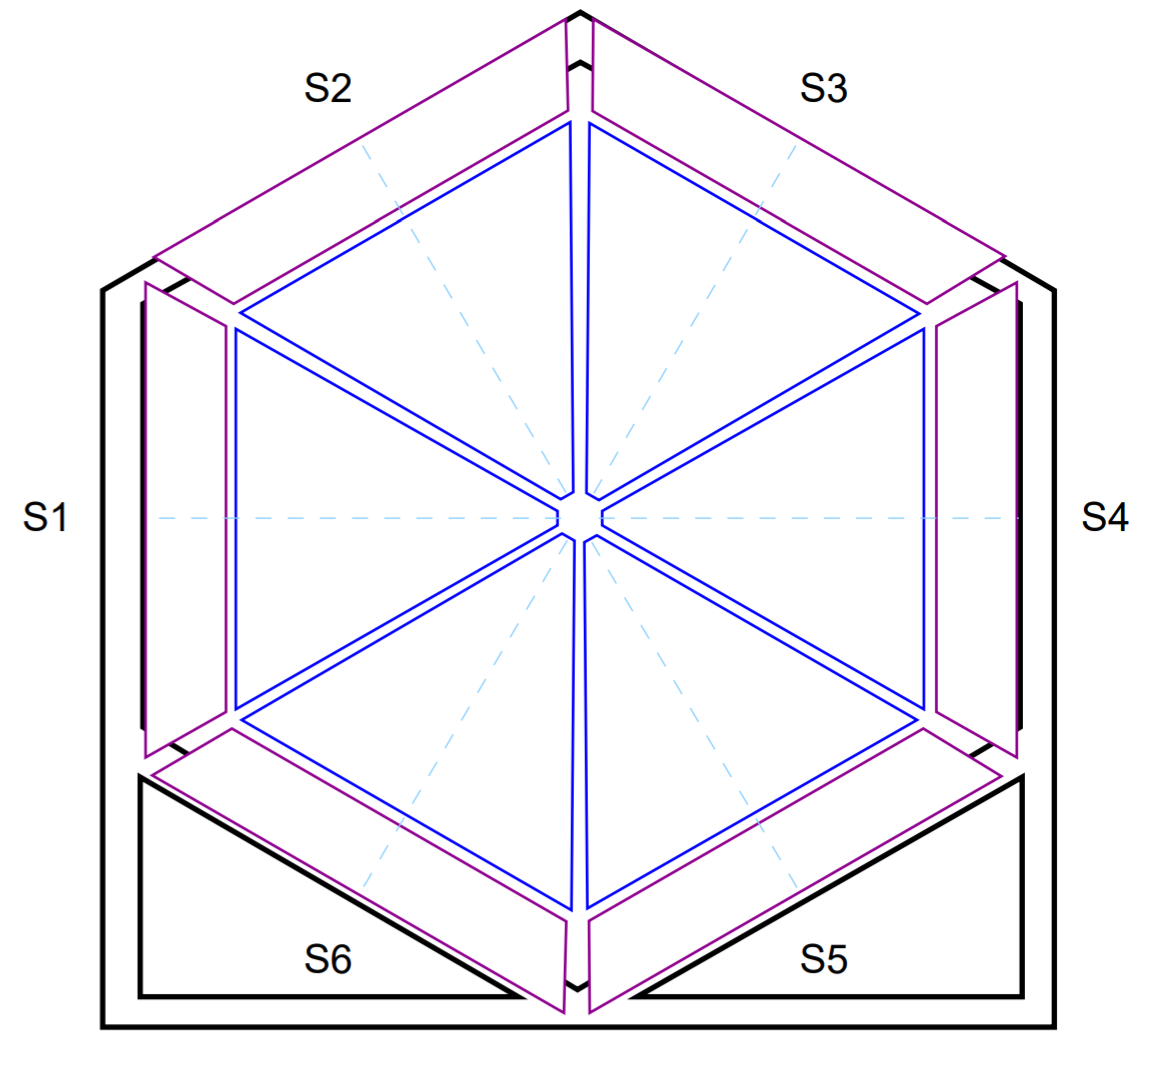
\includegraphics[width=0.3\textwidth]{Chapters/Ch2-Experiment/clas-12-exp/clas-detectors/fd/pics/ftof-front.png}\label{fig:fd_sections}
        }
        \hfill
        \subfloat[Model of HTCC.]{
            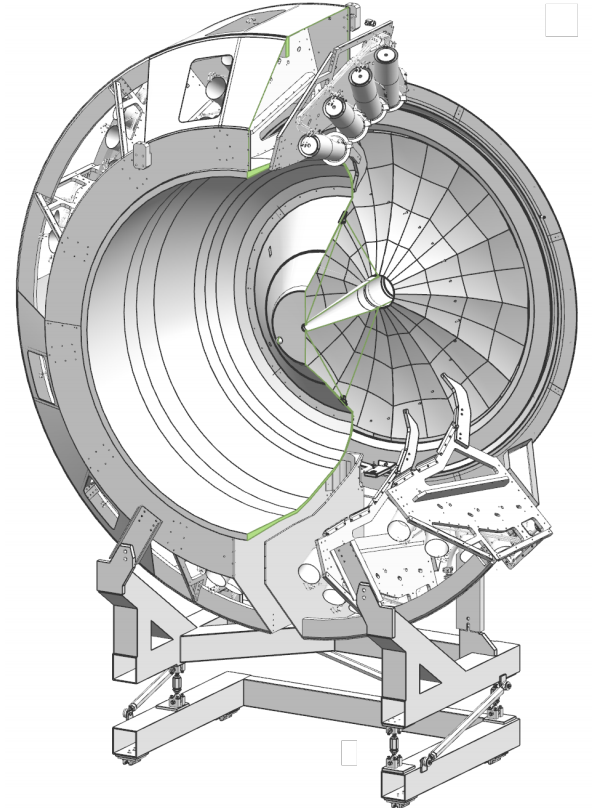
\includegraphics[width=0.3\textwidth]{Chapters/Ch2-Experiment/clas-12-exp/clas-detectors/fd/pics/htcc.png}\label{fig:htcc}
        }
        \hfill
         \subfloat[PCal and ECal assembly.]{
            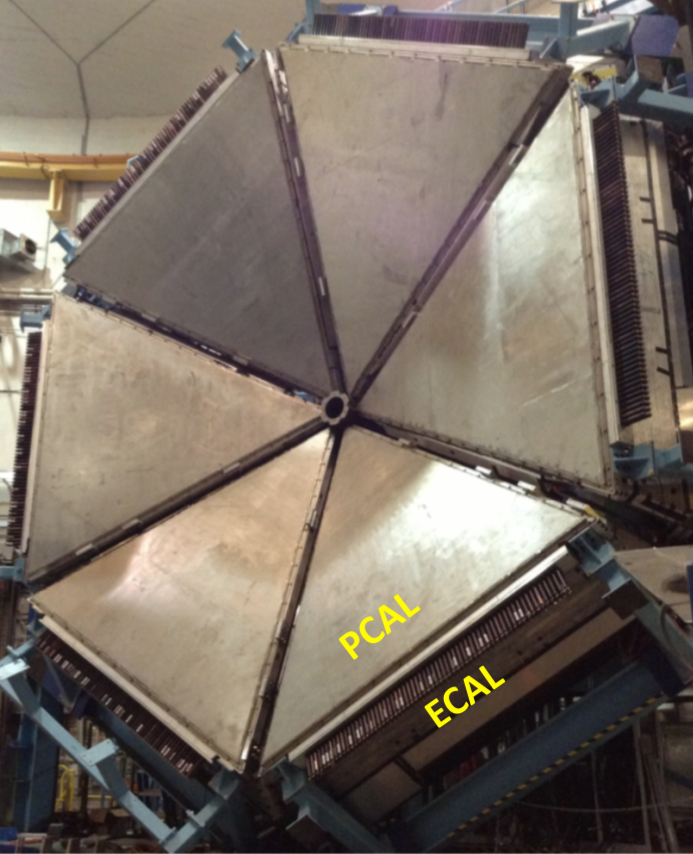
\includegraphics[width=0.3\textwidth]{Chapters/Ch2-Experiment/clas-12-exp/clas-detectors/fd/pics/clas12-pcal-ecal.png}\label{fig:pcalecal}
        }
        \caption[Forward Detector Packages]{The FD is broken into six sections (a), with the exception of the first component after the target, the HTCC (b). The PCal was added to the ECal from the CLAS experiment to achieve the necessary particle resolution. From \parencite{Burkert2020TheLaboratory}}
        \label{fig:select_FD_components}
    \end{figure}




\subsubsection*{Central Detector}

    The Central Detector (CD) also provides nearly 2$\pi$ azimuthal coverage, and spans from $\sim$ $35^{\circ}$  to $125^{\circ}$ in polar angle. The CD is an approximately 1 meter long cylinder inside a 5 Tesla solenoidal magnet \parencite{Fair2020TheMagnets} with four sub-detector packages. From the target working out, the packages are a Central Vertex Tracker \figref{fig:mvt}, made of a Barrel Micromegas Tracker (BMT) \parencite{Acker2020TheTracker} and Silicon Vertex Tracker (SVT) \parencite{Antonioli2020TheTracker}, a Central Time-of-Flight (CTOF) \parencite{Carman2020TheSystem} \ref{fig:ctof}, and a Central Neutron Detector (CND) \parencite{Chatagnon2020TheDetector}, which was installed but not used in this measurement. 
    
    %The main part is the SVT, while the BMT is used to improve the track reconstruction. 

    Low momentum transfer t \eqref{eq:t_momentum_trans} events correspond to large proton polar angles, meaning the majority of low-t events occur with a proton detected in the CD. These events are important as the GPD interpretation of deeply virtual processes is only valid in the regime where $\frac{-t}{Q^2}$ is small, and as such the CD is invaluable to acquiring data to gain insight on these distributions.        


        %CTOF
        %    Central for PID purposes. Divides into 48 1 meter long plastic scintillators with double sided PMT readout.PMTs are in the 0.1 T fringe field region and enclosed in magnetic shielding. 65 picosecond timing resolution. 35 to 125 degrees, 2 $\pi$ in polar angle. 3 cm x 3 cm scintillator planks. Pion/Kaon separation up to 0.64 GeV, Kaon/proton separation up to 1 GeV, pion proton separation up to 1.25 GeV.  	

 
        
        %Solenoid
	%	    5 Tesla super conducting magnet, uniform field ($\Delta$B/B = $10^-4$). Weakest at small angles, strongest at large angles. Opening polar angle of 40 degrees. Momentum range of interest 0.3 to 1.3 GeV. 18 Megajoules stored energy. 85 cm in diameter, 4.2 Kelvin operation. 


        \begin{figure}[H]
            \centering
            \subfloat[Model of CTOF.]{
                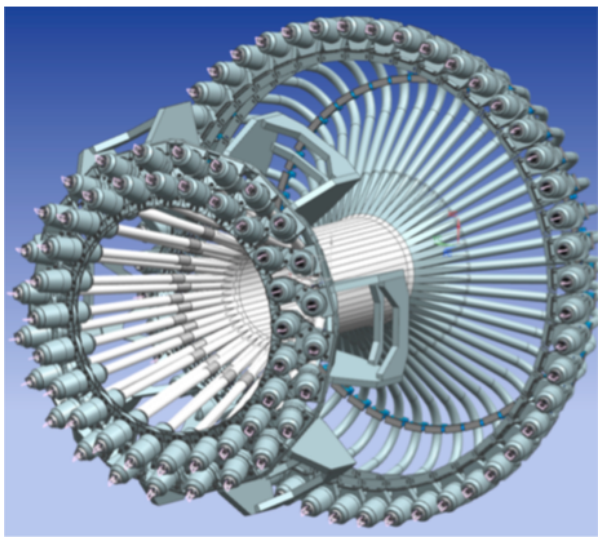
\includegraphics[width=0.3\textwidth]{Chapters/Ch2-Experiment/clas-12-exp/clas-detectors/cd/pics/CTOF.png}\label{fig:ctof}
            }
            \hfill
            \subfloat[Schematic of CVT.]{
                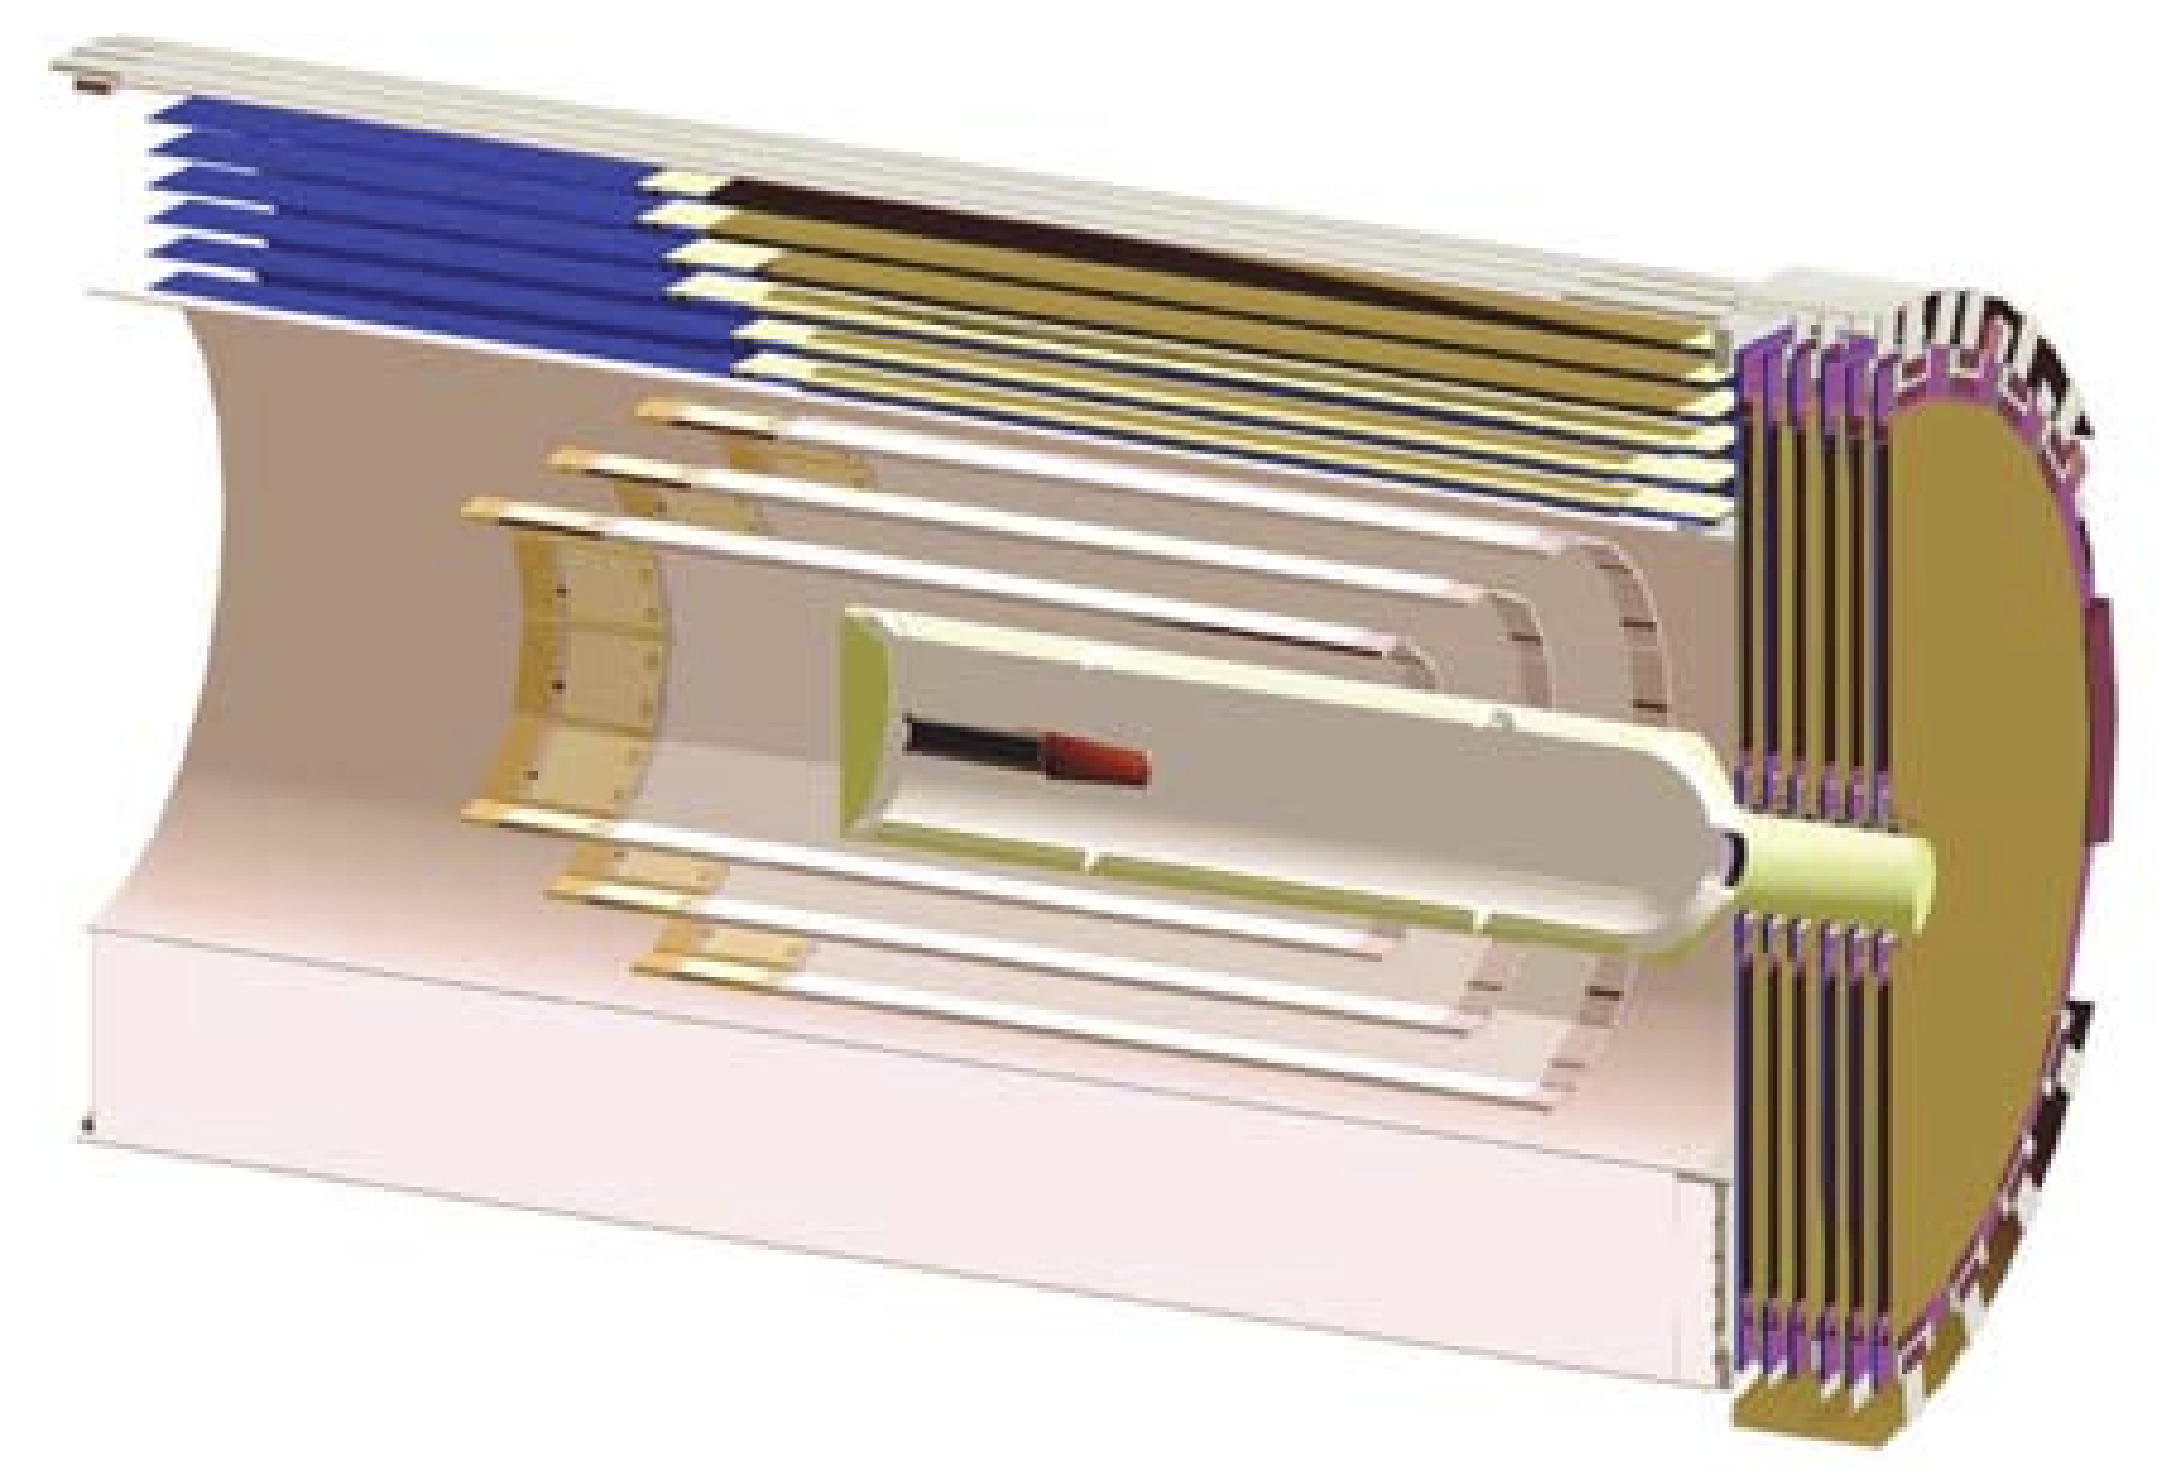
\includegraphics[width=0.3\textwidth]{Chapters/Ch2-Experiment/clas-12-exp/clas-detectors/cd/pics/CVT.png}\label{fig:mvt}
            }
            \hfill
            \subfloat[The CD, in retracted position for maintenance.]{
                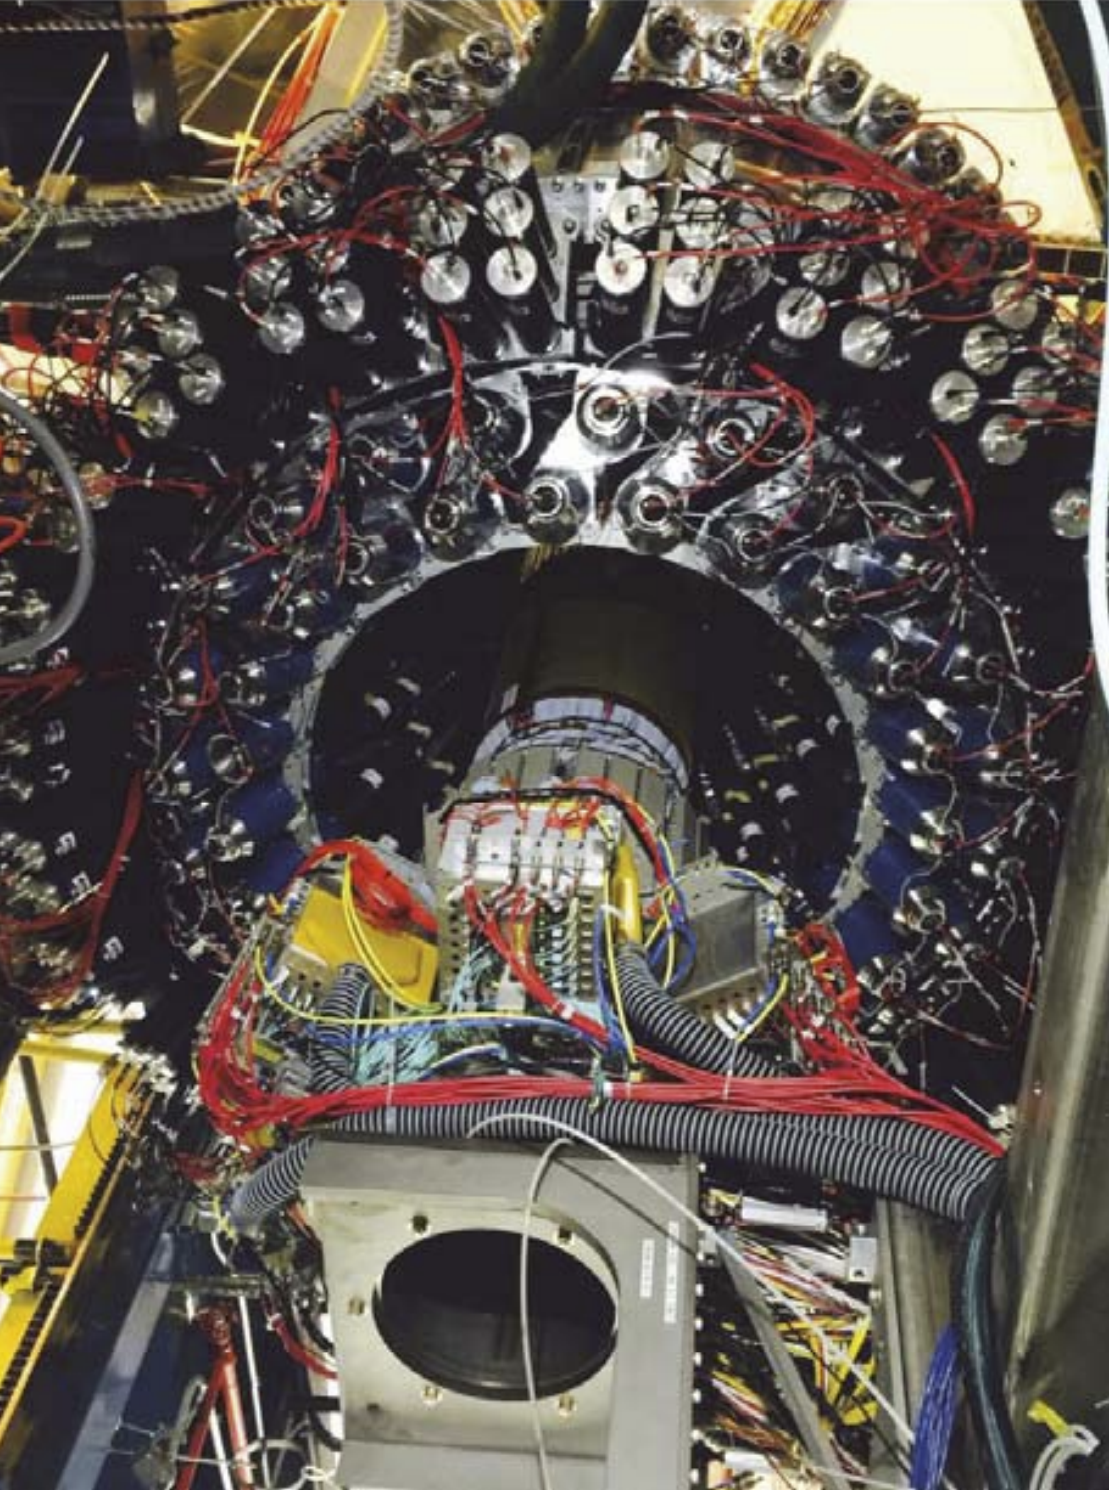
\includegraphics[trim={0 5cm 0 0},clip,width=0.3\textwidth]{Chapters/Ch2-Experiment/clas-12-exp/clas-detectors/cd/pics/real_CD.png}
            }
            \caption[Central Detector Packages]{Models of the CTOF (a) and CVT (b) and their physical realizations in the CD (c). Note the first three inner cylindrical layers of the CVT (b) correspond to the SVT, the outer six to the BMT, and the right end cap six to the FMT. Images from \parencite{Burkert2020TheLaboratory}.}
            \label{fig:your_labels}
        \end{figure}
     
        

\subsubsection*{Other System Components}

    At very low beam angles ($2.5^{\circ}$-$4.5^{\circ}$) there is the Forward Tagger (FT) \parencite{Acker2020TheTagger} which contains a tracker, homogeneous calorimeter, and hodoscope. At the other end of the beamline ($155^{\circ}$-$175^{\circ}$) there is the Backward Angle Neutron Detector (BAND)  \parencite{Segarra2020TheBAND}, which is not relevant for this analysis. Furthermore, the BAND and the Forward Micromegas Tracker (FMT)  \parencite{Acker2020TheTracker} were not installed at the time the data for this analysis was taken, although they have since been commissioned. 
    
    

\iffalse
%To possibly encorporate

    \begin{figure}[H]
        \centering
        \subfloat[]{
            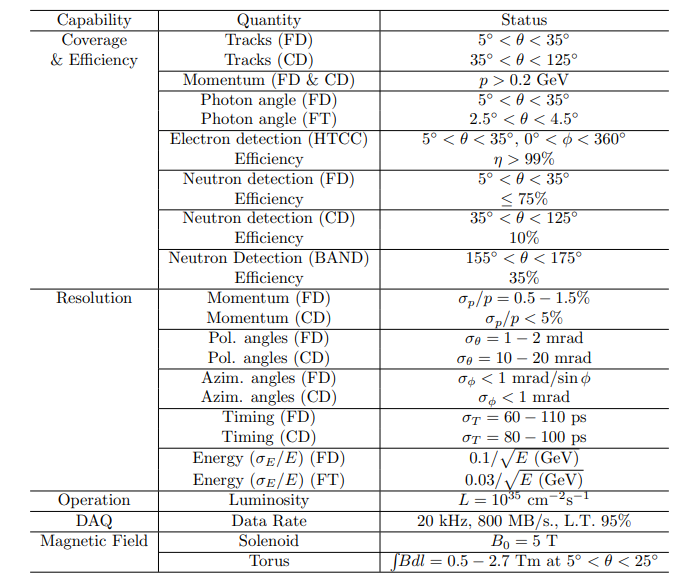
\includegraphics[width=0.3\textwidth]{Chapters/Ch2-Experiment/clas-12-exp/clas-detectors/other/pics/clas12-params.png}
        }
        \hfill
        \subfloat[]{
            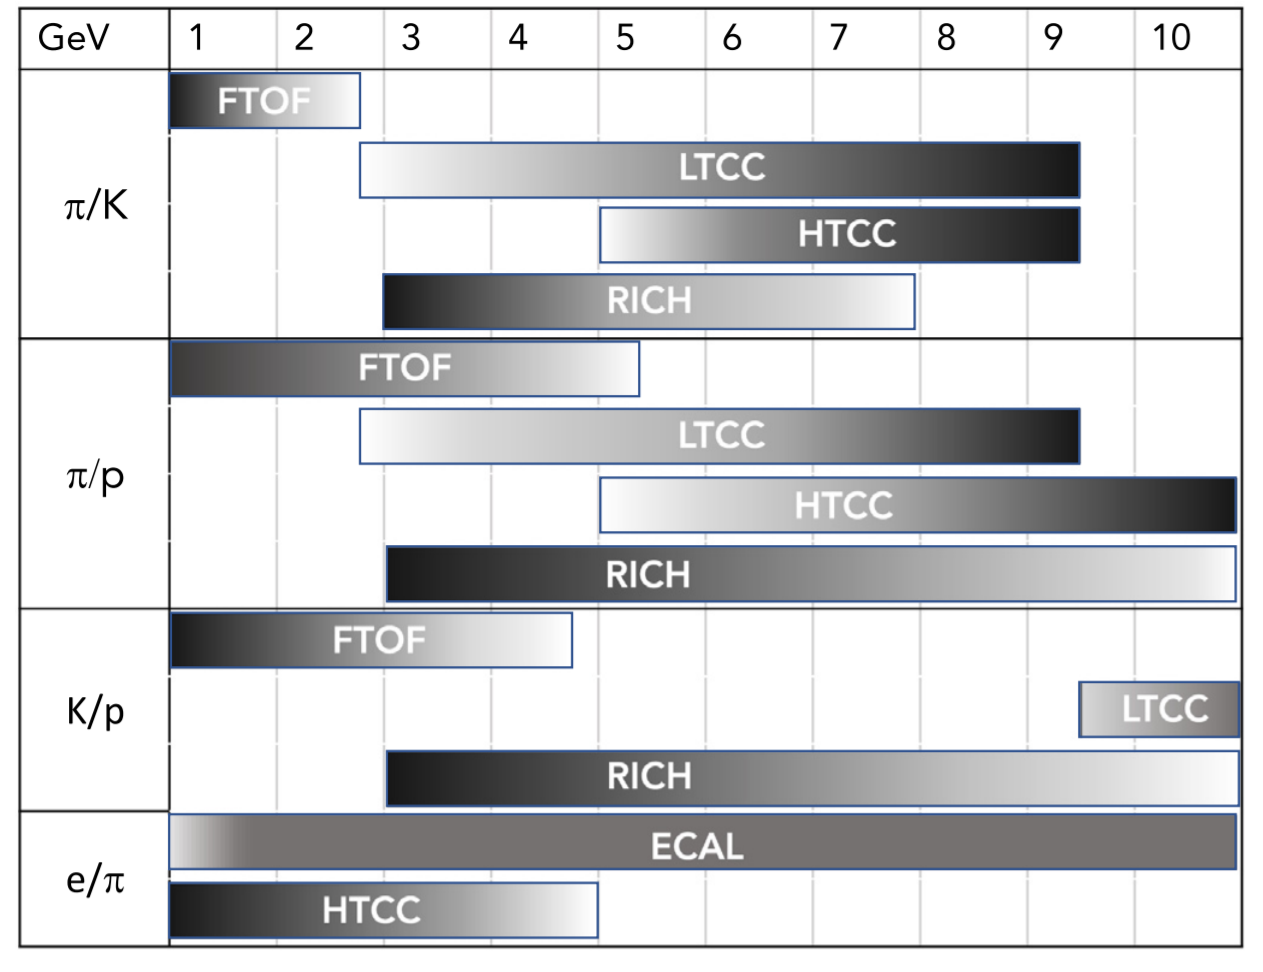
\includegraphics[width=0.3\textwidth]{Chapters/Ch2-Experiment/clas-12-exp/clas-detectors/other/pics/pid-clas12.png}
        }
        \hfill
        \subfloat[]{
            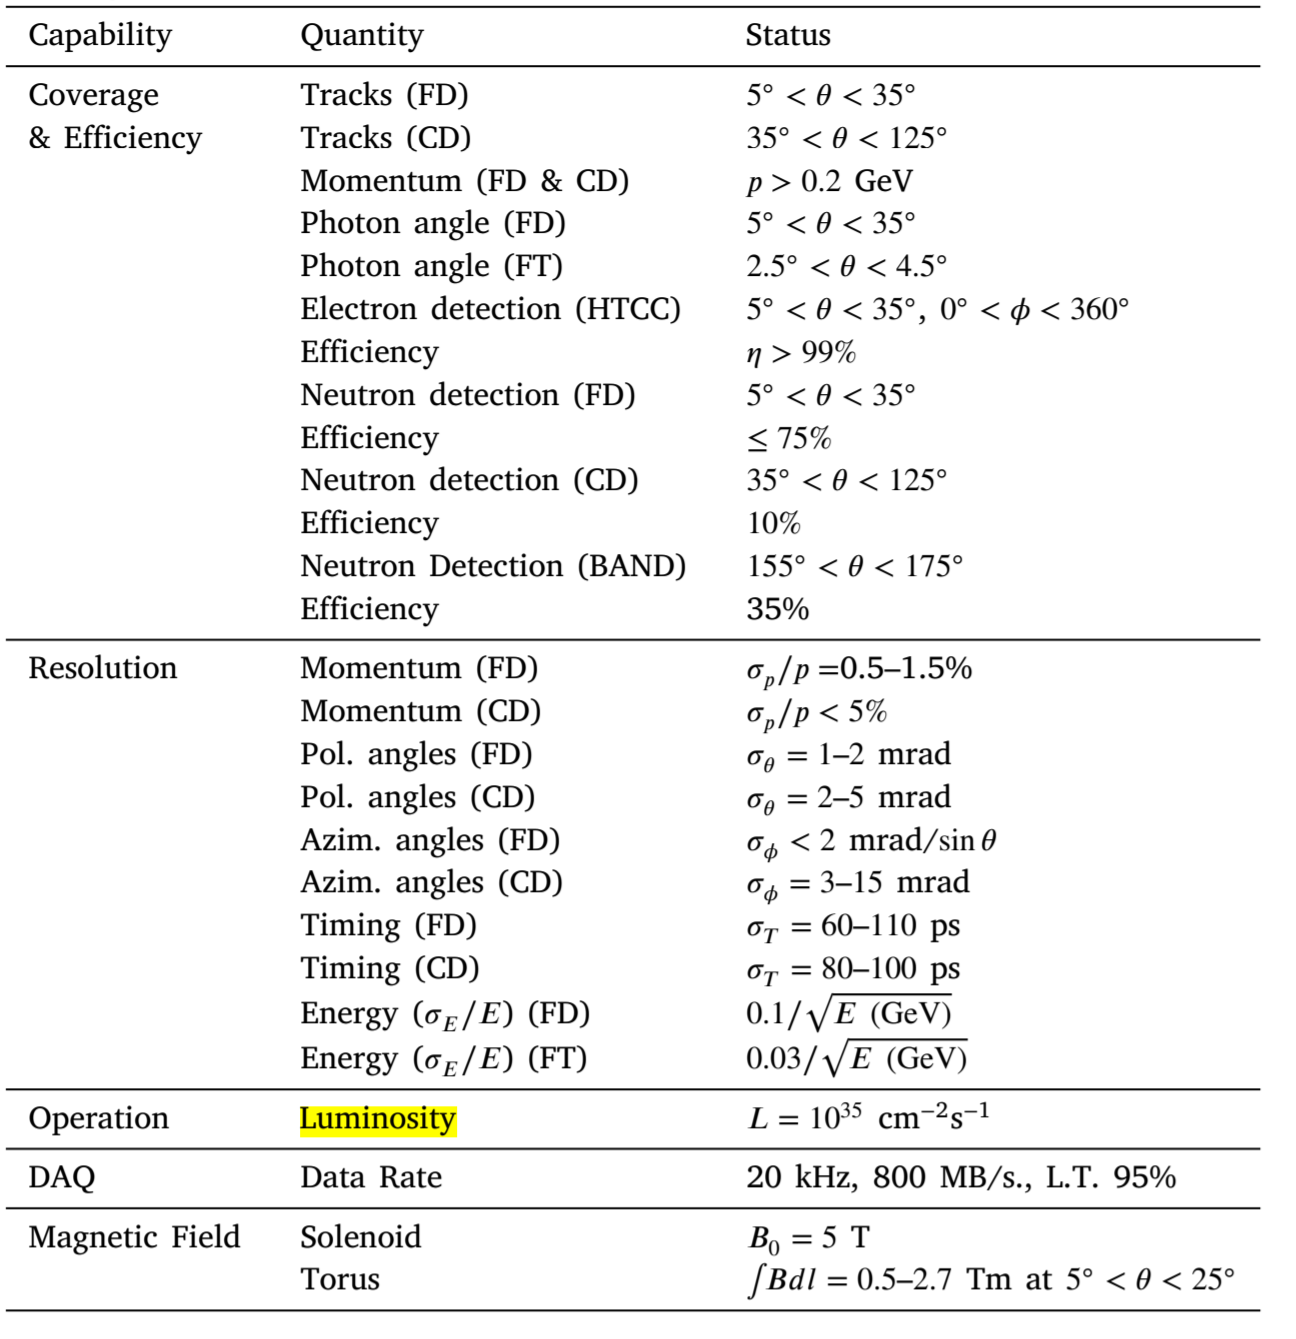
\includegraphics[width=0.3\textwidth]{Chapters/Ch2-Experiment/clas-12-exp/clas-detectors/other/pics/specs-v2-clas12.png}
        }
        \caption{Your caption goes here}
        \label{fig:others}
    \end{figure}

    
    %From sangbaek
    The Data Acquisition (DAQ) \parencite{Boyarinov2020TheSystem} dead-time can be corrected by using a gate at the FC that closes when the DAQ procedure is complete \parencite{Baltzell2020ThePerformance}. The total charge regardless of the gate is called the ungated charge, and the charge collected during the gate on is the gated charge. The ratio of the gated charge to the ungated charge is recorded as the DAQ live-time. The complete listing of detector components can be found in Table. 2.1. The CLAS12 detector components relevant to the particle 4-momentum vector reconstruction are grouped by their characteristics in Table. 2.2. The essential properties like threshold and resolutions and the prominent material components are also listed. 



    Table 2.2: The properties of the relevant subdetectors for the DVCS analysis. The
    properties relate mostly to the effective measurement uncertainties listed in each NIM
    article [135, 136, 140, 141, 143, 144, 147, 152].
    
    \begin{table}[ht]
        \centering
        \begin{tabularx}{\textwidth}{XccXX}
        \toprule
        Name & Coverage ($^\circ$) & Nominal Property & Material \\
        \midrule
        HTCC & 5-35 & $0.015 < p < 4.9$ GeV/c & CO$_2$ \\
        FTOF 1B & 5-35 & $60 - 110$ ps (t) & \\
        FTOF 1A & 5-35 & $90 - 180$ ps (t) & Plastic \\
        FTOF 2 & 35-45 & $170 - 180$ ps (t) & Scintillator \\
        CTOF & 35-125 & $80$ ps (t) & \\
        ECAL & 5-35 & $10\%/\sqrt{E}$ (E) & Pb (absorber) \\
        & & $1.2$ mrad ($\theta, \phi$) & Plastic scintillator \\
        FT-Cal & 2.5-4.5 & $2\%/\sqrt{E} \oplus 1\%$ (E) & PbWO$_4$ crystal \\
        & & $1.5\%$ ($\theta$) & \\
        & & $2^\circ$ ($\phi$) & \\
        DC & 5-40 & $1\%$ (p) & Aluminium wire \\
        & & $1$ mrad ($\theta$) & $90\%$ Ar \\
        & & $1$ mrad/sin $\theta$ ($\phi$) & $10\%$ CO$_2$ \\
        CVT & 35-125 & $5\%$ ($p_t$) & SVT: Si \\
        & & $10 - 20$ mrad ($\theta$) & BMT: $90\%$Ar + $10\%$C$_4$H$_{10}$ \\
        & & $5$ mrad ($\phi$) & \\
        FC & - & $0.48\%$ (L) & Pb \\
        \bottomrule
        \end{tabularx}
        \caption{Caption}
        \label{tab:my_label}
    \end{table}


\fi


    
\subsection{Experiment Run Conditions}
    
The 499 MHz beam structure equates to a signal with a period of 2.004 ns. In practice, the beam was delivered in every other RF bucket, and so bunched at a period of 4.008 ns.

       
            CLAS12 runs with "open trigger", which means different sub-experiments can define their own triggering logic. There is a standard electron trigger, based off of hits in HTCC, ECal, and FTOF. 

        Only about 50\% of the electron triggers recorded with an inbending torus polarity are actually electrons. For outbending torus polarity, hte electron trigger purity is as high at 70\%. 
    
    \href{https://www.jlab.org/Hall-B/clas12-web/}{Detector Specs}
    
    20 kHz Level 1 trigger rate, 1 GB/s.

   The CLAS12 detector is a large angle spectrometer that generally covers angles from 5 to 130 degrees, spanned by two main detector subsystems - the Forward Detector and the Central Detector.

    
   CLAS12 at the design luminosity of 1035 cm−2 s−1

        Data taken is RGA taken in Fall 2018

        Mention configurations and combinatorics


%from sangbaek
In fall 2018, two sets of experiments have been performed with opposite toroidal magnetic field directions
keeping the other detector settings the same. The toroidal magnet bends the scattered
trigger electron inward or outward along the beam direction. In convention, the torus
polarity associated with the inwardly bending electrons is called the negative, -1,
-100\%, or inbending polarity. The opposite is called the positive, +1, +100\%, or
outbending polarity. Both experiments took data with the beam energy of 10.6 GeV,
and the beam current of about 50 nA. The effects due to the variation in the beam
current during the run periods will be taken into account at the end of the analysis.
The CLAS collaboration performed other CLAS12 experiments with different targets
like liquid deuterium, and various beam energies. The description in this thesis
will be focused on the RG-A fall 2018.

The measured
electron beam polarization was 86.9\% during the RG-A data taking in fall 2018.



\section{Reconstruction and Particle Identification}
    here we talk about CLAS PID
\subsection{Decoding and Track Reconstruction}\label{sec:decrec}

\subsection{Particle Identification}


For this analysis all final state particles should be detected.
After $\pi^0$ decay we are going to have 4 particles: electron, proton and two photons.
The particle identification methods are applied to select the exclusive event with at least one electron, proton and two photons. 


    \subsubsection{Electron}
    \subsubsection{Proton}
    \subsubsection{Photon}
    \subsubsection{Pion}
    
    Basic event builder cuts are utilized, then additional cuts are made that are common with the RGA Analysis note (\href{https://www.overleaf.com/project/5ea737720942930001ff5e9c}{overleaf link} and developed by Sangbaek Lee (sangbaek@mit.edu - \href{https://github.com/Sangbaek/analysis_code/tree/analysis/pid}{github code here}. For this analysis, both the central detector and forward detector are utilized for proton tracking. The forward tagger is also utilized for photon identification. 
    


\subsubsection{Neutral pion}
    In addition to individual particle PID procedures the cut on the mass of two photons is applied:
    \begin{itemize}
    	\item $0.07<M_{\gamma\gamma}<0.2$ GeV
    \end{itemize}
    The pion is more thoroughly constrained by the exclusivity cuts, described in the next section.
    

\begin{figure}[hbt]
	\centering
	\includegraphics[page=6,width=0.6\textwidth]{Chapters/Ch4-BaseAnalysis/pid_figs/eppi0.exclusive.pdf}
	
	\caption{The distribution for mass of two photons $M_{\gamma\gamma}$}.
	\label{fig:ggmass}
	
	\centering
	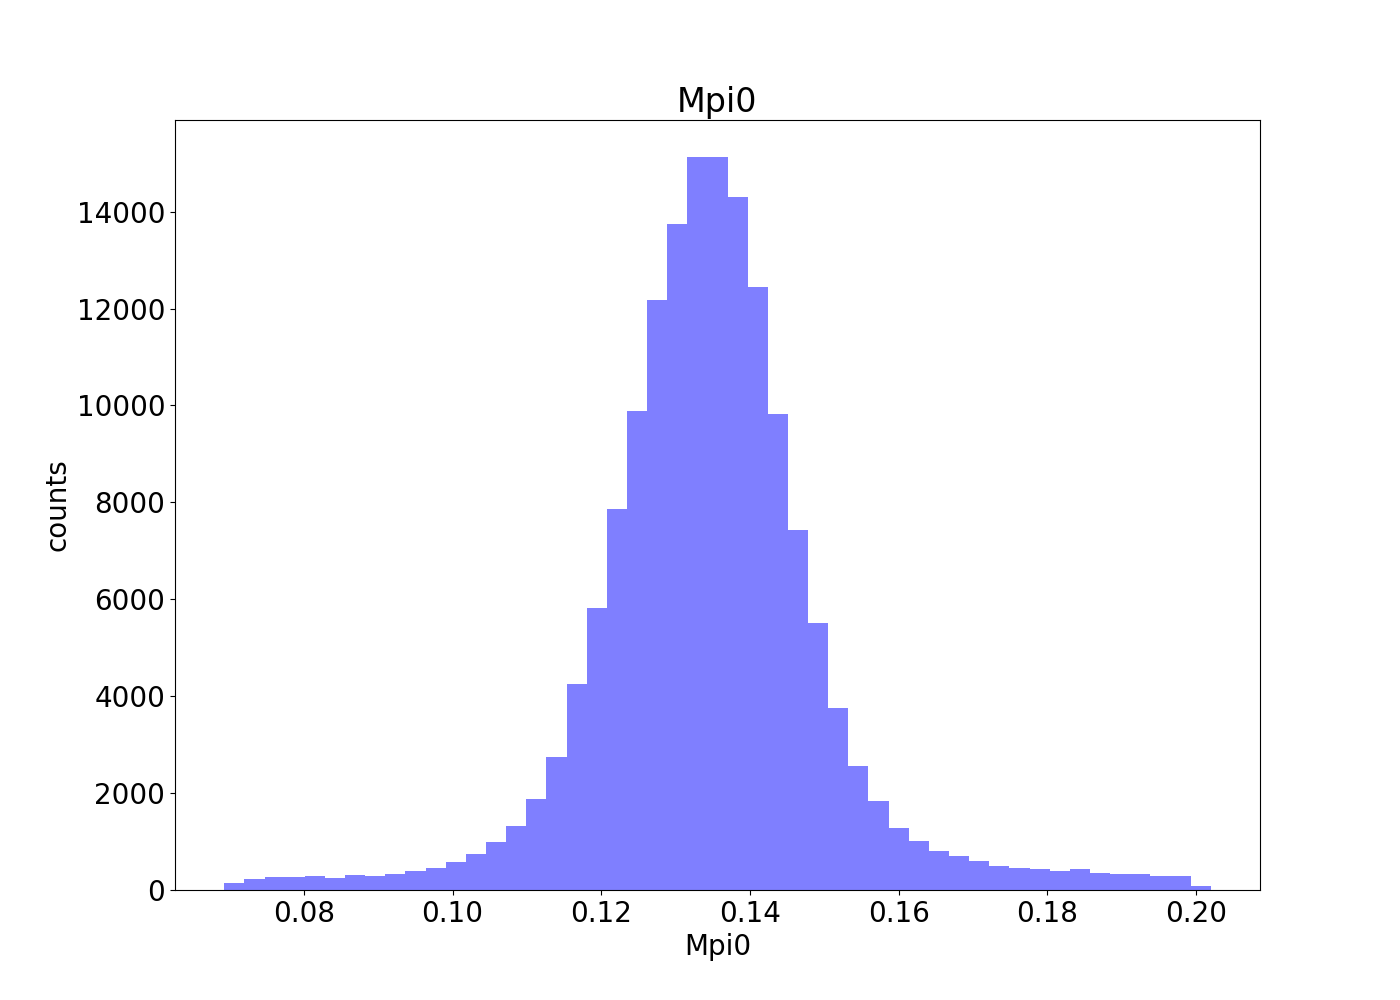
\includegraphics[width=0.6\textwidth]{Chapters/Ch2-Experiment/recon_pid/pid_figs/Mpi0.png}
	
	\caption{The distribution for mass of two photons after exclusivity cuts}.
	\label{fig:ggmass_after}
	
\end{figure}




\subsection{Data Storage and Formatting}
    \subsubsection{Data Location and Availability}
    \subsubsection{File Formatting and Conversion}\label{sec:filtering}
        Mention that same transformations are used for rec events and filtering
    

    








\chapter{Simulations} \label{Chapter:Simulations}
    \section{Simulation Infrastructure}
    \subsection{Motivation for massive simulations}
    \subsection{OSG, MIT Tier 2, submission pipeline}

\section{Generator Details}
    \subsection{AAO}
        \subsection{AAONORAD}
        \subsection{AAORAD}

\section{Simulation Pipeline}
    


\chapter{Data Analysis} \label{Chapter:BaseAnalysis}
    

Official Repo: https://github.com/robertej19/clas12DVPiP
         


For each kinematic bin the differential cross section can be written as:

\begin{equation}
    \sigma = \frac{N_{meas}}{L \epsilon}\frac{1}{\delta}
\end{equation}

Where $\frac{N_{meas}}{L}$ is the number of events from experiment normalized by the integrated luminosity before acceptance and radiatvie corrections. $\epsilon$ = $\frac{N^{RAD}_{rec}}{{N^{RAD}_{gen}}}$ is the acceptance correction and $\delta$ is the radiative correction.



$\delta$ can be obtained by using the following:

\begin{equation}
    \delta = \frac{N^{RAD}_{gen}}{N^{NORAD}_{gen}}
\end{equation}

$\delta$ and $\epsilon$ need to be properly calculated, but for a first pass we will ignore them so we have just



\section{General Analysis Overview}
    \subsection{Part 1}
\Xsecs are theoretically interpreted as  the probability for a specific interaction to occur. They can be experimentally estimated by measuring the occurrence frequency relative to the total possible interaction opportunities. In general, the \xsec $\sigma$ can be expressed as \eqref{eq:basic_xsec} the number of measured events of interest $N_{meas}$ divided by the number of total interaction opportunities \Lumi. \Lumi is known as luminosity and is a product of only experimental parameters, such as the number of particles present and the experiment duration. 

\subsection{part 2}


\begin{equation} \label{eq:basic_xsec}
    \sigma = \frac{\counts}{\Lumi}
\end{equation}

Measuring the complete \xsec at once is not feasible, so instead estimates are made of the differential \xsec \eqref{eq:basic_diff_xsec}, which instead evaluates the probability for a specific interaction to occur in a differential region of phase space, $\frac{d\sigma}{d\Omega}$. Infinitesimal measurements are not possible, so events are counted over some small discretized generalized volume \textcolor{purple}{$\Delta \Omega$}. 

\begin{equation} \label{eq:basic_diff_xsec}
    \frac{d\sigma}{d\Omega} = \frac{ \counts} {\Lumi \textcolor{purple}{\Delta \Omega}}
\end{equation}

In practice, a number of correction terms need to be included to account for differences between experiment and theory. These correction terms, combined with the specifics of this analysis, yield the full experimental expression of the \xsec \eqref{eq:DVPiPCrossSection_exp}. 

     \begin{equation}\labelAndRemember{eq:DVPiPCrossSection_exp}
           { \frac{    d^4\sigma_{  ep \rightarrow ep'\pi^0}   } {dQ^2dx_Bdtd\phi_{\pi}} 
                =   \frac{ \textcolor{red}{ N(Q^2,x_B,t,\phi_{\pi})}} {\Lumiint \textcolor{purple}{ \Delta Q^2 \Delta x_B \Delta t \Delta \phi_{\pi}}} 
                \frac{1}{\textcolor{correctionfactors}{\epsilon_{acc} \delta_{RC} \delta_{Norm} Br(\pi^0\rightarrow\gamma\gamma)}}}
     \end{equation}      \myequations{DV$\pi$P Experimental Cross Section}

The terms on the right-hand side of this equation are: 
\begin{itemize}
\item \textcolor{red}{$N(Q^2,x_B,t,\phi_{\pi})$} - Number of events recorded in a given $Q^2$, $x_B$, $t$, $\phi_{\pi}$ bin.

\item \Lumiint - Integrated luminosity

\item \textcolor{purple}{$\Delta Q^2 \Delta x_B \Delta t \Delta \phi_{\pi}$} - These are the bin sizes or intervals for the variables $Q^2$, $x_B$, $t$, and $\phi_{\pi}$.

\item \textcolor{correctionfactors}{$\epsilon_{acc}$} - Acceptance correction, which is a combination of detector efficiency and geometrical acceptance, determined through simulations. 

\item \textcolor{correctionfactors}{$\delta_{RC}$} - Radiative correction factor

\item \textcolor{correctionfactors}{$\delta_{Norm}$} - Overall normalization factor

\item \textcolor{correctionfactors}{$Br(\pi^0\rightarrow\gamma\gamma)$} - Branching ratio of the decay of a neutral pion ($\pi^0$) into two photons ($\gamma\gamma$), which is most recently measured at 98.8131\%  \cite{Husek2019PreciseDecay}
\end{itemize}


\clearpage
\begin{figure}[!h]
    \centering
    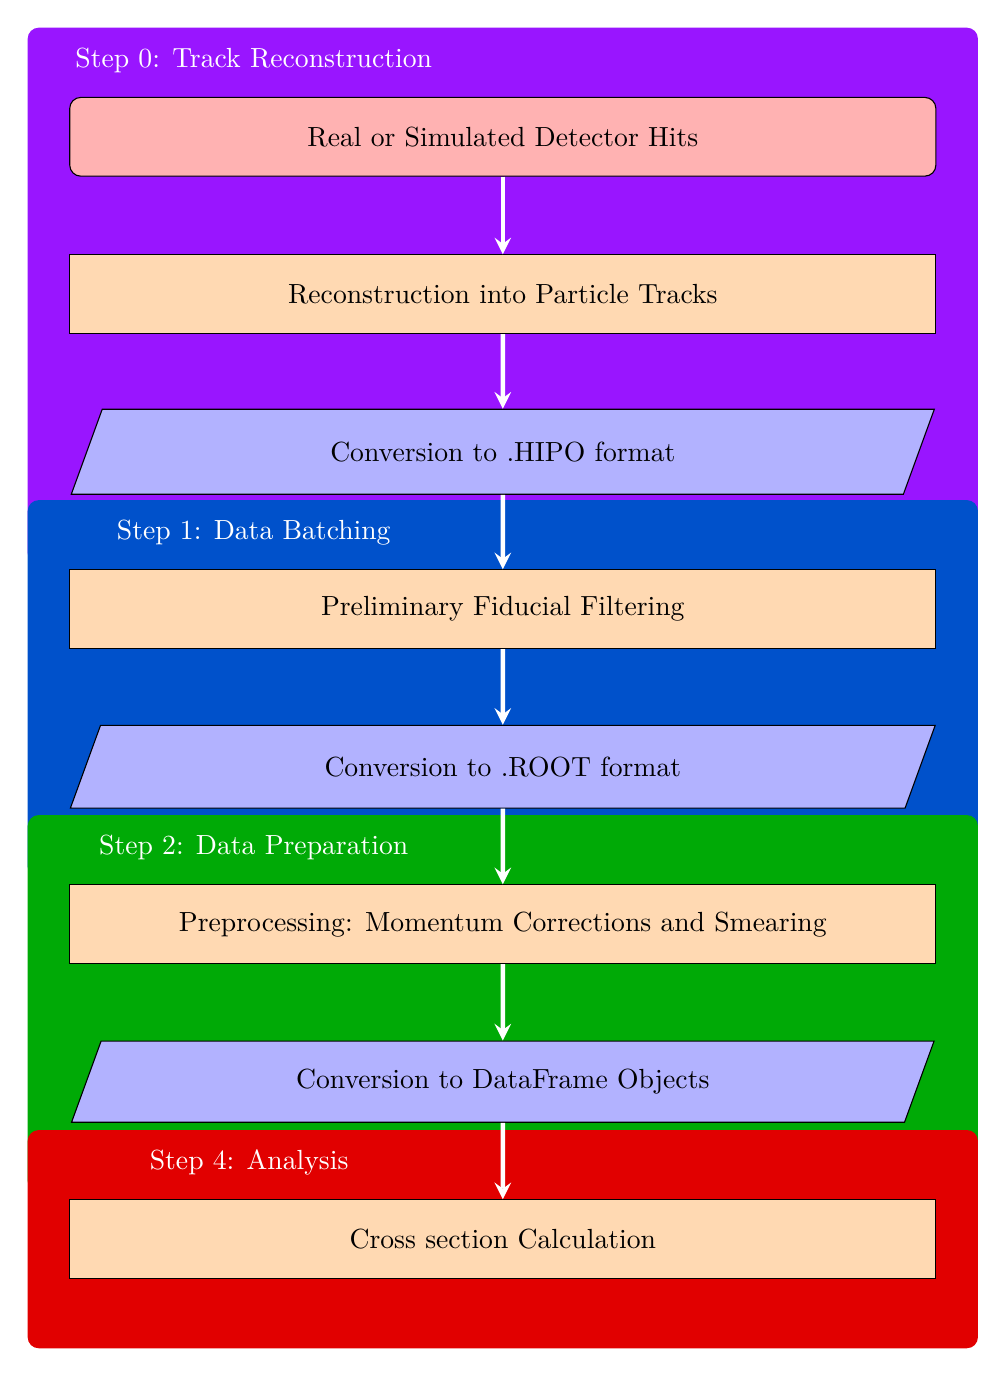
\begin{tikzpicture}[
      node distance=2cm,
      startstop/.style={rectangle, rounded corners, minimum width=11cm, minimum height=1cm,text centered, draw=black, fill=red!30},
      io/.style={trapezium, trapezium left angle=70, trapezium right angle=110, minimum width=11cm, minimum height=1cm, text centered, draw=black, fill=blue!30},
      process/.style={rectangle, minimum width=11cm, minimum height=1cm, text centered, draw=black, fill=orange!30},
      arrow/.style={white,ultra thick,->,>=stealth},
      ]
    
      \node (start) [startstop] {Real or Simulated Detector Hits};
      \node (process1) [process, below of=start] {Reconstruction into Particle Tracks};
      \node (io1) [io, below of=process1] {Conversion to .HIPO format};
      \node (process2) [process, below of=io1] {Preliminary Fiducial Filtering};
      \node (io2) [io, below of=process2] {Conversion to .ROOT format};
      \node (process3) [process, below of=io2] {Preprocessing: Momentum Corrections and Smearing};
      \node (io3) [io, below of=process3] {Conversion to DataFrame Objects};
      \node (process4) [process, below of=io3] {\Xsec Calculation};
       
      \draw [arrow] (start) -- (process1);
      \draw [arrow] (process1) -- (io1);
      \draw [arrow] (io1) -- (process2);
      \draw [arrow] (process2) -- (io2);
      \draw [arrow] (io2) -- (process3);
      \draw [arrow] (process3) -- (io3);
      \draw [arrow] (io3) -- (process4);

    
      \begin{scope}[on background layer]
        \node[fit=(start)(process1)(io1), fill=mypurp, rounded corners, inner xsep=15pt, inner ysep=25pt, label={[xshift=-90pt, yshift=-20pt] north: \textcolor{white}{Step 0: Track Reconstruction} }] {};


        \node[fit=(process2)(io2), fill=darkblue, rounded corners, inner xsep=15pt, inner ysep=25pt, label={[xshift=-90pt, yshift=-20pt] north: \textcolor{white}{Step 1: Data Batching} }] {};


        \node[fit=(process3)(io3), fill=darkgreen, rounded corners, inner xsep=15pt, inner ysep=25pt, label={[xshift=-90pt, yshift=-20pt] north: \textcolor{white}{Step 2: Data Preparation} }] {};

        \node[fit=(process4), fill=darkred, rounded corners, inner xsep=15pt, inner ysep=25pt, label={[xshift=-90pt, yshift=-20pt] north: \textcolor{white}{Step 4: Analysis } }] {};

      \end{scope}
      
    \end{tikzpicture}
    \caption{High-level data processing flow}
    \label{fig:High-level data processing flow}
\end{figure}
    
\section{Data Pre-Processing}
    
In a perfect world, experimental and simulated data could be immediately utilized to compute cross-sections once obtained. In reality, a variety of factors - such as defects in experimental detectors or issues in modeling real-world physics - necessitate minor adjustments to be made to the datasets. It is of course not feasible to re-run entire experiments just to address these small issues, and instead is best handled by pre-processing the data with well-motivated correcting factors.  In particular, the experimental data requires fiducial cuts corresponding to detector dead-zones or otherwise problematic areas, as well as energy loss corrections due to underestimates in the reconstruction scheme. The simulated datasets require smearing factors to more closely resemble the real-world detector and reconstruction algorithm performances.


\subsection{Experimental Data Pre-Processing}\label{sec:momcorr}
     %\subsubsection{Momentum Corrections}{Mom Corr}
%\subsubsection{Energy Loss Corrections}
Charged particles lose energy via ionization and radiation along their paths. Reconstruction schemes attempt to correct for this, but issues can remain in various situations. The electron reconstruction showed negligible deviations from expected performance. The proton reconstruction exhibited a two-band structure due to detector topology, as shown in \ref{fig:protoncorra}. The issue was deeply studied by S. Lee, who developed and implemented a correction scheme \parencite{Lee2022MeasurementDetector}. We demonstrate in \ref{fig:protoncorrb} the correction is functioning as expected in this work. 


    \begin{figure}[H]
        \centering
        
        \subfloat[Distribution without correction. \label{fig:protoncorra}]{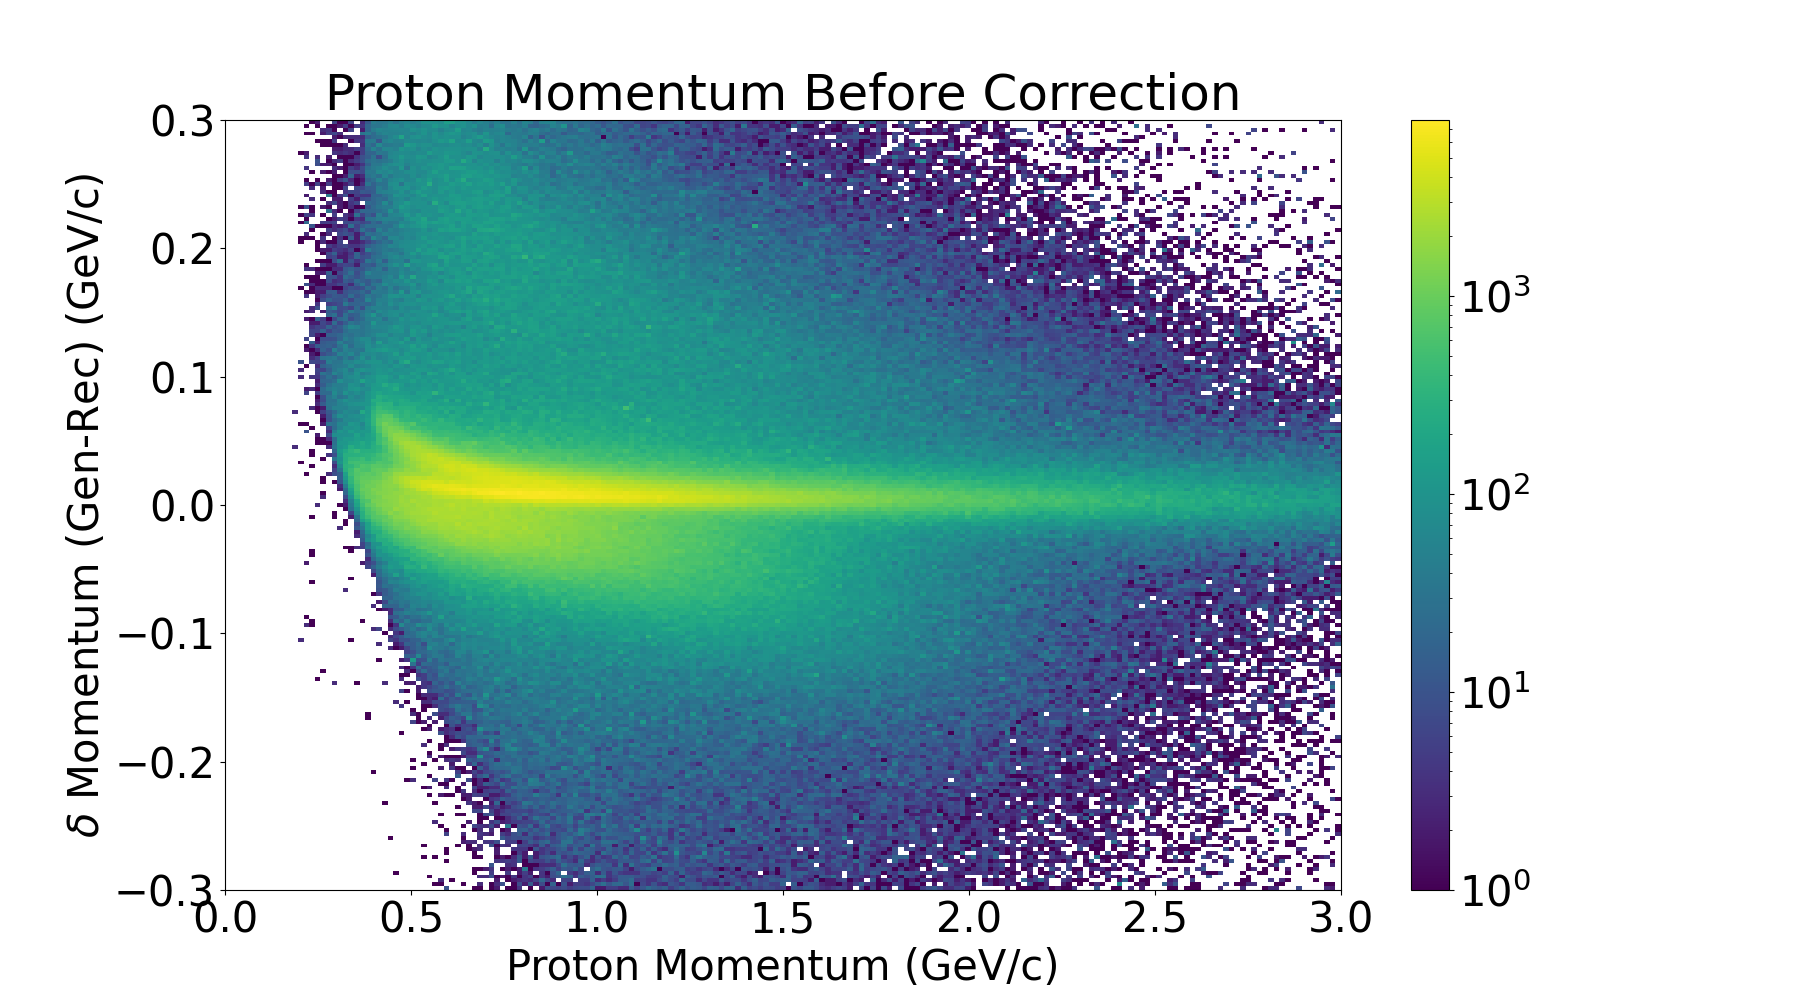
\includegraphics[trim={0 0 5cm 0},clip,width=0.5\textwidth]{Chapters/Ch4-BaseAnalysis/0_preprocessing/0_A_experimental_data_preprocessing/pics/noneProton_Momentum_Before_Correction.png}}
        \hfill
        \subfloat[Distribution with correction. \label{fig:protoncorrb}]{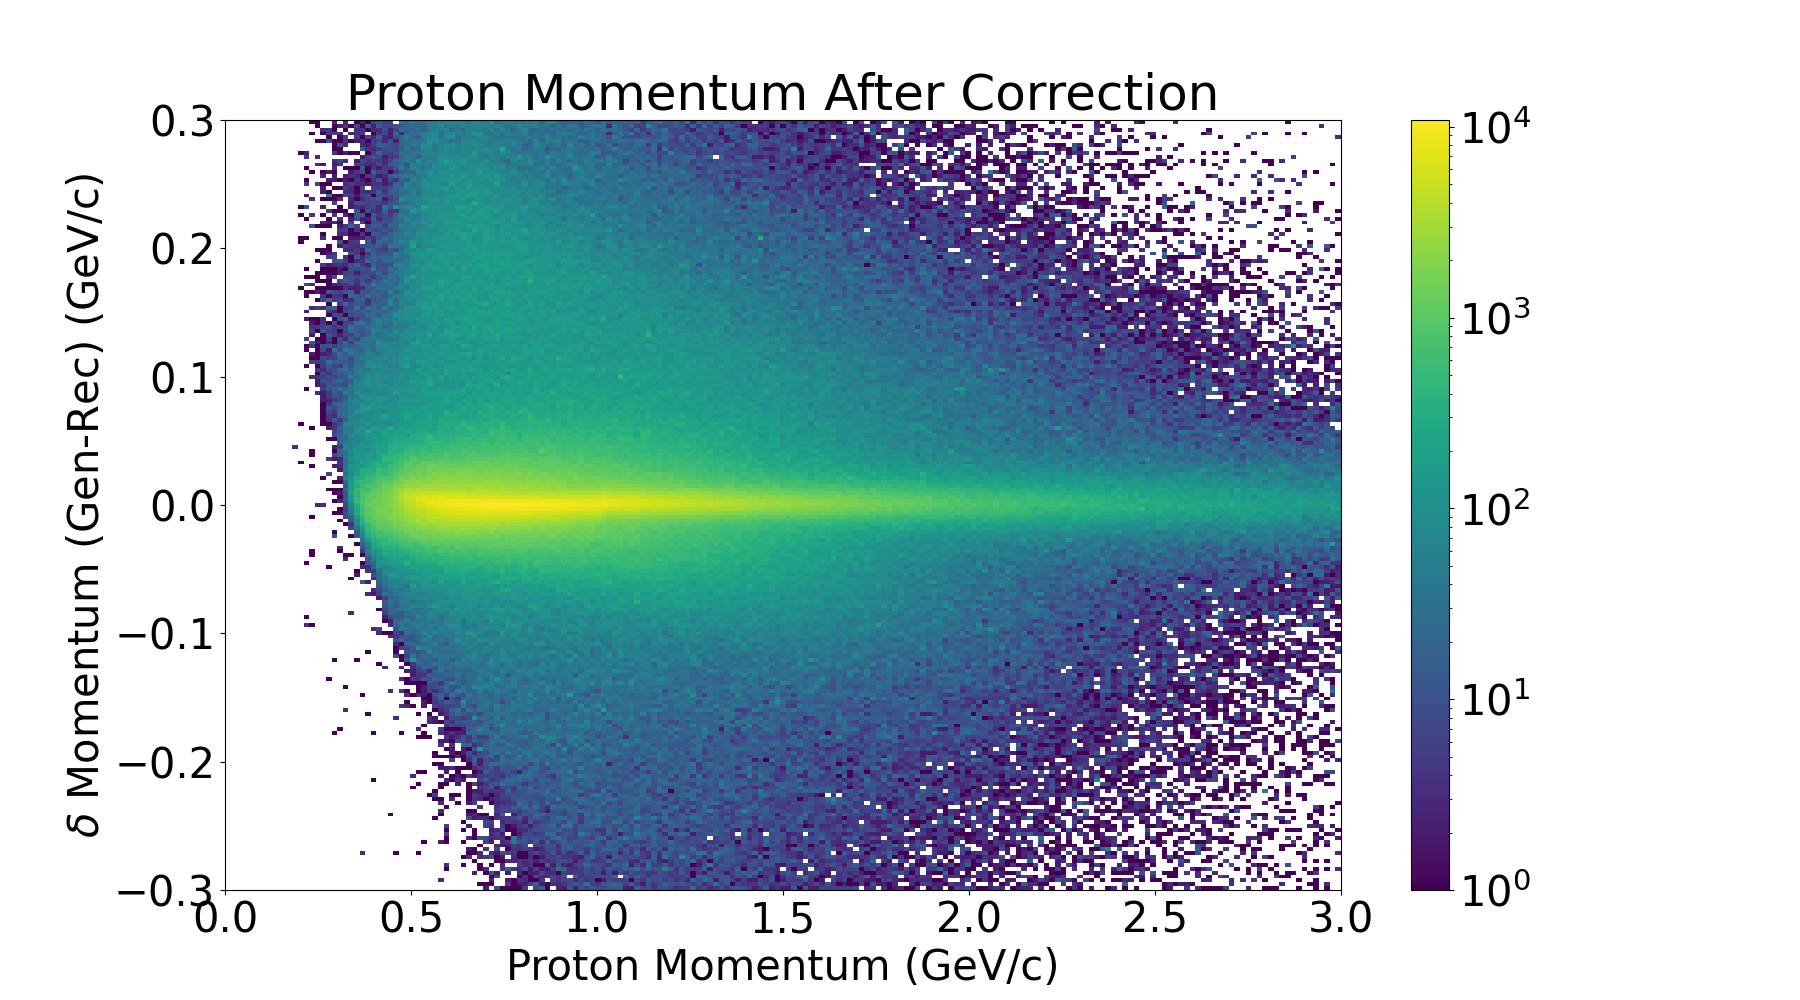
\includegraphics[trim={0 0 5cm 0},clip,width=0.5\textwidth]{Chapters/Ch4-BaseAnalysis/0_preprocessing/0_A_experimental_data_preprocessing/pics/noneProton_Momentum_After_Correction.png}}
    
        \caption[Proton Momentum Correction]{Difference between generated and reconstructed proton momentum as a function of proton momentum, before (a) and after (b) momentum corrections are implemented.}\label{fig:protoncorr}
    \end{figure}

\iffalse
A charged particle loses its energy through its passage through material via ionization
and radiation

We first corrected the energy loss of the proton using the simulation data. After
applying the proton loss corrections to the experimental data and the simulation, we
reduced the reconstruction bias by correcting the single particle kinematics in the
experimental data. To match the resolution, the kinematics of the simulated data
was smeared.

\fi
     
\subsection{Simulation Data Pre-Processing}\label{sec:momsmear}
   %\subsubsection{Simulation:Experiment Resolution Matching}

The detector responses in the GEMC system were modeled to perform slightly better than their real-world counterparts. This means the signal data from the simulations is cleaner than the real experiment, and so smearing factors must be added to provide a better match. This convention was chosen because the alternative (with simulations performing worse than real-world detectors) would yield data that is difficult to deconvolve. \figref{fig:bad} shows the discrepancy between the experimental and simulated data sets, for various variable combinations. 

\begin{figure}[hbt]
	\centering
	\includegraphics[page=125,width=0.3\linewidth]{Chapters/Ch4-BaseAnalysis/0_preprocessing/0_B_simulation_data_preprocessing/pics/nosmear/outbending_rad_All_All_All_no_smearingME_epgg_exp_vs_sim.png}
	\includegraphics[page=123,width=0.3\linewidth]{Chapters/Ch4-BaseAnalysis/0_preprocessing/0_B_simulation_data_preprocessing/pics/nosmear/outbending_rad_All_All_All_no_smearingMM2_egg_exp_vs_sim.png}
	\includegraphics[page=128,width=0.3\linewidth]{Chapters/Ch4-BaseAnalysis/0_preprocessing/0_B_simulation_data_preprocessing/pics/nosmear/outbending_rad_All_All_All_no_smearingMM2_epgg_exp_vs_sim.png}
	\includegraphics[page=130,width=0.3\linewidth]{Chapters/Ch4-BaseAnalysis/0_preprocessing/0_B_simulation_data_preprocessing/pics/nosmear/outbending_rad_All_All_All_no_smearingMM2_ep_exp_vs_sim.png}
	\includegraphics[page=133,width=0.3\linewidth]{Chapters/Ch4-BaseAnalysis/0_preprocessing/0_B_simulation_data_preprocessing/pics/nosmear/outbending_rad_All_All_All_no_smearingMpi0_exp_vs_sim.png}
	\includegraphics[page=135,width=0.3\linewidth]{Chapters/Ch4-BaseAnalysis/0_preprocessing/0_B_simulation_data_preprocessing/pics/nosmear/outbending_rad_All_All_All_no_smearingMPt_exp_vs_sim.png}
	
	\caption[Simulation and Experiment Matching before Smearing]{Comparison of experiment (blue) and simulation (red) missing mass, energy, momentum, and invariant gamma-gamma mass distributions, before any smearing factors were added to the simulation data.}
	\label{fig:bad}
\end{figure}


To improve the matching between simulation and experiment, Gaussian smearing factors were added after reconstruction to the simulated dataset. These factors were tuned by S. Lee \parencite{Lee2022MeasurementDetector} to have optimal matching across all missing mass spectra combinations \figref{fig:good}. In particular, the outgoing proton and photon momenta were smeared with Gaussian kernels with standard deviations $\sigma$ determined as function of momenta and dependent on particle location (CD, FD, or FT).

\begin{figure}[hbt]
	\centering
	\includegraphics[page=125,width=0.3\linewidth]{Chapters/Ch4-BaseAnalysis/0_preprocessing/0_B_simulation_data_preprocessing/pics/yessmear/outbending_rad_All_All_All_for_aps_2022_plots_sangcutsME_epgg_exp_vs_sim.png}
	\includegraphics[page=123,width=0.3\linewidth]{Chapters/Ch4-BaseAnalysis/0_preprocessing/0_B_simulation_data_preprocessing/pics/yessmear/outbending_rad_All_All_All_for_aps_2022_plots_sangcutsMM2_egg_exp_vs_sim.png}
	\includegraphics[page=128,width=0.3\linewidth]{Chapters/Ch4-BaseAnalysis/0_preprocessing/0_B_simulation_data_preprocessing/pics/yessmear/outbending_rad_All_All_All_for_aps_2022_plots_sangcutsMM2_epgg_exp_vs_sim.png}
	\includegraphics[page=130,width=0.3\linewidth]{Chapters/Ch4-BaseAnalysis/0_preprocessing/0_B_simulation_data_preprocessing/pics/yessmear/outbending_rad_All_All_All_for_aps_2022_plots_sangcutsMM2_ep_exp_vs_sim.png}
	\includegraphics[page=133,width=0.3\linewidth]{Chapters/Ch4-BaseAnalysis/0_preprocessing/0_B_simulation_data_preprocessing/pics/yessmear/outbending_rad_All_All_All_for_aps_2022_plots_sangcutsMpi0_exp_vs_sim.png}
	\includegraphics[page=135,width=0.3\linewidth]{Chapters/Ch4-BaseAnalysis/0_preprocessing/0_B_simulation_data_preprocessing/pics/yessmear/outbending_rad_All_All_All_for_aps_2022_plots_sangcutsMPt_exp_vs_sim.png}
	
	\caption[Simulation and Experiment Matching after Smearing]{Comparison of experiment (blue) and simulation (red) missing mass, energy, momentum, and invariant gamma-gamma mass distributions, with smearing factors added to the simulation data proton and photon momenta.}
	\label{fig:good}
\end{figure}






\section{Event Selection}
    Overview words about event selection

\subsection{Exclusivity Cuts}\label{sec:eventselection}

    \begin{wrapfigure}{r}{0.58\textwidth}
    	\vspace*{-0.3cm}
    	\includegraphics[page=10,width=0.97\linewidth]{Chapters/Ch4-BaseAnalysis/1_Event_Selection_Cuts/figures/eppi0.exclusive.pdf}
    	\caption{MM$^2$ (epX) vs $\theta_X\pi$ 2D distribution.}
    	\label{fig:MM2vsThetaXPi}
    \end{wrapfigure}
    After the selection of events with at least one electron, proton and two photons, it is time to take a look at the exclusive distributions.
    The Fig.~\ref{fig:MM2vsThetaXPi} shows 2D distribution of MM$^2$ (epX) vs $\theta_{X\pi}$, where MM$^2$ (epX) is a missing mass squared of (epX) system and should have a peak near 0.0182 GeV$^2$, and $\theta_{X\pi}$ is an angle between expected and reconstructed pion.
    The bright spot on the figure corresponds to the exclusive $ep\rightarrow~ep\pi^0$ events.
    In order to reduce the background exclusivity cuts  need to be developed based on the conservation of energy and momentum.
    The relevant 1D exclusive distributions are shown on the Fig.~\ref{fig:rawexclusive1} and \ref{fig:rawexclusive2}.
    
    \begin{figure}[hbt]
    	\centering
    	\includegraphics[page=4,width=0.47\linewidth]{Chapters/Ch4-BaseAnalysis/1_Event_Selection_Cuts/figures/eppi0.exclusive.pdf}
    	\includegraphics[page=5,width=0.47\linewidth]{Chapters/Ch4-BaseAnalysis/1_Event_Selection_Cuts/figures/eppi0.exclusive.pdf}
    	\caption{Exclusive distributions for events with at least one electron, proton and two photons.}
    	\label{fig:rawexclusive1}
    \end{figure}
    
    \begin{figure}[hbt]
    	\centering
    	\includegraphics[page=6,width=0.47\linewidth]{Chapters/Ch4-BaseAnalysis/1_Event_Selection_Cuts/figures/eppi0.exclusive.pdf}
    	\includegraphics[page=8,width=0.47\linewidth]{Chapters/Ch4-BaseAnalysis/1_Event_Selection_Cuts/figures/eppi0.exclusive.pdf}
    	\caption{Exclusive distributions for events with at least one electron, proton and two photons.}
    	\label{fig:rawexclusive2}
    \end{figure}
    
    \subsubsection{Tight \texorpdfstring{$M_{\gamma\gamma} $} mass and transverse missing momenta cuts}
    
    The first step is to use tighter $\gamma\gamma$ mass cut: $0.096<M_{\gamma\gamma}<0.168$ GeV, and take a look at the missing transverse momentum distributions (see Fig.~\ref{fig:ptdistributions}).
    From momentum conservation law we expect transverse momentum to be zero, so we can apply cuts on $\Delta p_x$ and $\Delta p_y$ to further improve exclusive channel selection.
    The cuts $|\Delta p_x|<0.2$ and $|\Delta p_y|<0.2$ correspond roughly to 4-5 $\sigma$.
    
    \begin{figure}[hbt]
    	\centering
    	\includegraphics[page=24,width=0.47\linewidth]{Chapters/Ch4-BaseAnalysis/1_Event_Selection_Cuts/figures/eppi0.exclusive.pdf}
    	\includegraphics[page=25,width=0.47\linewidth]{Chapters/Ch4-BaseAnalysis/1_Event_Selection_Cuts/figures/eppi0.exclusive.pdf}
    	\caption{Exclusive distributions for events with at least one electron, proton and two photons.}
    	\label{fig:ptdistributions}
    \end{figure}
    
    The exclusive distributions after tight $M_{\gamma\gamma}$ mass and transverse missing momenta cuts are shown on Fig.~\ref{fig:rawexclusive3} and display much stronger signal peaks on top of reduced background.
    
    \begin{figure}[hbt]
    	\centering
    	\includegraphics[page=43,width=0.45\linewidth]{Chapters/Ch4-BaseAnalysis/1_Event_Selection_Cuts/figures/eppi0.exclusive.pdf}
    	\includegraphics[page=44,width=0.45\linewidth]{Chapters/Ch4-BaseAnalysis/1_Event_Selection_Cuts/figures/eppi0.exclusive.pdf}
    	\includegraphics[page=45,width=0.45\linewidth]{Chapters/Ch4-BaseAnalysis/1_Event_Selection_Cuts/figures/eppi0.exclusive.pdf}
        \includegraphics[page=47,width=0.45\linewidth]{Chapters/Ch4-BaseAnalysis/1_Event_Selection_Cuts/figures/eppi0.exclusive.pdf}
    
    	\caption{Exclusive distributions after tight $M_{\gamma\gamma}$ mass and transverse missing momenta cuts .}
    	\label{fig:rawexclusive3}
    \end{figure}
    
    \subsubsection{\texorpdfstring{$\theta_{X\pi}$} cut determination}
    
    The cut on angle between expected and reconstructed pion is used in order to further reduce background.
    To choose the value of the $\theta_{X\pi}$ cut the $MM^2(epX)$ distribution is analyzed at multiple $\theta_{X\pi}$ cut values and fit using gaussian+polynomial function as shown on Fig.~\ref{fig:mm2fordifferenttheta}.
    From the fit we can estimate the number of good exclusive events (gaussian) and the number of background events (polynomial) and their dependence on $\theta_{X\pi}$ cut.
    Fig.~\ref{fig:sigbgvsthetacutQ2} and~\ref{fig:sigbgvsthetacutxB} show the numbers of signal and background events as functions of $\theta_{X\pi}$ cut value for multiple bins in $Q^2$ and $x_B$.
    These plots show that the cut $\theta_{X\pi}<2^\circ$ allows to select the most number of good events with the least background, and relaxing it beyond $2^\circ$ does not gain us any good exclusive events but increases background.
    
    
    \begin{figure}[hbt]
    	\centering
    	\includegraphics[page=123,width=0.3\linewidth]{Chapters/Ch4-BaseAnalysis/1_Event_Selection_Cuts/figures/sigbg_eppi0.pdf}
    	\includegraphics[page=125,width=0.3\linewidth]{Chapters/Ch4-BaseAnalysis/1_Event_Selection_Cuts/figures/sigbg_eppi0.pdf}
    	\includegraphics[page=128,width=0.3\linewidth]{Chapters/Ch4-BaseAnalysis/1_Event_Selection_Cuts/figures/sigbg_eppi0.pdf}
    	\includegraphics[page=130,width=0.3\linewidth]{Chapters/Ch4-BaseAnalysis/1_Event_Selection_Cuts/figures/sigbg_eppi0.pdf}
    	\includegraphics[page=133,width=0.3\linewidth]{Chapters/Ch4-BaseAnalysis/1_Event_Selection_Cuts/figures/sigbg_eppi0.pdf}
    	\includegraphics[page=135,width=0.3\linewidth]{Chapters/Ch4-BaseAnalysis/1_Event_Selection_Cuts/figures/sigbg_eppi0.pdf}
    	
    	\caption{$MM^2(epX)$ distributions for multiple $\theta_{X\pi}$ cut values.}
    	\label{fig:mm2fordifferenttheta}
    \end{figure}
    
    
    \begin{figure}[hbt]
    	\centering
    	
    	\includegraphics[width=0.32\linewidth,page=34]{Chapters/Ch4-BaseAnalysis/1_Event_Selection_Cuts/figures/sigbg_eppi0.pdf}
    	\includegraphics[width=0.32\linewidth,page=51]{Chapters/Ch4-BaseAnalysis/1_Event_Selection_Cuts/figures/sigbg_eppi0.pdf}
    	\includegraphics[width=0.32\linewidth,page=68]{Chapters/Ch4-BaseAnalysis/1_Event_Selection_Cuts/figures/sigbg_eppi0.pdf}
    	\includegraphics[width=0.32\linewidth,page=85]{Chapters/Ch4-BaseAnalysis/1_Event_Selection_Cuts/figures/sigbg_eppi0.pdf}
    	\includegraphics[width=0.32\linewidth,page=102]{Chapters/Ch4-BaseAnalysis/1_Event_Selection_Cuts/figures/sigbg_eppi0.pdf}
    	\includegraphics[width=0.32\linewidth,page=119]{Chapters/Ch4-BaseAnalysis/1_Event_Selection_Cuts/figures/sigbg_eppi0.pdf}
    	
    	\caption{The numbers of signal (red markers) and background (black markers) events as functions of $\theta_{X\pi}$ cut value for multiple $Q^2$ bins.}
    	\label{fig:sigbgvsthetacutQ2}
    \end{figure}
    
    
    \begin{figure}[hbt]
    	\centering
    	
    	\includegraphics[width=0.32\linewidth,page=136]{Chapters/Ch4-BaseAnalysis/1_Event_Selection_Cuts/figures/sigbg_eppi0.pdf}
    	\includegraphics[width=0.32\linewidth,page=153]{Chapters/Ch4-BaseAnalysis/1_Event_Selection_Cuts/figures/sigbg_eppi0.pdf}
    	\includegraphics[width=0.32\linewidth,page=170]{Chapters/Ch4-BaseAnalysis/1_Event_Selection_Cuts/figures/sigbg_eppi0.pdf}
    	\includegraphics[width=0.32\linewidth,page=187]{Chapters/Ch4-BaseAnalysis/1_Event_Selection_Cuts/figures/sigbg_eppi0.pdf}
    	\includegraphics[width=0.32\linewidth,page=204]{Chapters/Ch4-BaseAnalysis/1_Event_Selection_Cuts/figures/sigbg_eppi0.pdf}
    	
    	\caption{The numbers of signal (red markers) and background (black markers) events as functions of $\theta_{X\pi}$ cut value for multiple $x_B$ bins.}
    	\label{fig:sigbgvsthetacutxB}
    \end{figure}
    
    \clearpage
    
    \subsubsection{Final exclusivity cuts}
    
    The list of final exclusive cuts is following:
    \begin{itemize}
    	\item $\Delta p_x<0.2$ GeV
    	\item $\Delta p_y<0.2$ GeV
    	\item $\theta_{X\pi}<2^\circ$
    	\item $0.096<M_{\gamma\gamma}<0.168$ GeV
    	\item $MM^2(epX)<0.5$ GeV$^2$
    \end{itemize}
    
    Exclusive distributions after all exclusivity cut except $MM^2(epX)<0.5$ GeV are shown on Fig.~\ref{fig:finalexclusive}
    
    \begin{figure}[hbt]
    	\centering
    	
    	\includegraphics[page=82,width=0.32\linewidth]{Chapters/Ch4-BaseAnalysis/1_Event_Selection_Cuts/figures/eppi0.exclusive.pdf}
    	\includegraphics[page=83,width=0.32\linewidth]{Chapters/Ch4-BaseAnalysis/1_Event_Selection_Cuts/figures/eppi0.exclusive.pdf}
    	\includegraphics[page=84,width=0.32\linewidth]{Chapters/Ch4-BaseAnalysis/1_Event_Selection_Cuts/figures/eppi0.exclusive.pdf}
    	\caption{Exclusive distributions after all exclusivity cuts .}
    	\label{fig:finalexclusive}
    \end{figure}
    
    
    
    
    
    
    
    To arrive at a DVEP candidate event, we do the following
    
    
    Code flow:
    
    Consider a directory with n hipo files. For each hipo file, do the following.
    
    Read each file event by event, and do the following
    
    Check that the event has the proper databanks, and if not, go to teh next event.
    
    Get a list of all the electrons*, protons*, and photons* in the event
    
    *= links to most up to date PID methods
    
    for every electron in the event (always only one, at least in the skims, but not held to be one) do the following
    For every proton in the event, do the following
    
    Calculate some basic quantities and fill histograms
    
    for every permutation of pairs of photons in the event, do the following
    
    calculate various kinematic quantities, and pass to see if creates a viable pion* and a viable DVEP event*
    
    if so, fill relevant histograms and count as a DVEP event, otherwise skip to next event
    
    viable pion: 
    pion mass betwen 100 and 180 MeV
    pion momentum greater than 1.5 GeV
    angle (theta) between each photon and the electron to be greater than 8 degrees
    
    viable DVEP event:
    Q2 greater than 1
    W greater than 2
    difference between theta of missing 4-momentum and reconstructed pion less than 2 degrees
    difference between missing X px and py 300 MeV each or less
    Difference in missing mass squared between pion and X less than 1 GeV ** make sure this is right
    difference in missing energy and X less than 1 GeV **make sure this is right
    

\iffalse
\subsection{Kinematic Fitting}

    Instead of rigid cuts, we can use maximum likelihood estimators - include notes from Janet's class

    The first issue arises with event classification - although we want to examine events with a neutral pion (which decays
to two photons), a proton, and an electron, in practice we create a huge amount of data that is consistent with either pure
noise, or from other hadronic processes. We must classify each of the many millions of recorded events as either signal or
noise. This is traditionally done over the union of single parameter classifications with rigid boundaries as a box in parameter
space (e.g. a signal event is one which satisfies a strict set of conditions). Unfortunately, this excludes many valid events that
were reconstructed poorly in only one or a few of the many (roughly 20) different parameters under consideration. This firstly
reduces the data sample size, which is relatively expensive to obtain, and secondly introduces large systematic uncertainties
into the analysis. A more advanced approached is to use machine learning classifiers to improve event selection and decrease
signal uncertainty. This more advanced method of classification is currently being implemented and verified in the analysis to
demonstrate that it supplants the traditional method effectively


    \begin{table}[h]
        \centering
        \begin{tabular}{c|ccc}
            \textbf{Configuration} & \textbf{Gen. Type} & \textbf{Background} & \textbf{Nevents (MM)} \\ \hline
                & norad & none & 5 \\
                & norad & 50 nA & 5 \\
            Inbending & rad & 50 nA & 15 \\
                & rad & 45 nA & 10 \\
                & rad & 55 nA & 10 \\ \hline
                & norad & none & 10 \\
                & norad &  50 nA & 10 \\
            Outbending & rad & 50 nA & 30 \\
                 & rad & 40 nA & 10 \\
             & rad & 40 nA (+1.01) & 10 \\
            \hline
            Total & - & - & 1400 \\
        \end{tabular}
    \caption[Distribution of Simulated Events by Configuration]{Number of simulated events for various experimental configurations and conditions.\tabref{table:Generated_Data} shows the corresponding number of generated events per distribution. \textcolor{red}{\textbf{NOTE: Values in this table are placeholders and need to be updated with final figures}}}
    \label{table:simulated_data}
    \end{table}
\fi
    
\section{Luminosity}\label{sec:luminosity}
    
%The strategy to calculate the luminosity is as follows:\\

% - For each run, retrieve a measure of how much beam passed through the target, I believe in the case of CLAS12 using the Faraday cup to measure beam charge
%    - sum the beam charge over all runs being considered and include any relevant corrections factors
%    - multiply this by target length, density, etc. to get the integrated luminosity
%    - use this value to calculate cross sections.

%Compare integrated luminosity of CLAS6 to CLAS12 (in 2011 analysis note)

Luminosity can calculated according to equation \ref{lumieq}
 \begin{equation}\label{lumieq}
            \Lumi = \frac{N_A l \rho Q_{FCUP}}{e}.
\end{equation}

$N_A$ is Avogadro's constant, l is the length of the target,  $\rho$ is the density of the target (liquid hydrogen), $Q_{FCUP}$ is the charge collected on the Faraday cup, and e is the charge of the electron. The values of these quantities are are as tabulated in table \ref{lumitable}. 


\begin{table}[h]
    \centering
    \begin{tabular}{rcc}
         %& Heading 1 & Heading 2 \\\hline
        Quantity & Symbol & CLAS12 Value \\\hline
       Avogadro's Number &  N$_A$  & 6.02214 x $10^{23}$ \\
        Electron Charge &e  &  1.602 x 10$^{-19}$ Coulombs \\
        Target Length &l &  5.00 cm \\
        Target Density &$\rho$  &  0.07 $g/cm^3$ (LH2) \\
        Charge on Faraday Cup & $Q_{FCUP}$ &  In data\\
    \end{tabular}
\caption[Terms of Luminosity Equation]{Values of terms in luminosity determination.}
\end{table}\label{lumitable}

The accumulated charge on the Faraday cup is calculated by taking the difference between the maximum and minimum values of beamQ for each run (events are not necessarily time ordered), and then summing these values. Typical runs at CLAS12 have an accumulated beam charge of tens to hundreds of thousands of nanoCoulombs. 

The Fall 2018 Inbending configuration integrated luminosity was calculated to be \Lumiint = 5.511802 x 10$^{40}$ $cm^{-2}$  = 5.511802 x 10$^{7}$  inverse femtobarns, and the Fall 2018 Outbending configuration was found to have \Lumiint = 4.651647 x 10$^{7}$ $fb^{-1}$



\iffalse
Implementation:
The bank \texttt{REC::Event} has an object \texttt{beamCharge}, in nanoCoulombs, which is described in the \texttt{DST} as ``beam charge integrated from the beginning of the run to the most recent reading of the gated Faraday Cup scaler in \texttt{RAW::scaler}, with slope/offset conversion to charge from CCDB. Note, this value will be zero in each file until the first scaler reading in that file.''. This is the (un?)gated beam charge. 


This can be accessed via:

\begin{lstlisting}
	def banknames = ['REC::Event','REC::Particle','REC::Cherenkov','REC::Calorimeter','REC::Traj','REC::Track','REC::Scintillator']

	if(banknames.every{event.hasBank(it)}) {
		def (evb,partb,cc,ec,traj,trck,scib) = banknames.collect{event.getBank(it)}
def fcupBeamCharge = evb.getFloat('beamCharge',0)
\end{lstlisting}

    According to \href{https://clas12.discourse.group/t/accessing-beam-charge-information/239}{this} we might need to use tag=1 RAW::scaler::fcupgated instead of REC::Event::beamCharge
\fi


\section{Binning}
    To the author's knowledge, there is no singular mathematically optimized binning scheme criterion for a generalized 4-dimensional dataset. Concordantly, the multidimensional binning in this analysis was heuristically informed 


    \begin{figure}[H]
        \centering

        
        \subfloat[Inbending $xB$ vs. $Q^2$]{\includegraphics[trim={0 0 5cm 0},clip,width=0.5\textwidth]{Chapters/Ch4-BaseAnalysis/3_Binning/pics/x_B_vs_Q2,_Exp_Inbend.png}}
        \hfill
        \subfloat[Inbending $\phi$ vs. $t$]{\includegraphics[trim={0 0 5cm 0},clip,width=0.5\textwidth]{Chapters/Ch4-BaseAnalysis/3_Binning/pics/phi_vs_Momentum_Transfer_t,_Exp_Inbend.png}}

        \subfloat[Outbending $xB$ vs. $Q^2$]{\includegraphics[trim={0 0 5cm 0},clip,width=0.5\textwidth]{Chapters/Ch4-BaseAnalysis/3_Binning/pics/x_B_vs_Q2,_Exp_Outbend.png}}
        \hfill
        \subfloat[Outbending $\phi$ vs. $t$]{\includegraphics[trim={0 0 5cm 0},clip,width=0.5\textwidth]{Chapters/Ch4-BaseAnalysis/3_Binning/pics/phi_vs_Momentum_Transfer_t,_Exp_Outbend.png}}

        \caption[CLAS12 Data Binning Scheme]{Binning scheme for CLAS12 Fall 2018 Inbending (top row) and Fall 2018 Outbending (bottom row) datasets.}\label{fig:clas12_sub_portal}
    \end{figure}

Was chosen to overlap previous results \parencite{Bedlinskiy2014ExclusiveCLAS} to facilitate data comparisons. 

From equation 1.12

W2 = Q/x+m - Q = 4 -- Q = (4 - m) / (1/x - 1)

8.604^2 < q2
W >

 Q/x+m - Q >4

Q2< 74.028816





To avoid bin migration, set high q2 on generation.

\iffalse
Figure 5-19: The 2D histograms of events in ��2 and ���� for each configuration of final
level BH-DVCS events. The kinematic regions are bordered by the certain required
conditions: (1) ����′ > 2 GeV/c (green), (2) ��2 > 1 (GeV/c)2 (blue) and (3) �� > 2
GeV (red).

finite bin effects - center is not average  mean diff

bin volume correction - distribution cutoffs

It is important to choose an optimal multidimensional binning scheme for the cross
section extraction. In this thesis, the bin shape was designed to be a four dimensional
box. Some bins are not well fitted into the box due to the phase space condition. For
example, Fig. 5-19 shows several triangular bins in the ��2 −���� plane at the left side,
whose hypotenuse is determined by ����′ > 2 GeV/c.
The advantage of finer binning is to provide improved density estimation. The
acceptance corrections and the finite bin width effects should increase with the bin
size. However, the bin size cannot be narrower than the effective resolutions in the
binning variables to minimize bin migration. Extremely small bins would not have
any statistical significance in each bin, which would lead to an invalid analysis. It is
important to determine the optimal binning.


The different proton momentum thresholds were considered for the |��| binning.
The momentum thresholds required for the proton momentum reconstruction, 0.3
GeV/c for CD, 0.42 GeV/c for FD inbending, 0.5 GeV/c for FD outbending lead to
|��| threhsold of 0.09, 0.17 and 0.23 GeV2 respectively. To consider the bin migration
effect, the |��| bin was loosely set as [0.110, 0.150, 0.250, 0.400, 0.600, 0.800, 1.000]
GeV2. The number of events in the first bin was estimated with CD protons only.
Likewise, the FD outbending data was not used for the second bin event counting.
There are not enough statistics above |t|=1 GeV2 to determine the cross sections with
reasonable precision from the RG-A fall 2018 data alone.

The ��2−���� phase space was evenly divided by the bin edges [1.000, 1.200, 1.456,
1.912, 2.510, 3.295, 4.326, 5.761, 7.000] (GeV/c)2 and [0.062, 0.090, 0.118, 0.155,
0.204, 0.268, 0.357, 0.446, 0.581]. The ��2 − ���� bin boundaries are presented in
��2 − ���� plane with the 2D histogram of entire experimental data set in Fig. 5-19
with an explanation of the kinematics boundaries at the caption


The �� distributions are binned in equal width bins of width 15∘. Other possible
binning schemes include (1) the adjusted equal width binning to widen the bin width
at the central region to compensate for low statistics, and (2) the equal frequency

binning. The chosen binning scheme has three advantages; (1) the binning scheme is
symmetric with respect to �� = 180∘, (2) the frequency is directly translated into the
probability distribution in the same ��2 − ���� − |��| bin, and (3) it was used by other
experiments [107, 129].

\fi

\section{Correction Factors}
    \subsection{Acceptance Correction}
The largest correction factor in this work is the acceptance correction, which is a convolution of detector efficiency, geometrical acceptance, reconstruction efficiency, and PID and event cuts. We defined acceptance in \eqref{eq:acceptance} as

    \begin{equation*}
      \recallLabel{eq:acceptance},
    \end{equation*}

where we utilize simulations to arrive at an estimator for the acceptance, $\hat{\epsilon}$. The correction term is calculated bin-by-bin, procedurally illustrated in \figref{fig:acccorr}. As defined, $\hat{\epsilon}$ is a product of geometrical acceptance, detector and reconstruction efficiencies, and fiducial and analysis (event selection) cuts, and values for this analysis were typically on the 1-10\% level. Low acceptance bins were excluded at a threshold of below 0.5\%. The distribution of acceptance correction factors is shown in \figref{fig:acccorrdist}. Statistical uncertainty was calculated based off counting statistics, and systematic uncertainty was estimated by changing the generator input model parameters by $\pm$ 10\% from their nominal values and comparing to the nominal run results. 

    \begin{figure}[H]
        \centering
        \subfloat[Raw counts $N_{exp}$.]{\includegraphics[width=0.5\textwidth]{Chapters/Ch4-BaseAnalysis/4_Correction_Factors/A3_a_acceptance_correction/pics/raw4.png}}
        \hfill    
        \subfloat[$N_{gen}$ and $N_{rec}$.]{\includegraphics[width=0.5\textwidth]{Chapters/Ch4-BaseAnalysis/4_Correction_Factors/A3_a_acceptance_correction/pics/acc4.png}}
        \\
        \subfloat[ 1/$\hat{\epsilon}$ = $N_{gen}$/$N_{rec}$.]{\includegraphics[width=0.5\textwidth]{Chapters/Ch4-BaseAnalysis/4_Correction_Factors/A3_a_acceptance_correction/pics/acc_3.png }}
        \hfill
        \subfloat[Acc. Corr Counts = $N_{exp}*N_{gen} / N_{rec}$ ]{\includegraphics[width=0.5\textwidth]{Chapters/Ch4-BaseAnalysis/4_Correction_Factors/A3_a_acceptance_correction/pics/final2.png}}
    
        \caption[Acceptance Correction Scheme]{Acceptance correction scheme. Experimental events (a), generated and simulated events (b) are all binned, and the ratio of reconstructed simulated events to generated events (c) is multiplied for each $N_{exp}$ to arrive at the acceptance corrected counts (d).}\label{fig:acccorr}
    %\caption[Reduced Cross Sections Across $\phi$]{Reduced Cross Sections Across $\phi$}
\end{figure}



\begin{figure}
    \centering
    \includegraphics[width=\textwidth]{Chapters/Ch4-BaseAnalysis/4_Correction_Factors/A3_a_acceptance_correction/pics/acccorr.png}
    \caption{Acceptance correction term for all bins.}
    \label{fig:acccorrdist}
\end{figure}




\subsection{Other Corrections}

    \subsubsection*{Radiative Corrections}

    Radiative corrections were estimated using simulations as described in Chapter 3. In particular, the ratio of the acceptance correction between using radiative and non-radiative generated events was taken. Sample results are shown in \figref{fig:radcorr}. 
    
    \begin{figure}[H]
    \centering

    \subfloat[]{\includegraphics[width=0.5\textwidth]{Chapters/Ch4-BaseAnalysis/4_Correction_Factors/A3_b_radiative_correction/xqt=(0.3, 1.5, 0.2).png}}
    \hfill
    \subfloat[]{\includegraphics[width=0.5\textwidth]{Chapters/Ch4-BaseAnalysis/4_Correction_Factors/A3_b_radiative_correction/xqt=(0.25, 2.0, 0.6).png}}

    \caption[Sample of Radiative Corrections ]{Radiative corrections factor for select bins.}\label{fig:radcorr}
    %\caption[Reduced Cross Sections Across $\phi$]{Reduced Cross Sections Across $\phi$}
\end{figure}

    \subsubsection*{Reconstruction Efficiency}

    Similar to radiative corrections, uncertainties in reconstruction were estimated by running simulations at different levels of current background merging (40nA, 45nA, and 55nA) and compared to the nominal 50nA datafiles. Differences were taken as a measure of systematic uncertainty. 

    \subsection*{Momentum Corrections, Smearing, and Exclusivity Cut Uncertainties}
    Uncertainties were generated for fiducial cuts / momentum corrections, smearing factors, and event selection by altering the fiducial cut areas momentum corrections and smearing factors by \pm 10\% and rerunning the analysis, and for exclusivity cuts by changing the thresholds to 2$\sigma$ (narrow) and 4$\sigma$ (wide). The differences in the resulting cross section values were taken as an estimate of uncertainty. 

    \subsection*{Finite Bin and Bin Volume Effects}
    Real data bins have finite size, so comparing counts to a differential cross section requires averaging values in a given bin. This is reasonable, assuming bins are small enough. Further, bin geometric centers do not in general align with mean bin values. This effect can be observed by taking the ratio of the generator model cross section between the bin average and bin center. Finally, the four dimension bin volume defined by the edges of each dimension might not be fully occupied by the phase space accessible in the reaction. This is addressed by taking a combination of monte carlo integration and analytical integration to correct the bin volume on the edges of acceptance. Uncertainties are propagated from the uncertainty in the generator.     
        
    \subsubsection*{Overall Normalization}

    Absolute normalization remains an ongoing effort by dedicated working groups in the CLAS collaboration. At present, we can compare the CLAS12 data to the published CLAS6 result, which contains a large number of overlapping kinematic bins. By adjusting the virtual photon flux factor and epsilon terms for the higher beam energy, we can obtain a direct comparison between the work of \parencite{Bedlinskiy2014ExclusiveCLAS} and our efforts. Published values for the reduced cross sections from the CLAS6 experiment for the DV$\pi^0$P channel are available \href{https://journals.aps.org/prc/supplemental/10.1103/PhysRevC.90.025205}{here}. Overall, there is not a large systematic shift in either direction between the CLAS12 and CLAS6 values (observe \ref{fig:combined_t0.2}-\ref{fig:combined_t1.5}). Instead, we take the difference between the two sets of data points as a measure of systematic uncertainty. This uncertainty will be removed once the current absolute normalization is validated. 


    \iffalse
    No systematic shift observed between clas6 and clas12 results, although the bins had a descrpancy that is for now included as an error untilt he absolute normazliation is better undersoot by the collaboration. The pictures only show some of it. 

    The accepted results from the CLAS6 experiment  can be used as a cross check for this work. 

    \fi

\iffalse
\subsection{Uncertainty Summary}

    Below shows a table representing sample uncertainties for a typical bin. 

    \begin{table}[ht]
    \centering
    \begin{tabular}{|l|r|}
    \hline
    \textbf{Sources} & \textbf{Typical Scale (\%)} \\
    \hline
    \textcolor{red}{SAMPLE TALBE ONLY } & NOT REAL VALUES YET \\
    Event selection — exclusivity & 11.8 \\
    Event selection — PID & 12.9 \\
    Resolution matching & 8.8 \\
    Acceptance corrections & 9.3 \\
    Background estimation & 12.8 \\
    Normalization & 10.0 \\
    Radiative Correction & 3.5 \\
    Finite bin width effect & 3.6 \\
    Reconstruction efficiency & 4.0 \\
    \hline
    \textbf{Total} & 27.0 \\
    \hline
    \end{tabular}
    \caption{Typical Scale for Different Sources}
    \label{table:example_stats}
    \end{table}

\fi
    \iffalse

    $N_rec_55/N_rec_50$ / $N_rec_50/N_rec_50$
    $N_rec_45/N_rec_50$ / $N_rec_50/N_rec_50$
    take average

    $N_rec_rad/N_rec_norad$ / $N_rec_norad/N_rec_norad$ bin by bin

    add 10\% or whatever it is norm for absolute - figure out some ratio, overall systematic shift, and then include sangbaeks note about what is wrong with it

    infold acc-corr estiamtion

    Include 30\% uncertainties for 1,2,3 uncerts

    FINIT BIN

    The advantage of finer binning is to provide improved density estimation. The
acceptance corrections and the finite bin width effects should increase with the bin
size. However, the bin size cannot be narrower than the effective resolutions in the
binning variables to minimize bin migration. Extremely small bins would not have
any statistical significance in each bin, which would lead to an invalid analysis. It is
important to determine the optimal binning.nm566+[



]
    

    The asymmetry in the phi sensititivy is expected. 
    
    
    \subsubsection*{Bin Volume Corrections}
        The bin volume is not always kinematically full, for example the a large number of bins are kinmeatically restricted, no number of ecvents could ever be found. SO, the bin shape is changed / adjusted for particularly empty bins.


    
    \subsubsection*{Overall Normalization Corrections}
        Compare to CLAS 6
        Overall normalization currently estimated by comparing to CLAS6 results, where there is overlap
    \fi



\section{Uncertainty Estimation}

\section{Iterative Bayesian Unfolding}
    \subsection{Acceptance Correction}
The largest correction factor in this work is the acceptance correction, which is a convolution of detector efficiency, geometrical acceptance, reconstruction efficiency, and PID and event cuts. We defined acceptance in \eqref{eq:acceptance} as

    \begin{equation*}
      \recallLabel{eq:acceptance},
    \end{equation*}

where we utilize simulations to arrive at an estimator for the acceptance, $\hat{\epsilon}$. The correction term is calculated bin-by-bin, procedurally illustrated in \figref{fig:acccorr}. As defined, $\hat{\epsilon}$ is a product of geometrical acceptance, detector and reconstruction efficiencies, and fiducial and analysis (event selection) cuts, and values for this analysis were typically on the 1-10\% level. Low acceptance bins were excluded at a threshold of below 0.5\%. The distribution of acceptance correction factors is shown in \figref{fig:acccorrdist}. Statistical uncertainty was calculated based off counting statistics, and systematic uncertainty was estimated by changing the generator input model parameters by $\pm$ 10\% from their nominal values and comparing to the nominal run results. 

    \begin{figure}[H]
        \centering
        \subfloat[Raw counts $N_{exp}$.]{\includegraphics[width=0.5\textwidth]{Chapters/Ch4-BaseAnalysis/4_Correction_Factors/A3_a_acceptance_correction/pics/raw4.png}}
        \hfill    
        \subfloat[$N_{gen}$ and $N_{rec}$.]{\includegraphics[width=0.5\textwidth]{Chapters/Ch4-BaseAnalysis/4_Correction_Factors/A3_a_acceptance_correction/pics/acc4.png}}
        \\
        \subfloat[ 1/$\hat{\epsilon}$ = $N_{gen}$/$N_{rec}$.]{\includegraphics[width=0.5\textwidth]{Chapters/Ch4-BaseAnalysis/4_Correction_Factors/A3_a_acceptance_correction/pics/acc_3.png }}
        \hfill
        \subfloat[Acc. Corr Counts = $N_{exp}*N_{gen} / N_{rec}$ ]{\includegraphics[width=0.5\textwidth]{Chapters/Ch4-BaseAnalysis/4_Correction_Factors/A3_a_acceptance_correction/pics/final2.png}}
    
        \caption[Acceptance Correction Scheme]{Acceptance correction scheme. Experimental events (a), generated and simulated events (b) are all binned, and the ratio of reconstructed simulated events to generated events (c) is multiplied for each $N_{exp}$ to arrive at the acceptance corrected counts (d).}\label{fig:acccorr}
    %\caption[Reduced Cross Sections Across $\phi$]{Reduced Cross Sections Across $\phi$}
\end{figure}



\begin{figure}
    \centering
    \includegraphics[width=\textwidth]{Chapters/Ch4-BaseAnalysis/4_Correction_Factors/A3_a_acceptance_correction/pics/acccorr.png}
    \caption{Acceptance correction term for all bins.}
    \label{fig:acccorrdist}
\end{figure}




\subsection{Other Corrections}

    \subsubsection*{Radiative Corrections}

    Radiative corrections were estimated using simulations as described in Chapter 3. In particular, the ratio of the acceptance correction between using radiative and non-radiative generated events was taken. Sample results are shown in \figref{fig:radcorr}. 
    
    \begin{figure}[H]
    \centering

    \subfloat[]{\includegraphics[width=0.5\textwidth]{Chapters/Ch4-BaseAnalysis/4_Correction_Factors/A3_b_radiative_correction/xqt=(0.3, 1.5, 0.2).png}}
    \hfill
    \subfloat[]{\includegraphics[width=0.5\textwidth]{Chapters/Ch4-BaseAnalysis/4_Correction_Factors/A3_b_radiative_correction/xqt=(0.25, 2.0, 0.6).png}}

    \caption[Sample of Radiative Corrections ]{Radiative corrections factor for select bins.}\label{fig:radcorr}
    %\caption[Reduced Cross Sections Across $\phi$]{Reduced Cross Sections Across $\phi$}
\end{figure}

    \subsubsection*{Reconstruction Efficiency}

    Similar to radiative corrections, uncertainties in reconstruction were estimated by running simulations at different levels of current background merging (40nA, 45nA, and 55nA) and compared to the nominal 50nA datafiles. Differences were taken as a measure of systematic uncertainty. 

    \subsection*{Momentum Corrections, Smearing, and Exclusivity Cut Uncertainties}
    Uncertainties were generated for fiducial cuts / momentum corrections, smearing factors, and event selection by altering the fiducial cut areas momentum corrections and smearing factors by \pm 10\% and rerunning the analysis, and for exclusivity cuts by changing the thresholds to 2$\sigma$ (narrow) and 4$\sigma$ (wide). The differences in the resulting cross section values were taken as an estimate of uncertainty. 

    \subsection*{Finite Bin and Bin Volume Effects}
    Real data bins have finite size, so comparing counts to a differential cross section requires averaging values in a given bin. This is reasonable, assuming bins are small enough. Further, bin geometric centers do not in general align with mean bin values. This effect can be observed by taking the ratio of the generator model cross section between the bin average and bin center. Finally, the four dimension bin volume defined by the edges of each dimension might not be fully occupied by the phase space accessible in the reaction. This is addressed by taking a combination of monte carlo integration and analytical integration to correct the bin volume on the edges of acceptance. Uncertainties are propagated from the uncertainty in the generator.     
        
    \subsubsection*{Overall Normalization}

    Absolute normalization remains an ongoing effort by dedicated working groups in the CLAS collaboration. At present, we can compare the CLAS12 data to the published CLAS6 result, which contains a large number of overlapping kinematic bins. By adjusting the virtual photon flux factor and epsilon terms for the higher beam energy, we can obtain a direct comparison between the work of \parencite{Bedlinskiy2014ExclusiveCLAS} and our efforts. Published values for the reduced cross sections from the CLAS6 experiment for the DV$\pi^0$P channel are available \href{https://journals.aps.org/prc/supplemental/10.1103/PhysRevC.90.025205}{here}. Overall, there is not a large systematic shift in either direction between the CLAS12 and CLAS6 values (observe \ref{fig:combined_t0.2}-\ref{fig:combined_t1.5}). Instead, we take the difference between the two sets of data points as a measure of systematic uncertainty. This uncertainty will be removed once the current absolute normalization is validated. 


    \iffalse
    No systematic shift observed between clas6 and clas12 results, although the bins had a descrpancy that is for now included as an error untilt he absolute normazliation is better undersoot by the collaboration. The pictures only show some of it. 

    The accepted results from the CLAS6 experiment  can be used as a cross check for this work. 

    \fi

\iffalse
\subsection{Uncertainty Summary}

    Below shows a table representing sample uncertainties for a typical bin. 

    \begin{table}[ht]
    \centering
    \begin{tabular}{|l|r|}
    \hline
    \textbf{Sources} & \textbf{Typical Scale (\%)} \\
    \hline
    \textcolor{red}{SAMPLE TALBE ONLY } & NOT REAL VALUES YET \\
    Event selection — exclusivity & 11.8 \\
    Event selection — PID & 12.9 \\
    Resolution matching & 8.8 \\
    Acceptance corrections & 9.3 \\
    Background estimation & 12.8 \\
    Normalization & 10.0 \\
    Radiative Correction & 3.5 \\
    Finite bin width effect & 3.6 \\
    Reconstruction efficiency & 4.0 \\
    \hline
    \textbf{Total} & 27.0 \\
    \hline
    \end{tabular}
    \caption{Typical Scale for Different Sources}
    \label{table:example_stats}
    \end{table}

\fi
    \iffalse

    $N_rec_55/N_rec_50$ / $N_rec_50/N_rec_50$
    $N_rec_45/N_rec_50$ / $N_rec_50/N_rec_50$
    take average

    $N_rec_rad/N_rec_norad$ / $N_rec_norad/N_rec_norad$ bin by bin

    add 10\% or whatever it is norm for absolute - figure out some ratio, overall systematic shift, and then include sangbaeks note about what is wrong with it

    infold acc-corr estiamtion

    Include 30\% uncertainties for 1,2,3 uncerts

    FINIT BIN

    The advantage of finer binning is to provide improved density estimation. The
acceptance corrections and the finite bin width effects should increase with the bin
size. However, the bin size cannot be narrower than the effective resolutions in the
binning variables to minimize bin migration. Extremely small bins would not have
any statistical significance in each bin, which would lead to an invalid analysis. It is
important to determine the optimal binning.nm566+[



]
    

    The asymmetry in the phi sensititivy is expected. 
    
    
    \subsubsection*{Bin Volume Corrections}
        The bin volume is not always kinematically full, for example the a large number of bins are kinmeatically restricted, no number of ecvents could ever be found. SO, the bin shape is changed / adjusted for particularly empty bins.


    
    \subsubsection*{Overall Normalization Corrections}
        Compare to CLAS 6
        Overall normalization currently estimated by comparing to CLAS6 results, where there is overlap
    \fi









\chapter{Binning Effects and Unfolding} \label{Chapter:Ch5_IBU}
    \section{Bin Migration Effects}

Upon introduction of a binning scheme to the analysis, we incurred several technical issues. Two of these are finite bin effects and bin volume corrections, which were addressed in \secref{sec:Ch4_corr_factors}. A third comes from the implicit assumption of a bin-by-bin analysis that an event observed to belong in bin number \textit{i} truly belongs to that bin - that is to say that the detector response and reconstruction of the system is high enough that the observed kinematics of the event coincide sufficiently closely with the event's true kinematics as to negligibly change binning variable values. This is only strictly true in the ideal limit of perfect detectors and reconstruction algorithms.

Deviations from the perfect case result in what are known as \textbf{bin migrations}, where an event that truly lies in bin number \textit{i} is instead observed in some other bin \textit{j}. \figref{fig:mig_example} illustrates this effect, which normally only occurs for bins close to a bin edge and results in migration to an adjacent bin, unless bin volumes are very small relative to reconstruction precision.  

\begin{figure}[H]
    \centering
    \subfloat[Reconstructed simulated events in a particular four dimensional bin, shown in its $x_B-Q^2$ bin (left) and t-$\phi$ bin (right).]{%
        \includegraphics[trim={0 0 10cm 3.5cm},clip,width=0.5\textwidth]{Chapters/Ch5-Further/0_IBU/pics/migration_example/x_B_vs_Q2,_Sim_Rec,_025x_B03,4Q245,_N=98,_P59.png}
        \includegraphics[trim={0 0 17.5cm 6cm},clip,width=0.45\textwidth]{Chapters/Ch5-Further/0_IBU/pics/migration_example/phi_vs_Momentum_Transfer_t,_Sim_Rec,_025x_B03,4Q245,_N=98,_P=59.png}
        \label{fig:reconstructed_events}
    }

    \vspace{1cm}

    \subfloat[Generated simulated (truth) events in a particular four dimensional bin, shown in its $x_B-Q^2$ bin (left) and t-$\phi$ bin (right).]{%
        \includegraphics[trim={0 0 10cm 3.5cm},clip,width=0.5\textwidth]{Chapters/Ch5-Further/0_IBU/pics/migration_example/x_B_vs_Q2,_Sim_Gen,_025x_B03,4Q245,_N=98,_P59.png}
        \includegraphics[trim={0 0 17.5cm 6cm},clip,width=0.45\textwidth]{Chapters/Ch5-Further/0_IBU/pics/migration_example/phi_vs_Momentum_Transfer_t,_Sim_Gen,_025x_B03,4Q245,_N=98,_P=59.png}
        \label{fig:generated_events}
    }

    \caption[Bin Migration Example]{Binning migration example in a particular 4-D bin. Note that all events reside within a single bin for the reconstructed dataset (top), but not all events that were observed in that bin was generated in that same bin (bottom).}\label{fig:mig_example}
\end{figure}

Bin migrations can be described by two quantities: bin purity $P_{i}$ \eqref{eq:bin_purity}, which describes the fraction of events observed in bin i $N_{obs,i}$ that truly belong, or were generated, in that bin $N_{truth,i}$, 

    \begin{equation}
    P_{i} = \frac{N_{obs,i}}{N_{gen,i}},
    \end{equation}\label{eq:bin_purity}
    \myequations{ Bin Purity}

    and bin efficiency  $E_{i}$ \eqref{eq:bin_efficiency}, which is the fraction of the number of events that were generated in bin i $N_{truth,i}$ that were also observed in bin i, $N_{obs,i}$ 

    \begin{equation}\label{eq:bin_efficiency}
    E_{i} = \frac{N_{gen\&obs,i}}{N_{gen,i}}.
    \end{equation}
    \myequations{Bin Efficiency}

Multi-dimensional datasets are particularly susceptible to bin migration issues: an analysis that has 80\% bin purity in each of four dimensions yields a 4D bin that has a purity of only 0.8$^4$=41\%. \figref{fig:bin_purity_tphi} shows the bin purities for example $x_B-Q^2$ bins across t and $\phi$ which are relatively high and low for the dataset. 
    

        \iffalse
    t1 mean purity:  0.5779366649713987
    t1 mean efficiency:  0.6042514773951323
    t2 mean purity:  0.7249045469386235
    t2 mean efficiency:  0.7344406993707698
    t1 rad mean purity:  0.5959652676783339
    t1 rad mean efficiency:  0.6213147478696212
    t2 rad mean purity:  0.7423936456812074
    t2 rad mean efficiency:  0.7511469995793438
    \fi 

        
\begin{figure}[H]
    \centering
    \subfloat[Bin purities for an example set of t-$\phi$ bins for a single $x_B$-$Q^2$ bin with high bin purity.]{%
        \includegraphics[trim={0 0 0 0},clip,width=.8\textwidth]{Chapters/Ch5-Further/0_IBU/pics/complete/testfig.png}
        \label{fig:ex1_binP}
    }\\
    \subfloat[Bin purities for an example set of t-$\phi$ bins for a single $x_B$-$Q^2$ bin with low bin purity.]{%
        \includegraphics[trim={0 0 0 0},clip,width=.8\textwidth]{Chapters/Ch5-Further/0_IBU/pics/purities/inb_norad_t1/bin_purity_0.25_0.3_2_2.5.png}
        \label{fig:ibu10}
    }
    \caption[Bin Purity Example Distributions]{Example bins with relatively high (a) and low (b) bin purities.}\label{fig:bin_purity_tphi}
\end{figure}


    The distribution of purities and efficiencies for all bins can be seen in in \figref{fig:bin_purity_eff_hist}. With present analysis algorithms, we observe a mean bin purity of 58\% and mean bin efficiency is 60\%.

    \begin{figure}[H]
        \centering
        \includegraphics[trim={0 0 0 0},clip,width=0.8\textwidth]{Chapters/Ch5-Further/0_IBU/pics/overview/t1_bin_purity_vs_bin_efficiency.png}
        \caption[Bin Purity - Efficiency Distribution]{Distribution of bin purities and efficiencies for the Fall 2018 inbending configuration, determined from simulations.}
        \label{fig:bin_purity_eff_hist}
    \end{figure}


    Bin migrations are unavoidable, especially in four dimensions. No systematic offsets are known, but the resolution on the \textit{t} binning variable is relatively low compared to the other three, as displayed in \figref{fig:binning_resolutions} which compares the difference in generated and reconstructed variables as a function of that variable. 
    
    \begin{figure}[H]
        \centering
        \subfloat[][$x_B$.]{
        \includegraphics[width=0.4485\textwidth]{Chapters/Ch5-Further/0_IBU/pics/migrations/x_B_vs_Delta_x_B.png}
        \label{fig:binning_resolutionsa}}
        \hfill
        \subfloat[][$Q^2$.]{
        \includegraphics[width=0.4485\textwidth]{Chapters/Ch5-Further/0_IBU/pics/migrations/Q2_vs_Delta_Q2.png}
        \label{fig:binning_resolutionsb}}
        \\
        \subfloat[][$\phi$.]{
        \includegraphics[width=0.4485\textwidth]{Chapters/Ch5-Further/0_IBU/pics/migrations/phi_vs_Delta_phi.png}
        \label{fig:binning_resolutionsc}}
        \hfill
        \subfloat[][t.]{
        \includegraphics[width=0.4485\textwidth]{Chapters/Ch5-Further/0_IBU/pics/migrations/t1_vs_Delta_t1.png}
        \label{fig:binning_resolutionsd}}
        \caption[Binning Variable Resolutions]{Reconstruction resolution for $x_B$ (a), $Q^2$ (b), $\phi$ (c) and t (d).}
        \label{fig:binning_resolutions}
    \end{figure}
    
    By superimposing a periodic waving to illustrate point locality \figref{fig:bin_waving}, we can observe drifts between generated and reconstructed positions. Improvements to base code are currently being developed as part of a collaboration-wide effort to increase reconstruction resolution performance. In principle, unfolding methods will always be a necessary component of a full analysis, but are particularly significant when bin purities are low. 
    
    \begin{figure}[H]
        \centering
        \subfloat[][$x_B$ true (left) vs. observed locations.]{
        \includegraphics[width=0.45\textwidth]{Chapters/Ch5-Further/0_IBU/pics/waving/sine_plots_xB.png}
        \label{fig:ibu4a}}
        \hfill
        \subfloat[][$Q^2$ true (left) vs. observed locations.]{
        \includegraphics[width=0.45\textwidth]{Chapters/Ch5-Further/0_IBU/pics/waving/sine_plots_Q2.png}
        \label{fig:ibu4b}}
        \\
        \subfloat[][$\phi$ true (left) vs. observed locations.]{
        \includegraphics[width=0.45\textwidth]{Chapters/Ch5-Further/0_IBU/pics/waving/sine_plots_phi.png}
        \label{fig:ibu4c}}
        \hfill
        \subfloat[][t true (left) vs. observed locations.]{
        \includegraphics[width=0.45\textwidth]{Chapters/Ch5-Further/0_IBU/pics/waving/sine_plots_t.png}
        \label{fig:ibu4d}}
        \caption[Truth vs. Observed Binning Variable Samples]{Pattern matching illustrations for $x_B$ (a), $Q^2$ (b), $\phi$ (c) and t (d). For all variables, sample events were color coded based off the sine of the respective variable generated value. Discrepancies between patterns are indicative of reconstruction resolution. Note that this visualization technique can not illustrate shifts of the same frequency of the overlaid sine wave.}
        \label{fig:bin_waving}
    \end{figure}
    %Could index off of t2 missing mass, but not ideal for radiative corrections and in general want 
    

    Full information can be encapsulated in a \textbf{response matrix}, which for n bins is an nxn matrix with element $R_{i,j}$ describing the number of events generated in bin i and observed in bin j. A response matrix for a perfect system would be the identity matrix. This matrix is often normalized, such that its elements describe the probability of an event that is generated in bin i being observed in bin j. This matrix can be leveraged by a number of unfolding techniques to untangle bin migration effects and obtain a better understanding of the true distribution of the system. 


 \clearpage

\section{Iterative Bayesian Unfolding}

    \subsection{Data Unfolding}

        Unfolding is a general term used to describe procedures focused on estimating the true underlying distribution of a system from measured data which has imperfections due to for example detector responses or reconstruction algorithm and modeling limits. Methods include Singular Value Decomposition \parencite{Klema1980TheApplications}, Fully Bayesian Unfolding \cite{Choudalakis2012FullyUnfolding}, or Tikhonov regularization \parencite{Hoerl1970RidgeProblems}. Each method comes with benefits and pitfalls; this analysis utilizes Iterative Bayesian Unfolding (IBU) \parencite{DAgostini1995ATheorem}, \parencite{DAgostini2010ImprovedUnfolding} for its ability to handle multidimensional unfolding and complicated detector and reconstruction response functions, as well as its facile tracking of systematic and statistical uncertainties. 

        Unfolding methods aim to determine the inverse of a response matrix \textbf{R}, where a true underlying distribution \textbf{x} and a corresponding observed distribution \textbf{y} are related by \textbf{y}=\textbf{Rx}. In general \textbf{R} may be poorly conditioned, non-smooth, and otherwise not amenable to direct inversion. IBU approaches this problem by beginning with Bayes' Theorem \eqref{eq:bayes},

        \begin{equation}
            P(A|B) = \frac{P(B|A) \cdot P(A)}{P(B)},
        \end{equation}\label{eq:bayes}
        \myequations{Bayes' Theorem}

        which relates the conditional probability of observing event A given B to the conditional probability of observing B given A. In particular, if event A represents observing an event x in bin i, and B represents event x truly belonging to bin j, then we can rewrite Bayes' theorem as \eqref{eq:bayes_reform}


        \begin{equation}
            R_{ij} = P(x \in \text{bin } i| x \in \text{bin } j) = \frac{P(x \in \text{bin } j|x \in \text{bin } i) \cdot P(x \in \text{bin } i)}{P(x \in \text{bin } j)},
        \end{equation}\label{eq:bayes_reform}
        \myequations{Bayes' Theorem}


        where $R_{ij}$ are just the elements of the response matrix. Then, inverting Bayes' Theorem allows for calculating the individual matrix elements of the unfolding function, which can be approached iteratively from some initial starting guess (prior). 

        In particular, IBU begins with an initial estimate of the true distribution, and in each iteration, it modifies this estimate based on the residuals between the measured data and the data predicted by the current estimate. The iterations continue until the estimate converges to a stable solution, defined by a hyperparameter stopping criterion. 
        %P(C_i | E_j, I) = \frac{P(E_j | C_i, I) \cdot P(C_i | I)}{\sum_i P(E_j | C_i, I) \cdot P(C_i | I)}


        
        \iffalse
        IBU is based on Bayes' theorem. It starts with an initial estimate of the true distribution and iteratively improves this estimate using the measured data and the response matrix. The procedure is repeated until the estimate stabilizes. One advantage of this method is that it can handle complicated response functions, including those that contain migrations and efficiencies. However, it can be sensitive to the choice of the initial estimate and the stopping criterion.
    
        Iterative Bayesian Unfolding (IBU) is a specific unfolding technique that uses Bayesian probability to account for the statistical uncertainty in the unfolding process (agostini1995bayesian, blobel2002unfolding). This technique constructs a probability model of the response of the measurement apparatus, and iteratively refines an estimate of the true underlying distribution by conditioning on the measured data.
        \fi




        %One of the key advantages of IBU is that it naturally incorporates uncertainties due to statistical fluctuations in the measured data, and it provides a measure of uncertainty for the unfolded distribution.


        The unfolding algorithm proceeds as: 
        \begin{enumerate}
            \item \textbf{Initialization:} Start with an initial estimate of the true distribution, often taken to be the measured distribution. 
        
            \item \textbf{Calculation of the expected measured distribution:} Using the response matrix and the current estimate of the true distribution, calculate the expected measured distribution. The response matrix describes the probability that an event in a given true bin is observed in each of the observed bins.
        
            \item \textbf{Update of the prior:} Update the estimate of the true distribution by applying Bayes' theorem. This involves multiplying the current prior by the ratio of the actual measured distribution to the expected measured distribution calculated in the previous step. This updated distribution serves as the new prior for the next iteration, which continues until the differences in matrix updates are smaller than the stopping criterion. 

        
        \end{enumerate}


        \iffalse
        Singular Value Decomposition (SVD): In the SVD method, the response matrix is decomposed into singular values and vectors, and the unfolding is achieved by inverting this decomposition. The advantage of SVD is that it provides a smooth, stable solution without the need for an iterative procedure. However, it can sometimes underestimate uncertainties and produce biased results when the measurement errors are large.
        
        Tikhonov Regularization (also known as Ridge Regression): This is a regularization technique for solving ill-posed inverse problems. It works by adding a term to the loss function that penalizes large values of the estimated parameters. This leads to a bias-variance trade-off, which can be controlled by adjusting the regularization parameter. Tikhonov regularization can provide a stable solution, even in the presence of noise in the data, but the choice of the regularization parameter can be somewhat arbitrary and can significantly affect the result.
        \fi
        
        
        \iffalse
        When comparing unfolding techniques, it is important to consider the strengths and weaknesses of each approach. Iterative Bayesian Unfolding (IBU) has the advantage of being able to handle a non-linear relationship between the measured and true distributions, and can incorporate prior knowledge about the response matrix. However, it has the potential to overfit data and the result can be sensitive to the choice of the prior. Tikhonov Regularization, also known as Ridge Regression, has the advantage of being simple to implement and more robust to noise in the response matrix, but can suffer from a high bias if the regularization parameter is not chosen carefully. Lastly, Singular Value Decomposition (SVD) has the advantage of dealing well with ill-posed problems and being computationally efficient, but it assumes linearity and can be sensitive to small changes in the response matrix, which may introduce instability. Thus, the selection between these techniques should be guided by the nature of the data, the noise in the measurements, and the complexity of the response matrix~(hoaglin2003understanding,cowan1998statistical,dAgostini:1994fjg,svd).
        

        This method can be further enhanced by introducing regularization to avoid potential instabilities and overfitting issues. The choice of the initial prior, the stopping criterion for the iterations, and the form of the regularization can have a significant impact on the unfolding results~\cite{DAgostini1995ATheorem}.

        Agostini, G. (1995). "A multidimensional unfolding method based on Bayes' theorem". Nucl. Instrum. Methods Phys. Res. A 362, 487–498. DOI: 10.1016/0168-9002(95)00274-X
        Blobel, V. (2002). "Unfolding methods in high-energy physics experiments". DOI: 10.5170/CERN-1984-009.171.
        Cousins, R.D. (2012). "Lecture Notes on Statistics for Physicists". arXiv preprint arXiv:1205.2634.
        Kuhlen, M., Pato, M., & Strigari, L. E. (2011). "Direct Detection of Dark Matter Annual Modulation in Simplified Models". Phys. Rev. D, 84, 12. DOI: 10.1103/PhysRevD.84.123005.
        Abe, K. et al. (2010). "Indication of Electron Neutrino Appearance from an Accelerator-produced Off-axis Muon Neutrino Beam". Phys. Rev. Lett., 107, 041801. DOI: 10.1103/PhysRevLett.107.041801.
        Chatrchyan, S. et al. (2013). "Measurement of the top-quark mass in all-jets $t\bar{t}$ events in pp collisions at $\sqrt{s}=7$ TeV". Eur. Phys. J. C, 73, 2494. DOI: 10.1140/epjc/s10052-013-2494-4.
        \fi

            
    
    \subsection{Method of Implementation}

        Iterative Bayesian Unfolding was performed on a subset of the simulated dataset. It was implemented in this analysis using the PyUnfold \parencite{Bourbeau2018PyUnfold:Unfolding} python language package, which is built off \parencite{DAgostini1995ATheorem}. The dataset was first 'unrolled' or 'flattened' by mapping \ref{eq:bin_unrolling} the set of 4D bin coordinates into a single value representing location along a 1-D array,
    
    \begin{equation}
        {f(\textcolor{black}{x},\textcolor{red}{q},\textcolor{darkgreen}{p},\textcolor{darkorange}{t}) = \textcolor{black}{x}*\textcolor{red}{n_q}*\textcolor{darkgreen}{n_p}*\textcolor{darkorange}{n_t} + \textcolor{red}{q}*\textcolor{darkgreen}{n_p}*\textcolor{darkorange}{n_t} + \textcolor{darkgreen}{p}*\textcolor{darkorange}{n_t} + \textcolor{darkorange}{t}},
    \end{equation}\label{eq:bin_unrolling}
        \myequations{Bin Flattening Map}

        where $n_i$ is the number of bins in dimension i, for i in ($x_B$,$Q^2$,$\phi$,t) and x,q,p,t are the bin index for the event in that dimension. \figref{fig:unrolling} illustrates the effect of this flattening map on a 2x2x2x2 example response matrix. 

        
        \begin{figure}[H]
            \centering
            \subfloat[][Bins are red if $x_B$ bin is 0, else green.]{
            \includegraphics[width=0.479\textwidth]{Chapters/Ch5-Further/0_IBU/pics/4d-2n_example/plaid/4D_2bin_sample_response_matrix_xb.png}
            \label{fig:response_matrix_xb}}
            \hfill
            \subfloat[][Bins are orange if $Q^2$ bin is 0, else blue.]{
            \includegraphics[width=0.479\textwidth]{Chapters/Ch5-Further/0_IBU/pics/4d-2n_example/plaid/4D_2bin_sample_response_matrix_xb_q2.png}
            \label{fig:response_matrix_xb_q2}}
            \\
            \subfloat[][Bins are yellow if $\phi$ bin is 0, else purple.]{
            \includegraphics[width=0.479\textwidth]{Chapters/Ch5-Further/0_IBU/pics/4d-2n_example/plaid/4D_2bin_sample_response_matrix_xb_q2_phi.png}
            \label{fig:response_matrix_xb_q2_phi}}
            \hfill
            \subfloat[][Bins are clear if $t$ bin is 0, else dark.]{
            \includegraphics[width=0.479\textwidth]{Chapters/Ch5-Further/0_IBU/pics/4d-2n_example/plaid/4D_2bin_sample_response_matrix_xb_q2_phi_t.png}
            \label{fig:response_matrix_xb_q2_phi_t}}
            \caption[Flattening Map on 4D 2 Bin Example]{Flattening a 2x2x2x2 response matrix can be visualize by successive colorings of columns and rows as a function of their true and observed bin numbers. For each variable, each bin is either number 0 or number 1, eventually leading to 256 uniquely colored bins.}
            \label{fig:unrolling}
        \end{figure}
    
        
        


        This flattening allows for unfolding of arbitrarily high dimensional datasets, although it is drastically more computationally expensive as the number of bins increases. In this case, the unfolding requires the calculation of a multinomial covariance matrix, which in general will take size (number of total bins)$^4$. This analysis has a total of 8x10x8x10 bins across $x_B$,$Q^2$,$\phi$, and t, yielding 6,400 individual bins. This would require a full covariance matrix to have 1.6x10$^{15}$ entries, corresponding to a memory requirement of 12 petabytes, if using 8 byte memory number types. This scaling is illustrated in \ref{fig:ibu_mem_scale}, and means using IBU on the entire dataset space is not possible. 

        \begin{figure}[ht]
            \centering
            \includegraphics[trim={0 0 0 0},clip,width=0.8\textwidth]{Chapters/Ch5-Further/0_IBU/pics/memory_required_vs_number_of_bins_in_each_dim.png}
            \caption[Memory Requirements of IBU]{Memory Requirements of IBU grow rapidly as a function of bin count, especially in four dimensions. In particular, a multinomial covariance matrix is needed of size ((counts per bin)x(error per bin))x((counts per bin)x(error per bin)), leading to a memory scaling of the 16th power of the number of bins per dimension.}
            \label{fig:ibu_mem_scale}
        \end{figure}


        
        %506 unrolled bins = 506x506 response matrix = 506x506x506x506 matrix = (256036, 256036) = 65554433296 entries with 8 bytes (float64) or 4 bytes (float32) data each, yielding 524435466368 (float64) / 1024\^3 = 488 GiB of memory needed (or 244 for float 32). 
        %This means full matrix would have 8*10*8*10 = 6400 x 6400 response matrix =  6400 x 6400 x  6400 x 6400 cov matrix = 1.6777216e+15 entries = 12207.03125 TiB = 12.2 PiB memory
        
            %In general, the multinomial covariance provides a measure of the uncertainty between different bins in the unfolded result. Each entry in the covariance matrix describes the covariance between two bins - that is, it quantifies how much the two bins are expected to change together due to statistical fluctuations in the data. This is important information when it comes to interpreting the uncertainties on the unfolded distribution.
        

        To remedy this, we can leverage the fact that the response matrix should be block-diagonal if events do not migrate further away than just their immediately neighboring bins. This is physically reasonable, as the resolution width for binning variables is nearly always less than half the width of any variable's bin. Accordingly, we can process our response matrix through a moving window that only calculates bin migrations between neighboring bins. A four dimensional bin has 80 adjacent neighbors ($3^4-1$), which yields a more computationally feasible 81x81 bin response matrix for unfolding. This 3x3x3x3 kernel is then scanned across the entire bin phase space with a stride length of 1, and the individual 81x81 unfolding matrices are stitched together to obtain information over the full space. \figref{fig:ibu_window_1} shows this 3x3x3x3 kernel across $x_B$,$Q^2$ and $\phi$,t and \figref{fig:ibut_scan} illustrates scanning the kernel across $\phi$,t with stride=1.

        \begin{figure}[H]
            \centering
            \includegraphics[trim={0 0 0 0},clip,width=.8\textwidth]{Chapters/Ch5-Further/0_IBU/pics/kerneling/bin_migration_1_1_1_1.png}
            \caption[3x3x3x3 Binning Kernel]{3x3x3x3 Binning Kernel across  $x_B$,$Q^2$ (left) and $\phi$,t. }
            \label{fig:ibu_window_1}
        \end{figure}
        
        
        \begin{figure}[H]
            \centering
            \subfloat{\includegraphics[trim={22.5cm 0 0 5cm},clip,width=0.3\textwidth]{Chapters/Ch5-Further/0_IBU/pics/kerneling/bin_migration_1_1_2_2.png}}
            \subfloat{\includegraphics[trim={22.5cm 0 0 5cm},clip,width=0.3\textwidth]{Chapters/Ch5-Further/0_IBU/pics/kerneling/bin_migration_1_1_2_1.png}}
            \subfloat{\includegraphics[trim={22.5cm 0 0 5cm},clip,width=0.3\textwidth]{Chapters/Ch5-Further/0_IBU/pics/kerneling/bin_migration_1_1_2_0.png}}\\
            \subfloat{\includegraphics[trim={22.5cm 0 0 5cm},clip,width=0.3\textwidth]{Chapters/Ch5-Further/0_IBU/pics/kerneling/bin_migration_1_1_1_2.png}}
            \subfloat{\includegraphics[trim={22.5cm 0 0 5cm},clip,width=0.3\textwidth]{Chapters/Ch5-Further/0_IBU/pics/kerneling/bin_migration_1_1_1_1.png}}
            \subfloat{\includegraphics[trim={22.5cm 0 0 5cm},clip,width=0.3\textwidth]{Chapters/Ch5-Further/0_IBU/pics/kerneling/bin_migration_1_1_1_0.png}}\\
            \subfloat{\includegraphics[trim={22.5cm 0 0 5cm},clip,width=0.3\textwidth]{Chapters/Ch5-Further/0_IBU/pics/kerneling/bin_migration_1_1_0_2.png}}
            \subfloat{\includegraphics[trim={22.5cm 0 0 5cm},clip,width=0.3\textwidth]{Chapters/Ch5-Further/0_IBU/pics/kerneling/bin_migration_1_1_0_1.png}}
            \subfloat{\includegraphics[trim={22.5cm 0 0 5cm},clip,width=0.3\textwidth]{Chapters/Ch5-Further/0_IBU/pics/kerneling/bin_migration_1_1_0_0.png}}\\
            \caption[Kernel Stride Across $\phi$,t]{The kernel is scanned across all binning dimensions with a stride of 1, here illustrated for 9 strides around a central bin in $\phi$,t.}
            \label{fig:ibut_scan}
        \end{figure}


        For each kernel, iterative unfolding was performed with a stopping criterion of 0.00005, which was emperically determined to be the smallest possible that lead to reasonable computing times and results. The use of a uniform prior and Jeffreys prior were compared, but no significant difference was observed so a uniform prior was used for production runs for ease of computation. The kernel stride was wrapped to ensure migrations between very low and high values of $\phi$ were accounted for. 

        
        


    \subsection{Verification of Method}

            \figref{fig:ibu_toy} shows data and results for a test 2x2x2x2 unfolding procedure. The unfolded results coincide closely with the true data distribution. 
    
        \begin{figure}[ht]
            \centering
            \subfloat[][Response matrix.]{
            \includegraphics[width=0.449\textwidth]{Chapters/Ch5-Further/0_IBU/pics/4d-2n_example/4D_2bin_sample_response_matrix.png}
            \label{fig:ibu_toya}}
            \hfill
            \subfloat[][True and observed distributions.]{
            \includegraphics[width=0.449\textwidth]{Chapters/Ch5-Further/0_IBU/pics/4d-2n_example/4D_2bin_sample_observed_and_true_distributions.png}
            \label{fig:ibu_toyb}}
            \\
            \subfloat[][Normalized response matrix.]{
            \includegraphics[width=0.449\textwidth]{Chapters/Ch5-Further/0_IBU/pics/4d-2n_example/4D_2bin_sample_normalized_response_matrix.png}
            \label{fig:ibu_toyc}}
            \hfill
            \subfloat[][Results of unfolding.]{
            \includegraphics[width=0.449\textwidth]{Chapters/Ch5-Further/0_IBU/pics/4d-2n_example/4D_2bin_sample_unfolding.png}
            \label{fig:ibu_toyd}}
            \caption[2x2x2x2 IBU Result]{Sample calculation for 2x2x2x2 bin case. We can observe in (d) that the unfolding allows for a much closer truth estimate than the nominal observed data.}
            \label{fig:ibu_toy}
        \end{figure}


        2x2x2x2 is small enough to compute directly, without any kernel needed. A 4x4x4x4 bin group is the smallest that allows for verification of the 3x3x3x3 window method. \figref{fig:4x4unfold} shows the results of the complete unfolding analysis, processed with a 3$^4$ kernel. Again the unfolded results show close matching with the generated data distribution, demonstrating proper function of the unfolding and segmenting techniques.
    
        \begin{figure}[H]
            \centering
            \subfloat[Response matrix.]{\includegraphics[trim={0 0 0 0},clip,width=0.5\textwidth]{Chapters/Ch5-Further/0_IBU/pics/4d-4n-3nkernel/4D_4bin_sample_normalized_response_matrix.png}}
            \subfloat[Results of unfolding.]{\includegraphics[trim={0 0 0 0},clip,width=0.5\textwidth]{Chapters/Ch5-Further/0_IBU/pics/4d-4n-3nkernel/4D_4bin_sample_unfolding.png}}
            \hfill
            \caption[4x4x4x4 IBU Result]{ Result for 4x4x4x4 grouping with 3$^4$ bin window.}\label{fig:4x4unfold}
        \end{figure}

        Finally, we can investigate the effect of computing the unfolding matrix via a kernel compared to the entire matrix by varying the kernel and stride size. This was performed for a 2D case as well as the more critical 4D case, with results summarized in \figref{fig:2d-4d-strider-kernel-comp}. Overall, we see that processing the unfolding matrix by taking a small kernel is much more computationally efficient, and yields approximately identical results provided the kernel is large enough and the stride is small enough. Also, we see that a kernel of $2^d$ leads to significant deviation compared to processing the full matrix at once, which makes sense considering a kernel of that size cannot capture all neighboring bins at the same time. Similarly, increasing stride length decreases the fidelity of the method. Accordingly, we are confident in scaling this approach to the full 6,400 bin scope of the analysis at hand. 
    
    \begin{figure}[ht]
        \centering
        \subfloat[2D Bin Unfolding with various kernels and strides.]{\includegraphics[trim={0 0 0 0},clip,width=\textwidth]{Chapters/Ch5-Further/0_IBU/pics/stride_2D.png}\label{fig:ibu_stride_2D}}
    
        \subfloat[4D Bin Unfolding with various kernels and strides.]{\includegraphics[trim={0 0 0 0},clip,width=\textwidth]{Chapters/Ch5-Further/0_IBU/pics/stride_4D.png}\label{fig:ibu_stride_4D}}
    
        \caption[Kernel and Stride Dependence of IBU]{Dependence of IBU calculation time (left) and unfolding matrix results (right) on kernel size (horizontal axis) and stride length (vertical axis) for two (top) and four (bottom) dimensions. As long as the kernel is large enough to capture all $3^d$-1 neighboring bins in d-dimensions and the stride is small enough to allow kernel overlaps, the results of the unfolding matrix are similar between all kernel choices. Only combinations of kernels and strides leading to full tessellation of the binning space were calculated. }
        \label{fig:2d-4d-strider-kernel-comp}
    \end{figure}

    
    \clearpage
\section{Results of Unfolding}

    \subsection{Unfolded Matrix Results}
       

        \iffalse
        \begin{figure}[ht]
            \centering
            \subfloat[]{
                \begin{tikzpicture}
                    \node[anchor=south west,inner sep=0] (image) at (0,0) {
                        \includegraphics[trim={0 0 0 0},clip,width=0.45\textwidth]{Chapters/Ch5-Further/0_IBU/pics/4D_all_bins_normalized_full_response_matrix.png}
                    };
                    \begin{scope}[x={(image.south east)},y={(image.north west)}]
                        \draw[red,ultra thick] (0.43,0.45) rectangle ++(0.1,0.1.5); %Change the values as per your need
                    \end{scope}
                \end{tikzpicture}
                \label{fig:ibu1}
            }
            \hfill
            \subfloat[]{
                \includegraphics[trim={16cm 12cm 17cm 11cm},clip,width=0.4\textwidth]{Chapters/Ch5-Further/0_IBU/pics/4D_all_bins_normalized_full_response_matrix.png}
                \label{fig:ibu2}
            }
            \caption{Caption for both figures}
            \label{fig:ibu}
        \end{figure}
        \fi

    Processing was performed locally, taking approximately a day to run on a single core machine. Parallelization is possible but was not explored. \figref{fig:ibufullresult} shows the bin-by-bin comparision of truth, observed, and unfolded values, but it is somewhat difficult to inspect the results at this scope. \figref{fig:residualsIBU} provides more informative comparisons of the raw observed data and the data after unfolding.  Unfolding does not yield perfect results, but on average we have significantly decreased the distance to the true number of events in any given bin.

    \begin{figure}[H]
        \centering
        \includegraphics[trim={0 0 0 0},clip,width=0.8\textwidth]{Chapters/Ch5-Further/0_IBU/pics/complete/final_observed_unfolded_and_true_bin_counts.png}
        \caption[Comparison of Truth, Observed, and Unfolded Distributions]{Comparison of true (green) observed (red) and unfolded (blue) event counts across all bins for this analysis. Error bars combine statistical (counting) and systematic (from the unfolding procedure) errors in quadrature.}
        \label{fig:ibufullresult}
    \end{figure}


    \begin{figure}[ht]
        \centering
        \subfloat[Ratio to truth.]{\includegraphics[trim={0 0 0 0},clip,width=0.48\textwidth]{Chapters/Ch5-Further/0_IBU/pics/complete/ratio_of_observed_and_unfolded_events_to_truth_across_bins.png}\label{fig:ibu3}}
        \subfloat[Histogram of ratio to truth.]{\includegraphics[trim={0 0 0 0},clip,width=0.48\textwidth]{Chapters/Ch5-Further/0_IBU/pics/complete/histogram_of_ratio_of_observed_and_unfolded_events_to_truth.png}\label{fig:ibu1}}
        \caption[Full Unfolding Residuals]{Ratio of observed and unfolded event distribution to truth (a) and histogram of those ratios (b). We observe the unfolded distribution (blue) is significantly closer to the generated one than the observed data before unfolding is applied.}
        \label{fig:residualsIBU}
    \end{figure}
    

    \clearpage
    \subsection{Unfolding Effect on Cross Section Values}
    The cross section was calculated using the calculated unfolding matrix and compared to the bin-by-bin result which neglected bin migrations. \figref{fig:binbybinIBU} shows a comparison of these two results for sample datapoints; full cross sections results for both bin-by-bin methods and unfolding are shown in the following chapter. \figref{fig:ibufullresult2} summarizes the effect of unfolding as a ratio of the cross section result between these two methods; the mean difference in value is 15\%.
     

    \begin{figure}[H]
        \centering
        \subfloat{
        \includegraphics[width=0.45\textwidth]{Chapters/Ch5-Further/0_IBU/pics/xqt=(0.2, 1.5, 0.2).png}
        \label{fig:xa}
    }
            \subfloat{
        \includegraphics[width=0.45\textwidth]{Chapters/Ch5-Further/0_IBU/pics/xqt=(0.25, 1.5, 0.2).png}
        \label{fig:xb}
    } 
    \caption[Bin-by-bin and Unfolded Cross Section Examples]{Sample datapoints comparing bin-by-bin (orange triangle, offset to the left) and unfolding (red cross) results. Many bins have similar results, while some show shifts at the 10-20\% level. Vertical errors on the unfolded result are red (statistical only) and black (statistical and all systematic added in quadrature), errors are not shown on the bin-by-bin datapoints. The curve is an A+B$\cos{\phi}$+C$\cos{2\phi}$ fit, with a color gradient errorband that corresponding to the fit with high (light green) and low (dark blue) bounds of the fit error.}\label{fig:binbybinIBU}
    \end{figure}

    
    \begin{figure}[H]
        \centering
        \includegraphics[trim={0 0 0 0},clip,width=0.8\textwidth]{Chapters/Ch5-Further/0_IBU/pics/results/binbybin_to_unfolded.png}
        \caption[Summary of Bin-by-Bin vs. Unfolded Cross Sections]{The ratio of cross section values obtained by bin-by-bin analysis compared to the results from the unfolding methods discussed in this chapter.}
        \label{fig:ibufullresult2}
    \end{figure}

\iffalse
    \begin{figure}[ht]
    \centering
    \subfloat[][]{
        \includegraphics[width=0.45\textwidth]{Chapters/Ch5-Further/0_IBU/pics/folding_ratio_x.png}
        \label{fig:x}
    }
    \hfill
    \subfloat[][]{
        \includegraphics[width=0.45\textwidth]{Chapters/Ch5-Further/0_IBU/pics/folding_ratio_q.png}
        \label{fig:q}
    }
    \\
    \subfloat[][]{
        \includegraphics[width=0.45\textwidth]{Chapters/Ch5-Further/0_IBU/pics/folding_ratio_p.png}
        \label{fig:p}
    }
    \hfill
    \subfloat[][]{
        \includegraphics[width=0.45\textwidth]{Chapters/Ch5-Further/0_IBU/pics/folding_ratio_t.png}
        \label{fig:t}
    }
    \caption{Folding Ratio Plots}
    \label{fig:folding_ratios}
\end{figure}
\fi

\chapter{Results and Further Analysis} \label{Chapter:Further Analysis}
    Finally, at the end of the day, we are interested in learning about the underlying transverse quark distribution inside of
nucleons. A fellow graduate student in Richard Milner’s group, Yimin Wang, recently defended his thesis which included the
use of non-parameteric methods to extract the radius of the proton from various collider experiments. Similar methodology
can be employed to the finalized results of this and other DVπ0P experiments to estimate the parameters of the distribution
of valence quarks. Also, rosenbluth separation methods will be employed to extract parameters between this experiment and
lower energy runnings done in the past decade to further results in this space. Work is ongoing on this, and the other two areas
mentioned above, to extract meaningful data from this process, and better understand quark mechanics inside of nucleons.

absoulute normalizatin needs to go somwehere

Work is ongoing collaboration-wide to verify the absolute scale of the cross section measurement in reference to other reactions. Here we compare to CLAS6 result instead for cross check. 

\section{Cross Section Results}
    
The experimental cross section is given by equation \ref{xsec}

 \begin{equation}\label{xsec}
     \frac{d^4\sigma_{\gamma^*p \rightarrow p'\pi^0}}{dQ^2dx_Bdtd\phi_{\pi}} = \frac{N(Q^2,x_B,t,\phi_{\pi})}{\Lumi_{int}\Delta Q^2\Delta x_B\Delta t\Delta \phi} \frac{1}{\epsilon_{ACC} \delta_{RC} \delta_{Norm} Br(\pi^0 \rightarrow \gamma \gamma)}
\end{equation}

$N(Q^2,x_B,t,\phi_{\pi})$ is the raw number of events in a specific kinematic bin and is calculated as described in chapter \ref{Chapter:BaseAnalysis}. $\Lumi_{int}$ is the integrated luminosity over the run of the experiment under analysis and is calculated as described in chapter \ref{sec:luminosity}.$\Delta Q^2\Delta x_B\Delta t\Delta \phi$ are the bin widths for the 4 kinematic binning variables. $\epsilon_{ACC}$ is the acceptance correction, and is calculated as described in chapter \ref{Chapter:BaseAnalysis}. $\delta_{RC} \delta_{Norm} Br(\pi^0 \rightarrow \gamma \gamma)$ are the radiative, overall, and branching ratio correction factors, and are not yet included in this cross section calculation. 
\\~\\
Initial investigations show that radiative corrections will be on the order of 5\%, the branching ratio is a 1.2\% correction, and the overall normalization is not yet determined but was 10\% for the CLAS6 experiment; we expect the CLAS12 experiment overall normalization will be similar or less in magnitude. Thus, all of these corrections are much smaller than the acceptance correction, and will be included in future work but are not critical for preliminary analysis work.

The accepted results from the CLAS6 experiment \cite{Bedlinskiy2014ExclusiveCLAS} can be used as a cross check for this work. Published values for the reduced cross sections from the CLAS6 experiment for the DV$\pi^0$P channel are available \href{https://journals.aps.org/prc/supplemental/10.1103/PhysRevC.90.025205}{here}. To calculate the reduced cross sections, we divide the cross section as described in equation \ref{xsec} by the virtual photon flux factor $\Gamma$ for each kinematic bin, where $\Gamma$ is calculated as described in chapter \ref{sec:luminosity}. The reduced cross section is then given by equation \ref{eq:basic_xsec}.

 \begin{equation}\label{xsec_red}
    \frac{d^2\sigma_{\gamma^*p \rightarrow p'\pi^0}(Q^2,x_B,t,\phi_{\pi},E)}{dtd\phi} = \frac{1}{\Gamma_V(Q^2,x_B,E)} \frac{d^4\sigma_{\gamma^*p \rightarrow p'\pi^0}}{dQ^2dx_Bdtd\phi_{\pi}}
\end{equation}


 \begin{equation}\label{xsec_red_full}
    \frac{d^2\sigma_{\gamma^*p \rightarrow p'\pi^0}}{dtd\phi} = \frac{1}{\Gamma_V(Q^2,x_B,E)} \frac{N(Q^2,x_B,t,\phi_{\pi})}{\Lumi_{int}\Delta Q^2\Delta x_B\Delta t\Delta \phi} \frac{1}{\epsilon_{ACC} \delta_{RC} \delta_{Norm} Br(\pi^0 \rightarrow \gamma \gamma)}
\end{equation}
Some plots of reduced cross section for CLAS12 outbending Fall 2018 dataset are shown in figure \ref{fig:reduced_xsec_plots}. The cross sections show good agreement with the published CLAS6 results. The outbending dataset is contains mostly lower $Q^2$ events and the inbending dataset is not yet properly analyzed, so higher $Q^2$ comparisons are not avaliable for this analysis note. 


\begin{figure}[hbt]
	\centering
	\includegraphics[page=125,width=0.3\linewidth]{Chapters/Ch5-Further/basic_cross_sections/pics/ReducedCrossSectionFitOverPhi_Q2175_x_B022_t03.png}
	\includegraphics[page=123,width=0.3\linewidth]{Chapters/Ch5-Further/basic_cross_sections/pics/ReducedCrossSectionFitOverPhi_Q2175_x_B022_t12.png}
	\includegraphics[page=128,width=0.3\linewidth]{Chapters/Ch5-Further/basic_cross_sections/pics/ReducedCrossSectionFitOverPhi_Q2175_x_B022_t17.png}
	\includegraphics[page=130,width=0.3\linewidth]{Chapters/Ch5-Further/basic_cross_sections/pics/ReducedCrossSectionFitOverPhi_Q2138_x_B017_t12.png}
	\includegraphics[page=133,width=0.3\linewidth]{Chapters/Ch5-Further/basic_cross_sections/pics/ReducedCrossSectionFitOverPhi_Q2187_x_B027_t05.png}
	\includegraphics[page=135,width=0.3\linewidth]{Chapters/Ch5-Further/basic_cross_sections/pics/ReducedCrossSectionFitOverPhi_Q2195_x_B031_t05.png}
	
	\caption{Comparison of CLAS12 (blue) and CLAS6 (red) reduced cross sections, using Fall 2018 outbending dataset. Error bars are statistical only.}
	\label{fig:reduced_xsec_plots}
\end{figure}

To compare these results, we can examine the form of the differential cross section, under the single photon exchange assumption we can write the differential cross section as in equation \ref{eq:basic_diff_xsec}

 \begin{equation}\label{dif1}
     \frac{d^4\sigma_{\gamma^*p \rightarrow p'\pi^0}}{dQ^2dx_Bdtd\phi_{\pi}} =
     \Gamma (Q^2, x_B, E)
     \frac{1}{2\pi}
     ((\frac{d\sigma_T}{dt}+\epsilon\frac{d\sigma_L}{dt})+
     \epsilon cos(2\phi) \frac{d\sigma_{TT}}{dt} + \sqrt{2\epsilon(1+\epsilon)}cos(\phi)\frac{d\sigma_{LT}}{dt})
\end{equation}

Where $\Gamma (Q^2, x_B, E)$ is the virtual photon flux, give in equation \ref{gamma1}
 \begin{equation}\label{gamma1}
            \Gamma (Q^2, x_B, E) = \frac{\alpha}{8\pi} \frac{Q^2}{m^2_pE^2}\frac{1-x_B}{x_B^3}\frac{1}{1-\epsilon}
\end{equation}

The reduced cross section terms then are just functions of the structure functions and epsilon. At these kinematics, epsilon is approximately 0.5 for the CLAS6 data and 0.9 for the CLAS12 datasets, but given that the $((\frac{d\sigma_T}{dt}+\epsilon\frac{d\sigma_L}{dt})$ dominates the cross section, these differences are minor. Therefore, close (but not exact) agreement between the two datasets for given kinematic bins are expected for the reduced cross sections. More quantitative statements will be made in coming months, but not at this point.



\section{Structure Function Extraction}
    xxx
    
\section{Rosenbluth Separation Between Beam Energies}
    \input{Chapters/Ch5-Further/Rosenbluth_Separation/Rosenbluth_Separation}
    
\section{Cross Section with CLAS6 Normalization}
    \input{Chapters/Ch5-Further/cross_section_with_clas6_normalization/clas6norm}

\section{Comparison to Theoretical Model}
    We compare the preliminary cross section to the model developed by S.V. Goloskokov and P. Kroll \cite{Goloskokov2010AnElectroproduction}. This model uses the handbag model to produce theoretical curves for specified sets of kinematic points. This model was implemented in the PARTONS framework \cite{Berthou2018PARTONS:Software} and was also used in the published CLAS6 result to compare with their experimental cross section, reproduced below in figure \ref{fig:oldres} \cite{Bedlinskiy2014ExclusiveCLAS}

As discussed, the \xsec for this process can be expressed in terms of structure functions as 

    \begin{equation*}
         \recallLabel{eq:DVPiPCrossSection_theory}
    \end{equation*}

\section*{Notes on GK model from Kemal:}

Thank you very much for your response. I include two short responses, below, as well as a third response/question that I hope you can read and respond to: 

\begin{itemize}
    \item Thank you for the reference about the Mandelstam function. I was afterwards able to also find reference to it here, where it was named Kallen Function. I haven't heard of either names before. Thanks! \href{https://en.wikipedia.org/wiki/K%C3%A4ll%C3%A9n_function}{Källén Function on Wikipedia}

    \item Yes, I am using the code for $\pi^0$, so I do not believe any changes need to be made. I am just working from the single C++ file, since it is easier than getting set up with a full partons framework which looked like it had some overhead to setup and install.
\end{itemize}

\textbf{Important question:} I now understand that you took the most updated parameters from P Kroll that would best describe the JLab kinematics from the 2020 paper, and that these are different from the parameters available in 2013. My question to you is - are the parameters that are currently implemented in the GK model the best parameters for me to use (for calculating $\pi^0$ cross section at JLab CLAS12 10.6 GeV experiment)? Do you take into account any other experiments (such as work in hall A or C) for finding the parameters? To say it differently, how are optimal parameters chosen for this model?

I would refrain myself speaking on behalf of the authors on that question. They might give you better insights into their model. But I can tell you my viewpoint. I think the GPDs should not be optimized for your data. What I mean is the following: since GPDs are universal functions, ideally there should not be multiple parameters for different experiments (so that we have the flexibility to choose among different parameter sets). Rather, the more data we get, the better parameters need to be determined and those parameters need to be unique for all experiments. In this regard, I would just use the latest parameters that the authors offer (assuming that they did a global analysis to tune those parameters). You could alternatively try to change the parameters to fit them to your data and suggest how your data will impact the extraction of the parameters.

I hope it makes sense, otherwise, we could discuss it further.

Sorry for the late reply. During the last few weeks, I had some other tasks to complete. I'll be happy to share my thoughts with you.

\begin{enumerate}
    \item I think the difference is just the different parameters used in separate works. The parameters of GPDs and their t-slope are not completely the same. At the time I wrote the code, I took the most updated parameters from P. Kroll (or parameters that he thought would best describe the JLab kinematics in Fig. 3 of \href{https://arxiv.org/pdf/2007.15677.pdf}{this paper}). So, I would not expect the same curves just because the GPDs in those works have different parameters.

    \item The function $\Lambda$ is called the Mandelstam variable and somehow I could not find the generic expression online. But, I expressed the definition in my thesis (see Eq. 4.50 on page 129); \href{https://www.osti.gov/biblio/1881460}{this link} therein (Chapter 4) you can also see a more detailed implementation of the model. The value of 0.3894 comes from the conversion from $\text{GeV}^{-2}$ to mb.

    \item Yes, the final code works for both $\pi^+$ and $\pi^0$ (I am not sure which one you use; if you use the one that you shared above, then it would work only for $\pi^0$. $\pi^+$ implementation can be found in the PARTONS v3. or I have the code for $\pi^+$ similar to the $\pi^0$ that you shared above). Their formulation is quite similar albeit with important differences. First of all, the $\pi^0$ production does not include the so-called pion-pole contribution (see Eq. 4.39 - 4.42 in my thesis). Moreover, their handbag contributions are slightly different. Their differences at the handbag level are discussed in Eq. 4.37 and 4.38 in my thesis.
\end{enumerate}

Just let me know if you need any further clarification; I'll be happy to address it.







\begin{figure}[hbt]
	\centering
	\includegraphics[page=6,width=0.6\linewidth]{Chapters/Ch5-Further/GK_model/pics/clas6comp.jpg}
\end{figure}\label{fig:oldres}

To validate the model, we ran the implementation to generate curves and compared to the published CLAS6 result. We observed that the sigma T and sigma L terms were comparable, but not exactly the same, as the 2014 published results, while the sigma TT term was significantly different. It is believed that these differences are due to improvements in the model made in the past 8 years. Figure \ref{fig:oldres2} shows one example bin of this comparison, where the color of the curves is matched to the corresponding color of the structure functions.


The parameters for the GK model were taken from 

$
Their formulation is quite similar albeit with important differences. First of all, the pi0 production does not include the so-called pion-pole contribution (see Eq. 4.39 - 4.42 in my thesis). Moreover, their handbag contributions are slightly different. Their differences at the handbag level are discussed in Eq. 4.37 and 4.38 in my thesis. $

The parameters of GPDs and their t-slope are not completely the same. At the time I wrote the code, I took the most updated parameters from P. Kroll (or parameters that he thought would best describe the JLab kinematics in Fig. 3 of \cite{Diehl2020ExtractionKinematics} ). So, I would not expect the same curves just because the GPDs in those works have different parameters. 

Lambda is defined as: %$https://en.wikipedia.org/wiki/Källén_function$

Description of GK by Kemal Thesis:

The Goloskokov-Kroll model has been phenomenologically successful (inlcude links showing this).  The description is based on QCD factorization theorems. In factorizable processes, the amplitudes can be written as a convolution of a hard scattering which is computable in pQCD, and a soft non perturbative part parameterized by GPDs. Chiral-even GPDs are accessible through DVCS where factorization was proven (CITE). Chiral-odd GPDs can be accessed at subleading twist through Deeply Virtual Meson Production if one assumes an effective handbag mechanism, as descried by the GK model. 
QCD factorization theorem for DVMP process has only been proven for longitudinally polarized photons, and also that the cross section is suppressed by a power of 1/Q for transversley polarized photons. 
The GK model computes contributions from transversely polarized photons in the handbag mechanism as a twist-3 effect in which teh soft part of the process is parameterized in terms of Chiral Odd GPDs.
Several GK model parameters implemented in teh PARTONS framework differ from teh parameters used in refrences. The GK model parameters implemented are used in two different publicatoins
The GK model, under the assumption of flavor-symmetric sea GPDs, only valence quark GPDs Htilda Etilda Ht and Etildat are needed to describe teh process in the kinematical region of large Q2 but small zai and t. GPDs in teh GK model are constructed from double distribtuions as follows, which can be integrated analytically, and the GPDs can be expressed in teh following form:


From Easy as Pi:
Among the many important consequences is the fact that differently from both inclusive and semi-inclusive processes, GPDs can in principle provide essential information
for determining the missing component to the nucleon longitudinal spin sum rule, which
is identified with orbital angular momentum. A complete description of nucleon structure
%requires, however, also the transversity (chiral odd/quark helicity-flip) GPDs, HT (x, ξ, t),
%ET (x, ξ, t), HeT (x, ξ, t), and EeT (x, ξ, t) [1]. J


\begin{figure}[hbt]
	\centering
	\includegraphics[page=6,width=0.6\linewidth]{Chapters/Ch5-Further/GK_model/pics/2022_vs_2014_GK_model.jpg}
\end{figure}\label{fig:oldres2}

Finally, we compare the preliminary CLAS12 reduced cross section to the predictions from the GK model. Sample plots are shown below. Agreement is close but not exact. The functional form is as expected. It is unclear if the offset between the CLAS12 fit and the GK model is due to a model discrepancy, or an absolute normalization uncertainty in the CLAS12 calculation. More quantitative statments will be made when uncertainties and correction factors in the CLAS12 work are better understood.
\begin{figure}[hbt]
	\centering
	\includegraphics[page=6,width=0.45\linewidth]{Chapters/Ch5-Further/GK_model/pics/reduced_xsec_1.5_2_0.2_0.25_0.2_0.3.png}
	\includegraphics[page=6,width=0.45\linewidth]{Chapters/Ch5-Further/GK_model/pics/reduced_xsec_1.5_2_0.25_0.3_0.2_0.3.png}
\end{figure}\label{fig:oldres4}



\iffalse
%Notes from PAC UPdate on GL model (NOT GK)
In general, there are 8 spin-dependent quark-nucleon GPDs, 4 chiral even and 4 chiral odd \cite{8}. The early efforts to explain $\pi_0$, $\eta$ electroproduction focused on the chiral even $H$, $e Ee$ as a means to parametrize only the longitudinal virtual photon amplitudes \cite{7}. However, in the approach of Goldstein, Liuti and collaborators \cite{9} (GL), the quantum numbers and Dirac structure of $\pi_0$ electroproduction restrict the possible contributions to the 4 chiral odd GPDs, one of which, $H_T$, is related to the transversity distribution and the tensor charge. The GL approach leads to sizable transverse photon amplitudes, as indicated in early Hall B data. The reasoning involves the $t$-channel perspective in which the leading contributions to $\pi_0$ will have $J P C 1^{-−}$ and $1+−$, i.e. $C$-parity odd, Parity odd or even. The transverse photon receives contributions from both, while longitudinal photons couple primarily to the axial vector components. To see the implications of these observations for the GPDs entering $\pi_0$ exclusive electroproduction, we use the helicity amplitude formalism. By working out the connection between the $t$-channel and the $s$-channel $J P C$ quantum numbers one can see the relevance of the chiral odd GPDs.

These results have interesting consequences. In a factorized handbag picture, the chiral odd GPDs will couple to the hard part, $\gamma^{*} +$ quark $\rightarrow \pi_0 +$ quark, providing the $\pi_0$ couples through $\gamma^5$, which is naively twist 3, rather than the twist 2 $\gamma^+ \gamma^5$. Nevertheless, the previous arguments support this choice. In \cite{9} a new model was proposed, using crossing symmetry and duality, which connected the hard subprocess amplitude with the $\gamma^{*}(qq\overline{q}) \rightarrow \pi_0$ vertex. This introduces OAM in the vertex structure. In the transition between the vector mesons $J P C = 1^{−−}$, and the $\pi_0$, $J P C = 0^{−+}$, the quark-antiquark pair carries OAM $L = 0$, both in the initial and final state ($\Delta L = 0$). The transition between the axial-vector mesons $J P C = 1^{+−}$, and the $\pi_0$, is instead characterized by a change of OAM ($\Delta L = 1$). This transition corresponds to larger spatial partonic configurations, and is therefore suppressed of $O(1/Q^2)$. Summarizing, the distinction between the $J P C$ quantum numbers in the $t$-channel allows also for a more flexible model of the $Q^2$ and $x_B$ dependence of deeply virtual exclusive processes. New predictions were more recently obtained (see Fig.4) by extending the physically motivated parametrization for the GPDs of Refs.\cite{11, 25} to the chiral-odd sector.

This parametrization uses the quark-diquark model, and it has Regge behavior at small $x$. The GPD model parameters are constrained by data on PDFs (at $\zeta = 0$, $t = 0$), $H^q (X, 0, 0) = f^q_1 (X)$, $\tilde{H}^q (X, 0, 0) = g^q_1 (X)$, $H^q_T (X, 0, 0) = h^q_1 (X)$ on nucleon form factors $F_1(t)$, $F_2(t)$, $g_A(t)$, $g_P (t)$, and by recent DVCS measurements \cite{2} \cite{3}. Since chiral odd GPDs are much more loosely constrained by experiments – the most “robust” constraint is provided by transversity – $H_T (x, 0, 0) = h_1(x)$ – a very important result of the new GL reggeized diquark approach \cite{10} is that using helicity amplitudes the chiral odd GPDs are directly related to the chiral even GPDs, thus providing the otherwise missing normalizations for the latter.

As a result, with the GL ansatz all observables can be determined (in parallel with corresponding Regge predictions), extending the initial work \cite{9} with far more extensive parameterization, and several new predictions \cite{11, 10}. (Recently a similar emphasis on chiral odd contributions for $\pi$ electroproduction has been proposed \cite{5}, although the details of that model are quite different.) An example of the GL cross sections at one set of measured kinematics are displayed in Fig. 4.
\fi

    
\section{T Dependence and Impact Parameter Extraction}
    xxxx

\section{Conclusion}
     "Continuous
studies based on the current and future measurements will make possible new insights
into the QCD structure of hadronic matter."














%
Goldstein's straightforward results are elucidated in their 2012 work \cite{Goldstein2012EasyResults}.

McAllister provides a comprehensive study on elastic particles in his 1956 publication \cite{McAllister1956ElasticParticle}.

A flexible observables approach by Goldstein was explained in their 2011 research \cite{Goldstein2011FlexibleObservables}.

Brodsky addresses light-cone scattering in a 2001 paper \cite{Brodsky2001Light-coneScattering}.

Abt presents their measurement at HERA in a 1993 study \cite{Abt1993MeasurementHERA}.

Derrick's 1995 work discusses measurement data in detail \cite{Derrick1995MeasurementData}.

Diehl's 2005 paper provides an in-depth look at protons \cite{Diehl2005OnProtons}.

Patrignani's 2018 paper provides a review of physics \cite{Patrignani2018ReviewPhysics}.

Qiu's 2023 work discusses single distributions \cite{Qiu2023SingleDistributions}.

Zhu's 2015 work explores aspects of microscopy \cite{Zhu2015TheMicroscopy}.

Gockeler's 2007 paper explores transverse simulations \cite{Gockeler2007TransverseSimulations}.





%%%%%%%%%%%%%%%%%%%%%%%%%%%%%%%%%%%%%%%%%%%%%%%%%%%% POSTAMBLE %%%%%%%%%%%%%%%%%%%%%%%%%%%%%%%%%%%%%%%%%%%%%%%%%%%%%%%%%%%


\printbibliography[heading=bibintoc]

\appendix
\chapter{Full Cross Section Data}
To be completed

\chapter{BSA Cross Check}

As an additional cross check, Bobby calculated a $DV\pi^0P$ beam spin asymmetry and compared to Andrey Kim's results. This check will not comment on any acceptance, luminosity, or virtual photon flux factor calculations, but does validate exclusive event selection criteria. By examining figure \ref{fig:bsa} we can see that agreement is reasonable, especially considering Bobby's calculation does not have sideband subtraction included.

\begin{figure}[hbt]
	\centering
	\includegraphics[width=0.75\linewidth]{Chapters/Postamble/app_b/pics/BSA.png}
	
	
	\caption{BSA Cross Check Results}
	\label{fig:bsa}
\end{figure}

Fig \ref{fig:bsa} shows an overlay comparison of Andrey Kim's results (black datapoints, red fit line) and Bobby's results (red datapoints, orange fit line
\chapter{Derivation of phi math convention}


Thus:
phi = arccos( (v3l dot v3h) / (mag v3l mag v3h) ) 

phi =    \footnotesize{$\cos^{-1} \left( \frac{ \left(p_{e} \times p_{e'} \right) \cdot \left( p_{p'} \times p_{\gamma^*} \right) }{ \lVert p_{e} \times p_{e'} \rVert \: \lVert p_{p'} \times p_{\gamma^*} \rVert} \right)$}

if dot(pe cross pe', pp') is greater than 0, then do 360 - phi = phi.
If we expand the above out, we get:
-pp'x*ez*ey' + py*ez*ex' is greater than zero
which we can reduce to 
-pp'x*ey' + py*ex' is greater than zero \href{https://www.overleaf.com/project/6140d04f4cd346c4b187c1d8#}{reference}

By inspecting table below, we can see what this really amounts to, is the trento convention saying that we take the angle by measuring counterclockwise from the proton vector to the electron vector.


\rotatebox{270}{\includegraphics[width=0.99\textwidth]{Chapters/Postamble/app_c/pics/phi_math_1.jpg}}  

\chapter{Notes on Kinematic Relationships}


Derivation of infinite momentum frame Bjorken x. Take quark to have momentum fraction $\xi$ of proton's total momentum,i.e. $p_q = \xi p_2$:\\
            \indent Inf. Mom. frame - neglect proton mass so $p_2$ = $E_2$, neglect all transverse momenta:\\
            \indent Struck quark 4-momenta: $p_q = \xi p_2 = (\xi E_2, \xi E_2, 0, 0)$\\
            \indent 4-momenta of quark after interaction: $(p_q + q) = (\xi p_2 +q)$\\
            \indent Square the 4-momenta $(\xi p_2 +q)^2 = \xi^2 p_2^2 +q^2 + 2\xi p_2 \cdot q  = m_q^2$\\
            \indent Continue, noting $p_q = \xi p_2$ : $m_q^2 = p_q^2 - Q^2 + 2 \xi p_2 \cdot q$\\
            \indent Since $p_q^2$ = $m_q^2$, we have: $m_q^2 = m_q^2 -Q^2 + 2 \xi p_2 \cdot q$\\
            \indent So $0 = -Q^2 + 2\xi p_2 \cdot q \longrightarrow \xi = \frac{Q^2}{2 p_2 \cdot q} = x_B$\\


\begin{figure}
    \centering
    \rotatebox{270}{\includegraphics[width=0.99\textwidth]{Chapters/Postamble/app_d/pics/analysis-notes.jpg}}
    \caption{Caption}
    \label{fig:enter-label}
\end{figure}

%include if want to check unused referneces and uncomment refcheck
%\nocite{*}
%\bibliography{Chapters/Postamble/bib/references}

\end{document}
